\documentclass{article}
\usepackage{CJK}
\usepackage{indentfirst}
\usepackage{amssymb}
\usepackage{caption}
\usepackage{float}
\usepackage{graphicx}
\usepackage{epstopdf}
\usepackage{listings}
\usepackage{xcolor}
\usepackage{amsmath}
\usepackage{enumerate}
\lstset{ %  
	backgroundcolor=\color{white},   % choose the background color; you must add \usepackage{color} or \usepackage{xcolor}  
	basicstyle=\footnotesize,        % the size of the fonts that are used for the code  
	breakatwhitespace=false,         % sets if automatic breaks should only happen at whitespace  
	breaklines=true,                 % sets automatic line breaking  
	captionpos=bl,                    % sets the caption-position to bottom  
	commentstyle=\color{green},    % comment style  
	deletekeywords={...},            % if you want to delete keywords from the given language  
	escapeinside={\%*}{*)},          % if you want to add LaTeX within your code  
	extendedchars=false,              % true: lets you use non-ASCII characters; for 8-bits encodings only, does not work with UTF-8  
	frame=single,                    % adds a frame around the code  
	keepspaces=true,                 % keeps spaces in text, useful for keeping indentation of code (possibly needs columns=flexible)  
	keywordstyle=\color{blue},       % keyword style  
	language=Matlab,                 % the language of the code  
	morekeywords={*,...},            % if you want to add more keywords to the set  
	numbers=left,                    % where to put the line-numbers; possible values are (none, left, right)  
	numbersep=5pt,                   % how far the line-numbers are from the code  
	numberstyle=\tiny\color{gray}, % the style that is used for the line-numbers  
	rulecolor=\color{black},         % if not set, the frame-color may be changed on line-breaks within not-black text (e.g. comments (green here))  
	showspaces=false,                % show spaces everywhere adding particular underscores; it overrides 'showstringspaces'  
	showstringspaces=false,          % underline spaces within strings only  
	showtabs=false,                  % show tabs within strings adding particular underscores  
	stepnumber=1,                    % the step between two line-numbers. If it's 1, each line will be numbered  
	stringstyle=\color{orange},     % string literal style  
	tabsize=2,                       % sets default tabsize to 2 spaces  
	%title=myPython.py                   % show the filename of files included with \lstinputlisting; also try caption instead of title  
} 

\begin{document}
\begin{CJK*}{UTF8}{song}
\title{数值分析实验作业}
\author{宋振华}
\maketitle
\begin{center}
\begin{tabular}{cc}
	学院& 泰山学堂 \\
	年级& 2016级 \\
	专业& 计算机科学与技术 \\
	学号& 201605301357 \\
	指导老师& 刘保东 
\end{tabular}
	
\end{center}
\clearpage
\tableofcontents
\clearpage
	\section{Summary}
	
		数值计算指有效使用数字计算机求数学问题近似解的方法与过程, 主要研究如何利用计算机更好的解决各种数学问题, 包括连续系统离散化和离散形方程的求解, 并考虑误差、收敛性和稳定性等问题.
		
		从数学类型来分, 数值运算的研究领域包括数值逼近、数值微分和数值积分、数值代数、最优化方法、常微分方程数值解法、积分方程数值解法、偏微分方程数值解法、计算几何、计算概率统计等. 随着计算机的广泛应用和发展, 许多计算领域的问题, 如计算物理、计算力学、计算化学、计算经济学等都可归结为数值计算问题.
		
		本学期实验对常用算法进行总结, 并用MATLAB编程实现.
	\section{Chapter 2}
		\subsection{Problem 1}
			\paragraph{题目描述}
				:\newline
				求方程$2x^2 + x - 15 = 0$的正根($x^{*}=2.5$)近似值, 并利用如下三种格式编程计算.
				\begin{enumerate}
					\item $x_{k+1} = f_1\left(x_k\right) = 15 - 2 x_k^2$, $k=0,1,2,\cdots$, 取初始值$x_0=2$;
					\item $x_{k+1} = f_2\left(x_k\right) = \frac{15}{2x_k+1}$, $k=0,1,2,\cdots$, 取初始值$x_0=2$;
					\item $x_{k+1} = f_3\left(x_k\right) = x_k - \frac{2x_k^2+x_k-15}{4x_k+1}$, $k=0,1,2,\cdots$, 取初始值$x_0=2$.
				\end{enumerate}
				依次计算$x_1,x_2,\cdots,x_k,\cdots$, 并作图观察解的稳定性、收敛性,并分析其原因.
			
			\paragraph{迭代法收敛条件}:
				设函数$\phi \left( x\right)$在区间$\left[a,b\right]$上满足条件:
				\begin{enumerate}
					\item $\forall x \in \left[a,b\right]$, 都有$a \leq \phi \left(x\right) \leq b$, 
					\item $\exists L \in \left(0,1\right)$, st $\forall x,y \in \left[a,b\right]$, $\left|\phi \left(x\right) - \phi \left( y\right)\right| \leq L \left|x-y\right|$.
				\end{enumerate}
				则有如下结论:
				\begin{enumerate}
					\item $x = \phi \left(x\right) $ 在$\left[a,b\right]$上有唯一的根$x^{*}$;
					\item $\forall x_0 \in \left[a,b\right]$, 迭代序列$x_{n+1} = \phi \left(x\right)$收敛于$x^{*}$;
					\item $\left|x^{*} - x_n \right| \leq \frac{L}{1-L} \left|x_n - x_{n-1} \right|$;
					\item $\left|x^{*} - x_n \right| \leq \frac{L^n}{1-L} \left|x_1 - x_0 \right|$.
				\end{enumerate}
				一般来说, 构造迭代函数, 使其在预先指定的较大区间上满足上述定理的条件比较困难, 但若取初值$x_0$充分接近根$x^{*}$, 则收敛性的讨论可在根的附近进行.
				\subparagraph{局部收敛定理}:
					设$x^{*}$为方程$x = \phi \left(x\right)$的根, 如果函数$\phi \left(x\right)$在$x^{*}$的某一邻域$O\left(x^{*},\delta^{*}\right)$连续可微, 且$\left| \phi^{'} \left(x\right)\right| < 1$, 则
					$\exists \delta \in \left( 0,\delta^{*}  \right]$, st $\forall x_0 \in \left[x^{*} - \delta, x^{*} + \delta \right]$, 迭代序列$x_{n+1} = \phi\left(x_n\right)$收敛于$x^{*}$.
				\subparagraph{不动点迭代法收敛速度}
					由于$\lim\limits_{n \to \infty} \frac{p_{n+1}-p}{p_n - p} = \lim\limits_{n \to \infty} g^{'}\left(\xi_n \right) = g^{'}\left( p\right)$, 即$\lim\limits_{n \to \infty} \frac{\left|p_{n+1}-p\right|}{\left|p_n - p\right|} = \left|g^{'}\left(p\right)\right|$, 即不动点迭代法线性收敛.
			
			\paragraph{Code}:\newline
				\begin{lstlisting}
				clear; clc;				
				F = {'@(x)15-2*x*x'; '@(x)15/(2*x+1)'; '@(x)x - (2*x*x+x-15)/(4*x+1)'};
				N = 1000; x0=2;A=zeros(3,N); TOL = 1e-5;
				A(1,1) = x0; A(2,1) = x0; A(3,1)=x0; mysize = [1,1,1];
				for tp=1:3
					tmp = F(tp); i = 2; f = str2func(tmp{1});
					while i < N
						A(tp,i) = f(A(tp,i-1));
						if abs(f(A(tp,i)) - A(tp,i)) < TOL
							fprintf('Function %d: ',tp);
							fprintf('Answer %f Iteration times %d\n',A(tp,i),i);
							mysize(tp) = i; break;
						end
						i = i+1;
					end
					if i >= N
						fprintf('Function %d: Not convergence.\n',tp);
					end
				end
				\end{lstlisting}	
				
			\paragraph{Answer}
				
				Iteration Sequence of $x_0=2$
					\begin{figure}[H]
						\centering
						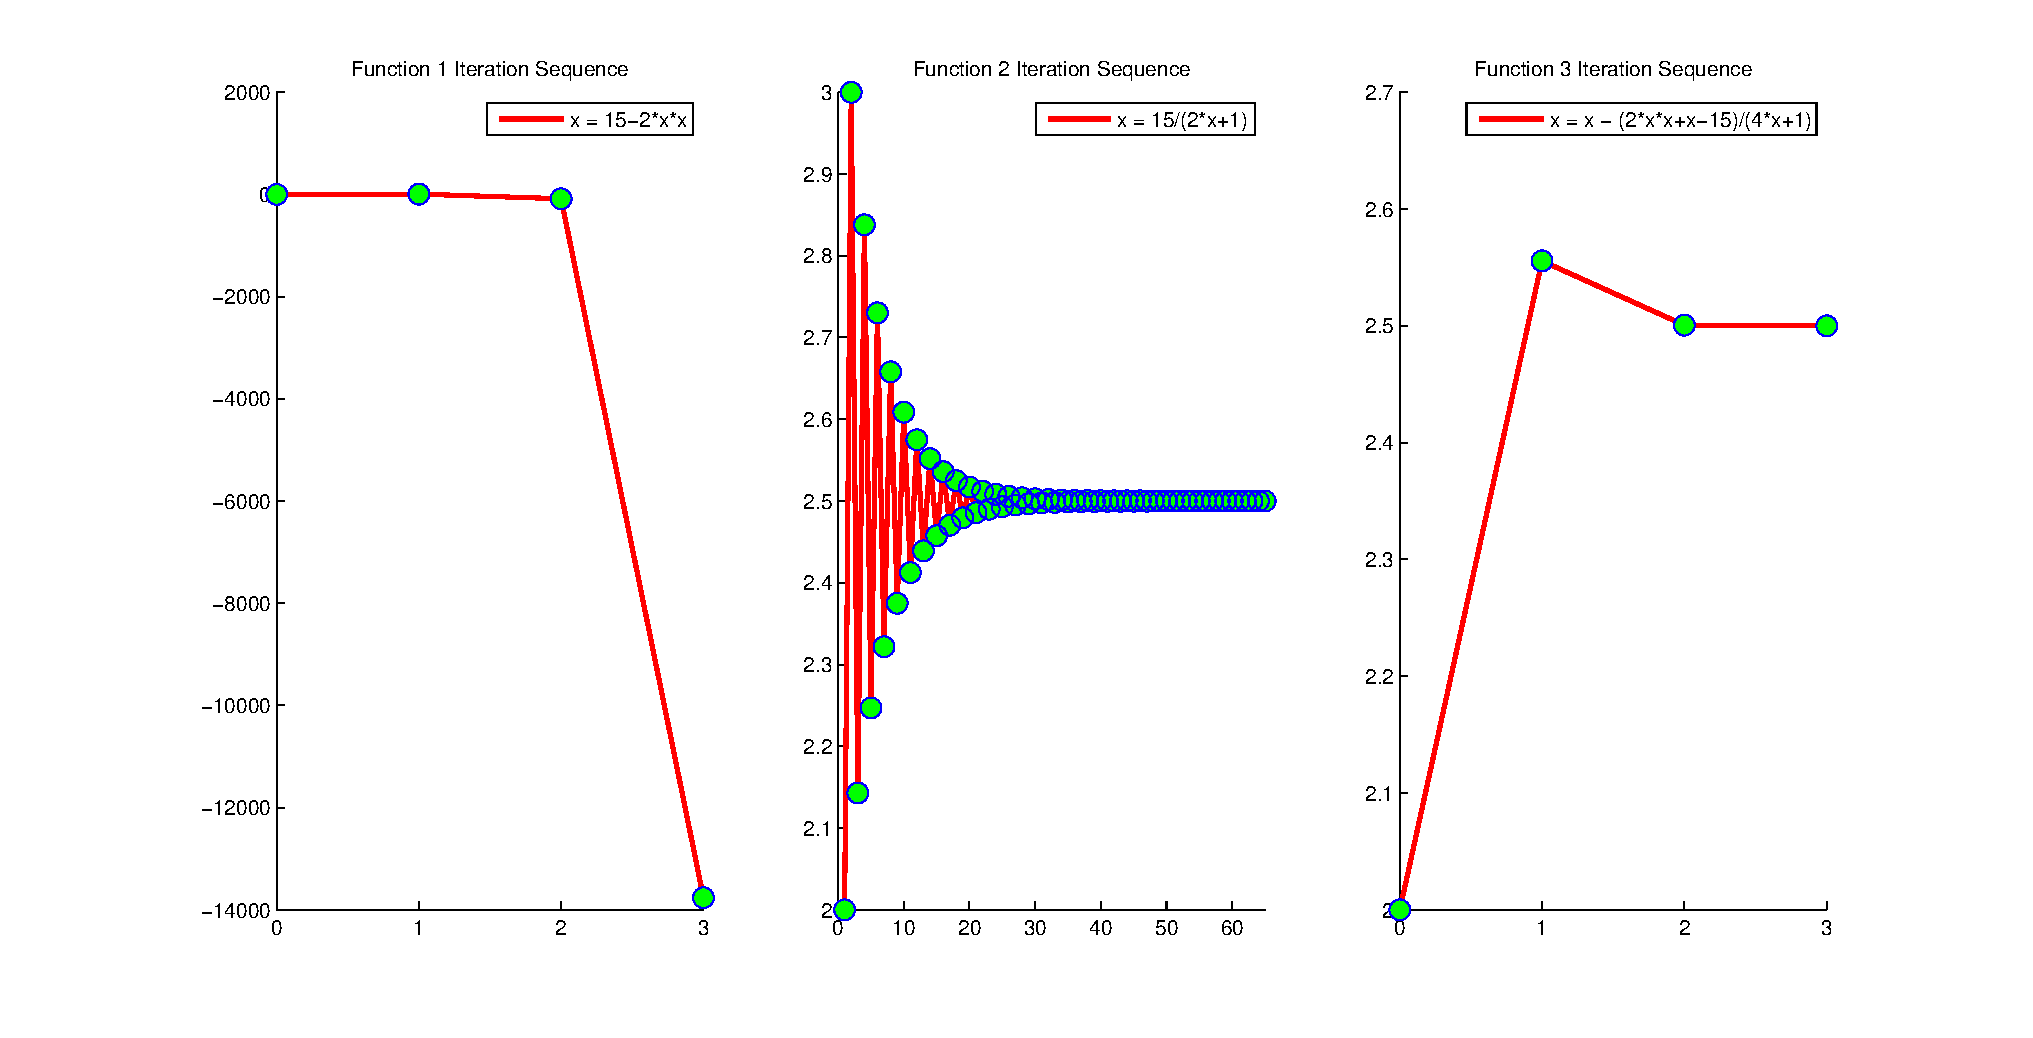
\includegraphics[width=1.0\textwidth]{../chapter2_1_0.eps}
						\caption{不动点法迭代序列. 左图为$x_{k+1} = 15 - x_k^2$迭代序列, 在第$3$次迭代后, 取值已经过大. 此后迭代序列将很快溢出. 中图为$x_{k+1} = \frac{15}{2x_k+1}$, 右图为$x_{k+1} = x_k - \frac{2x_k^2+x_k-15}{4x_k+1}$. 可以观察出, $x_{k+1} = x_k - \frac{2x_k^2+x_k-15}{4x_k+1}$收敛速率更快}
						\label{img_chapter2_1_0}
					\end{figure}
				\begin{center}
					\begin{tabular}{|c|c|c|c|c|}
						\hline
						迭代函数 & 迭代次数 & 解 & 迭代停止条件 & 初始值 \\
						\hline
						$x_{k+1} = 15 - x_k^2$ & - & No Solution &$\left|f\left(x\right) - x\right| < TOL$ & $x_0=2$ \\
						\hline
						$x_{k+1} = \frac{15}{2x_k+1}$&  64 & 2.499995 & $\left|f\left(x\right) - x\right| < TOL$&$x_0 = 2$ \\
						\hline
						$x_{k+1} = x_k - \frac{2x_k^2+x_k-15}{4x_k+1}$ & 3 & 2.500000 & $\left|f\left(x\right) - x\right| < TOL$ & $x_0=2$ \\
						\hline
					\end{tabular}	
				\end{center}
			\paragraph{稳定性测试}:
				略微改变初值$x_0$, 观察解是否发生变化. 取$x_0^{*} = x_0 \pm 0.05,0.10,0.20$.
			
				\begin{figure}[H]
					\centering
					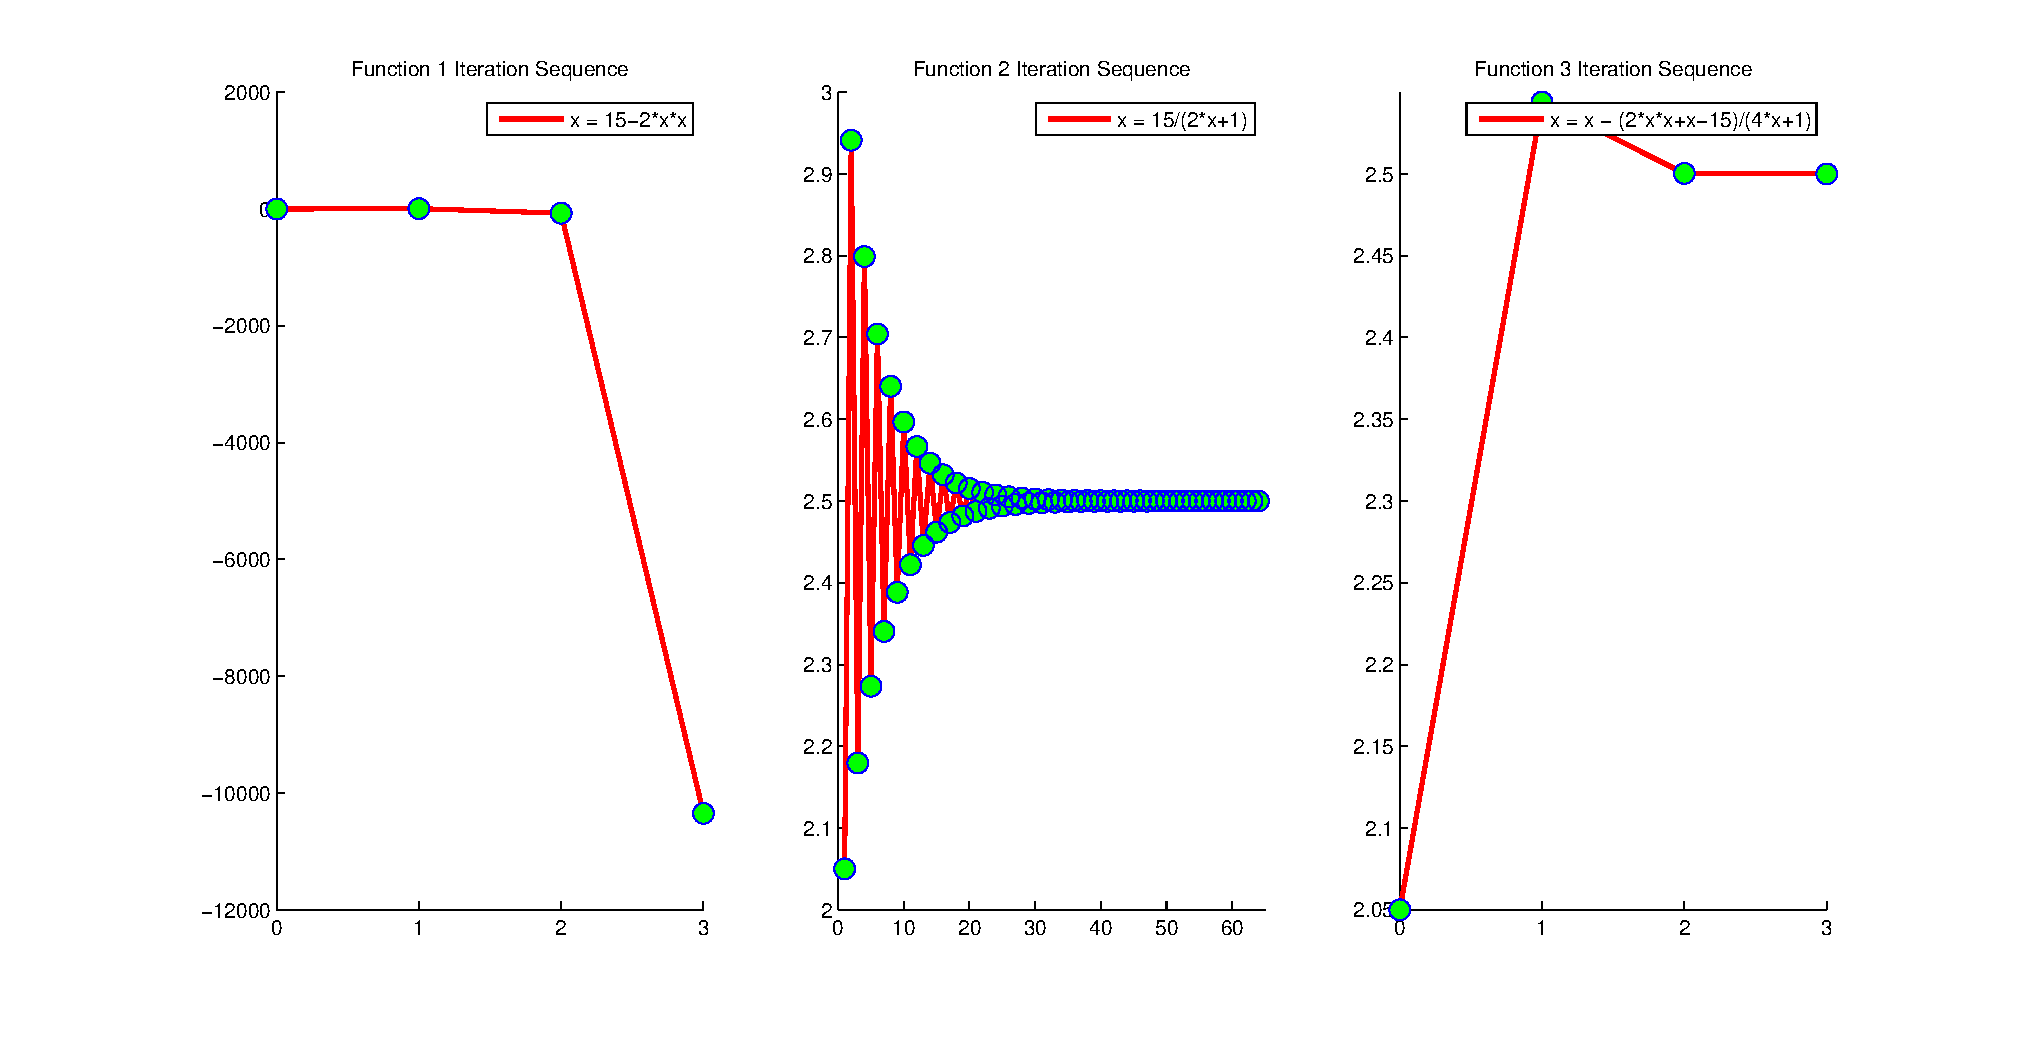
\includegraphics[width=1.0\textwidth]{../chapter2_1_0_1.eps}
					\caption{不动点法迭代序列, $x_0^{*} = x_0 + 0.05$. 收敛性与初值$x_0$时相同.}
					\label{img_chapter2_1_0_1}
				\end{figure}
			
				\begin{figure}[H]
					\centering
					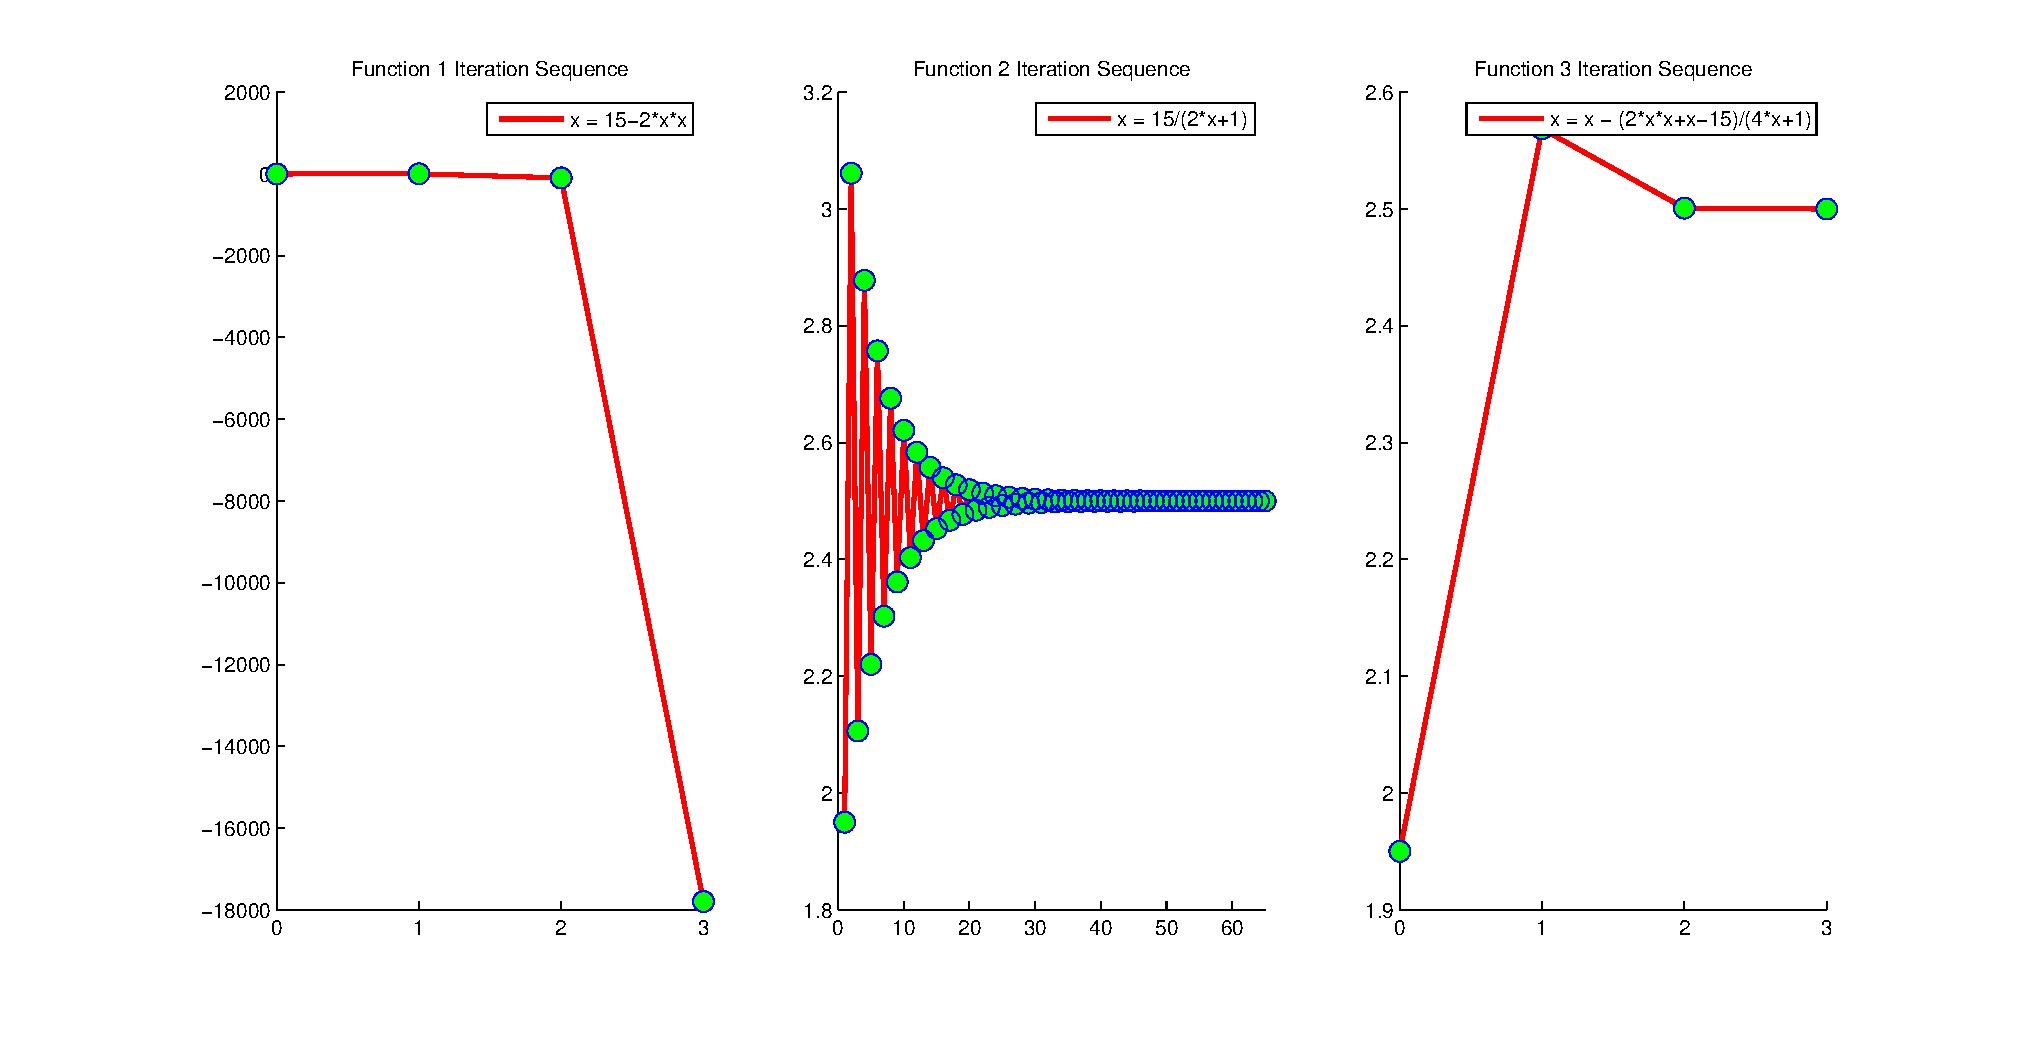
\includegraphics[width=1.0\textwidth]{../chapter2_1_0_2.eps}
					\caption{不动点法迭代序列, $x_0^{*} = x_0 - 0.05$. 收敛性与初值$x_0$时相同.}
					\label{img_chapter2_1_0_2}
				\end{figure}
				
				\begin{figure}[H]
					\centering
					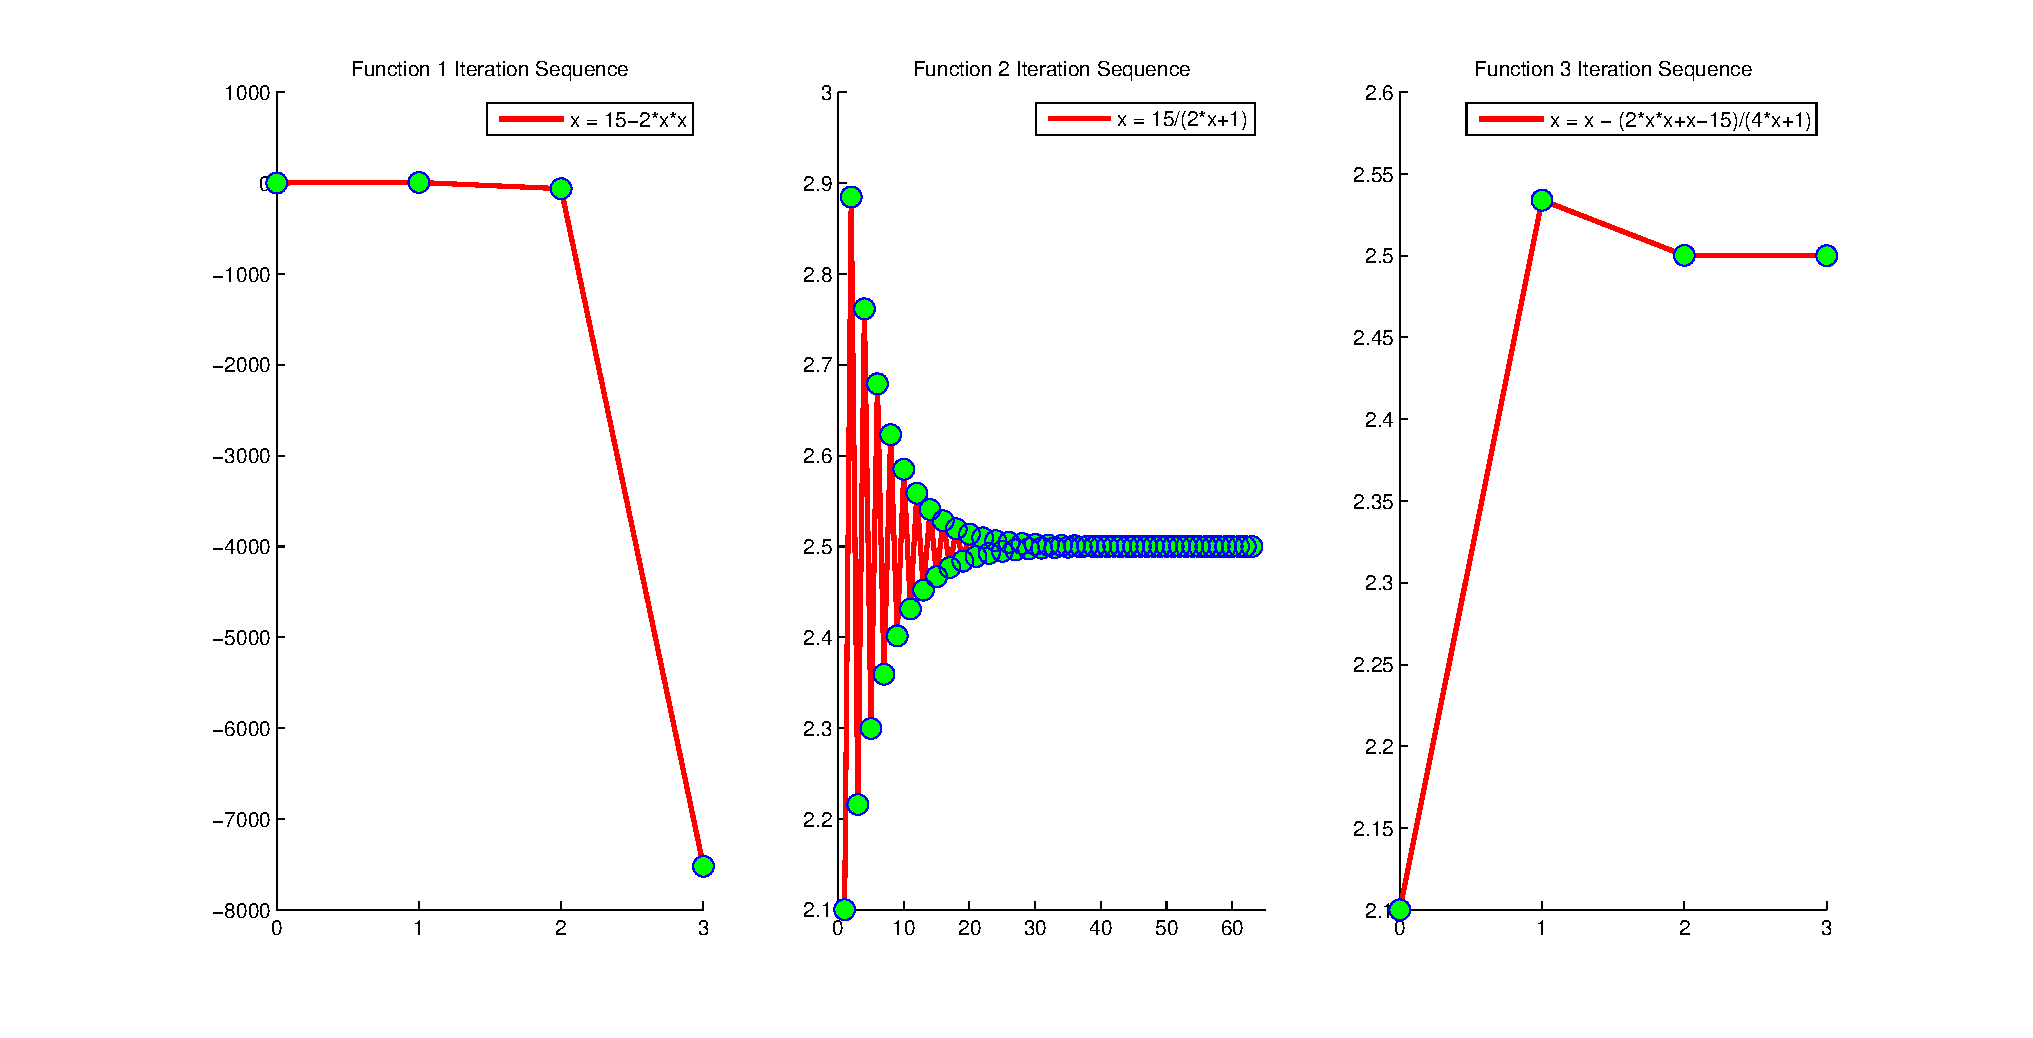
\includegraphics[width=1.0\textwidth]{../chapter2_1_0_3.eps}
					\caption{不动点法迭代序列, $x_0^{*} = x_0 + 0.10$. 收敛性与初值$x_0$时相同.}
					\label{img_chapter2_1_0_3}
				\end{figure}
				
				\begin{figure}[H]
					\centering
					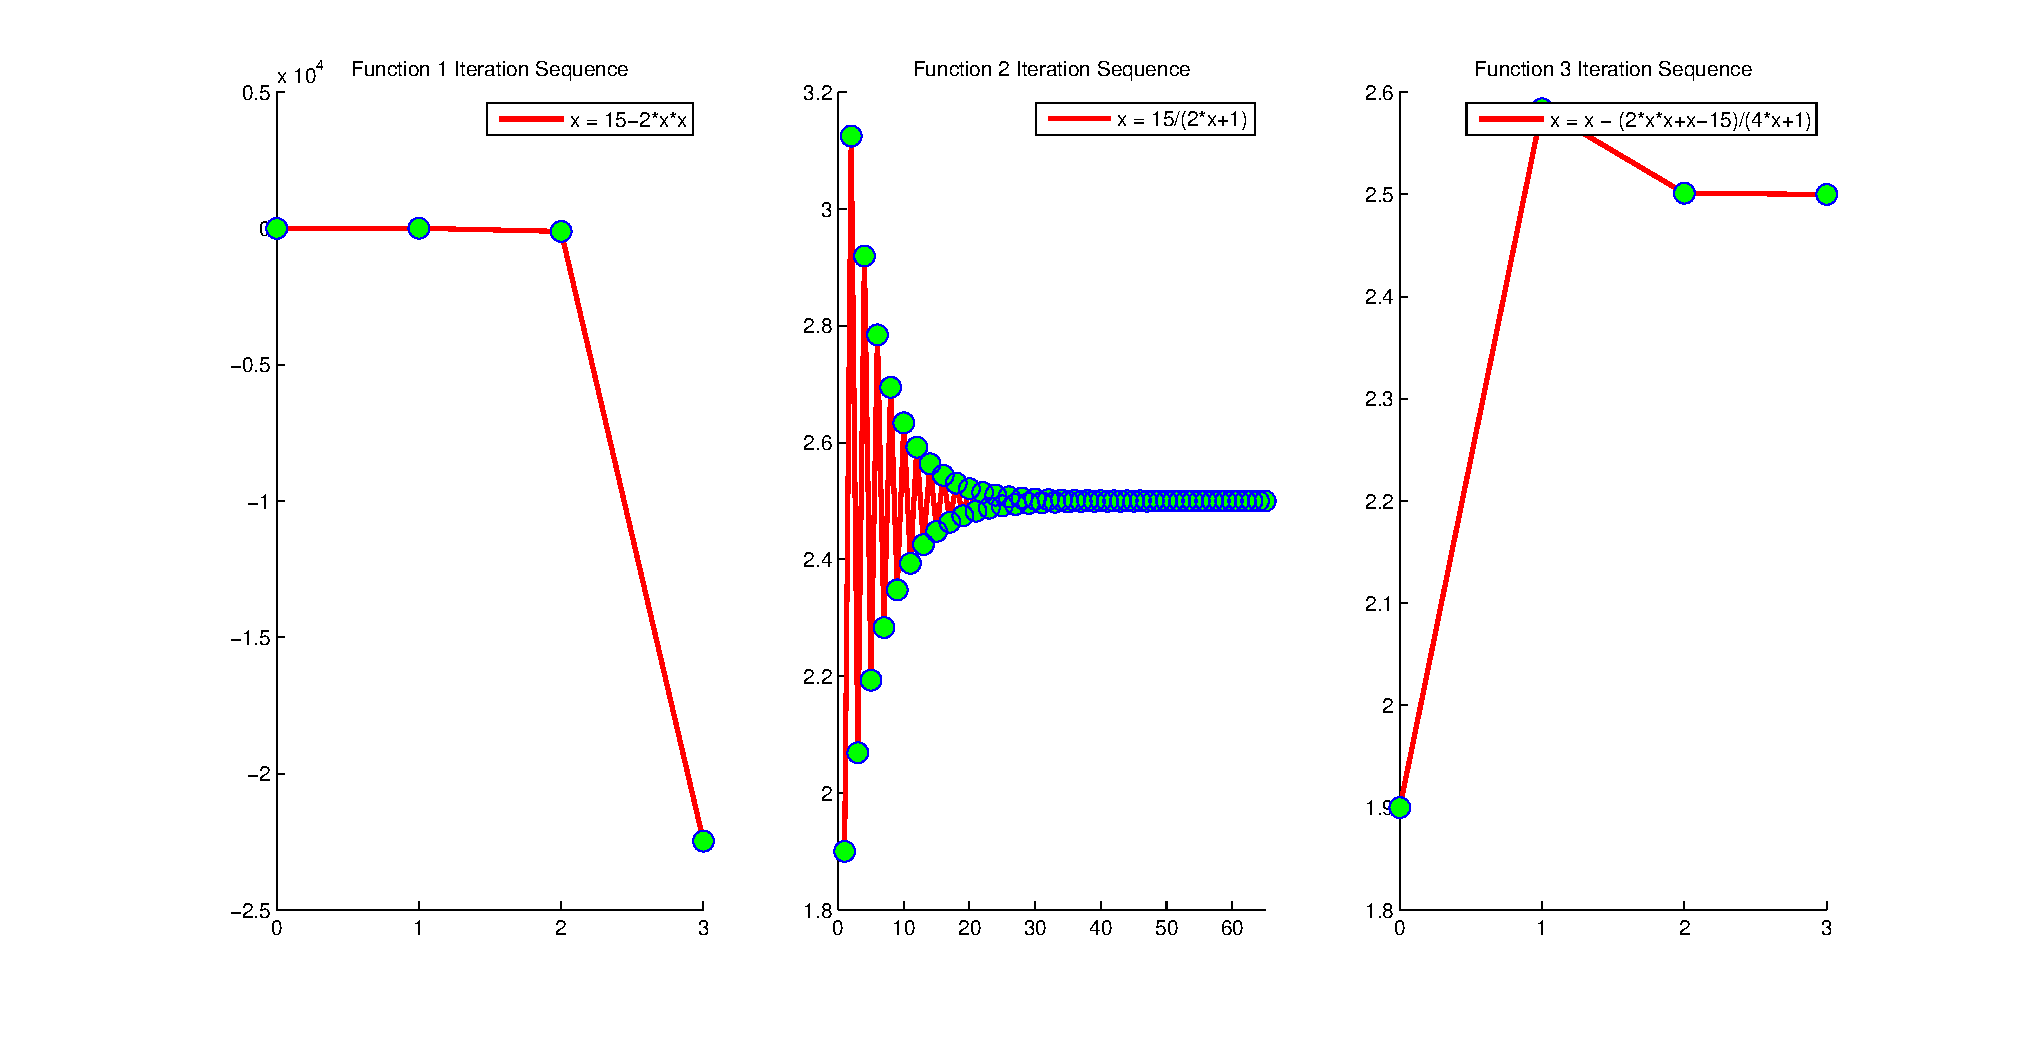
\includegraphics[width=1.0\textwidth]{../chapter2_1_0_4.eps}
					\caption{不动点法迭代序列, $x_0^{*} = x_0 - 0.10$. 收敛性与初值$x_0$时相同.}
					\label{img_chapter2_1_0_4}
				\end{figure}
				
				稳定性测试结果:\\
				\begin{center}
					\begin{tabular}{|c|c|c|c|c|c|c|}
						\hline
						&\multicolumn{2}{|c|}{$x = f_1\left(x\right)$}  & \multicolumn{2}{|c|}{$x = f_2\left(x\right)$} &\multicolumn{2}{|c|}{$x = f_3\left(x\right)$} \\
						\hline
						$x_0^{*} = x_0 + 0.05$ & \multicolumn{2}{|c|}{No Solution} & 63& 2.500005& 3&2.500000 \\
						\hline
						$x_0^{*} = x_0 - 0.05$ & \multicolumn{2}{|c|}{No Solution} &64 &2.499995 & 3& 2.500000\\
						\hline
						$x_0^{*} = x_0 + 0.10$ & \multicolumn{2}{|c|}{No Solution} & 62&2.499995 &3 &2.500000 \\
						\hline
						$x_0^{*} = x_0 - 0.10$ & \multicolumn{2}{|c|}{No Solution} & 65& 2.500005& 3&2.500000 \\
						\hline
						$x_0^{*} = x_0 + 0.20$ & \multicolumn{2}{|c|}{No Solution} &61 &2.500005 & 3& 2.500000\\
						\hline
						$x_0^{*} = x_0 - 0.20$ & \multicolumn{2}{|c|}{No Solution} & 66&2.499995 &3 &2.500001 \\
						\hline
					\end{tabular}
				\end{center}
			
				\begin{figure}[H]
					\centering
					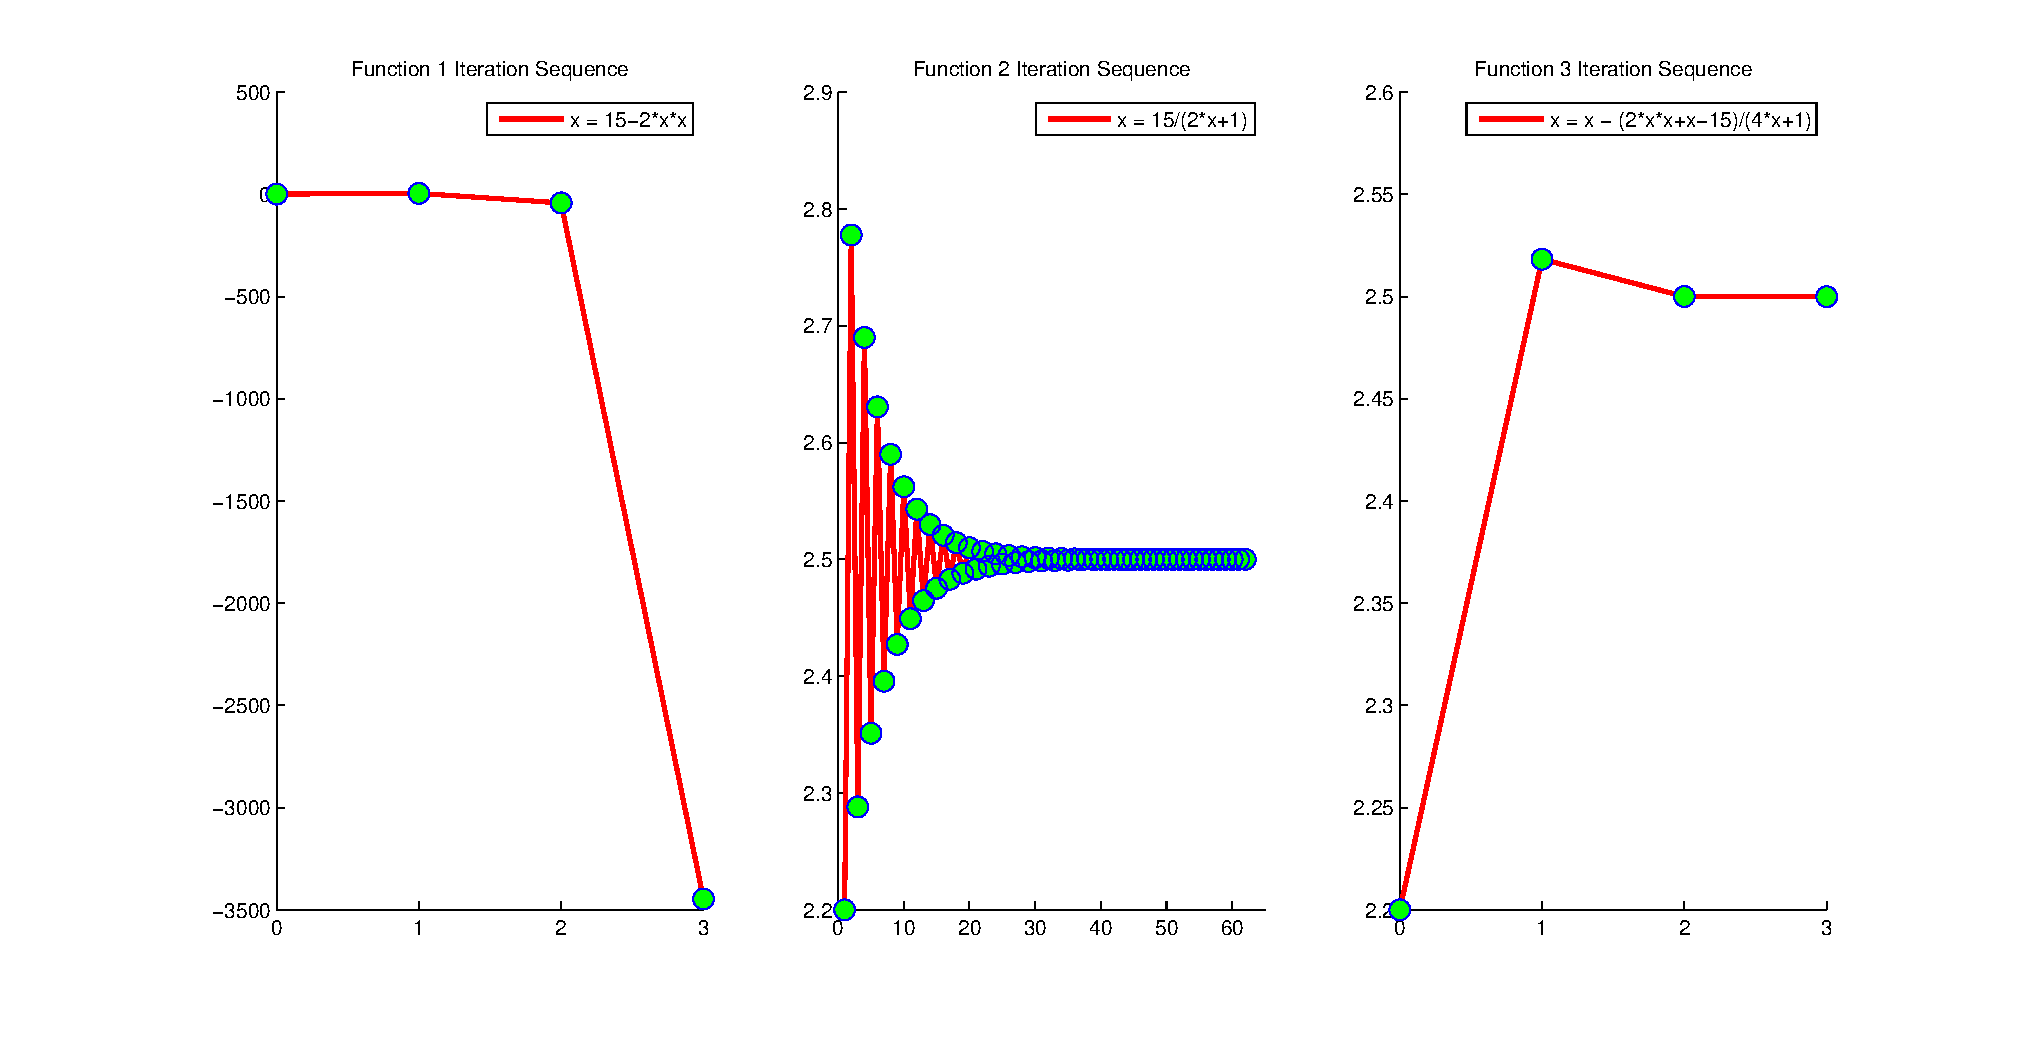
\includegraphics[width=1.0\textwidth]{../chapter2_1_0_5.eps}
					\caption{不动点法迭代序列, $x_0^{*} = x_0 + 0.20$. 收敛性与初值$x_0$时相同.}
					\label{img_chapter2_1_0_5}
				\end{figure}
				
				\begin{figure}[H]
					\centering
					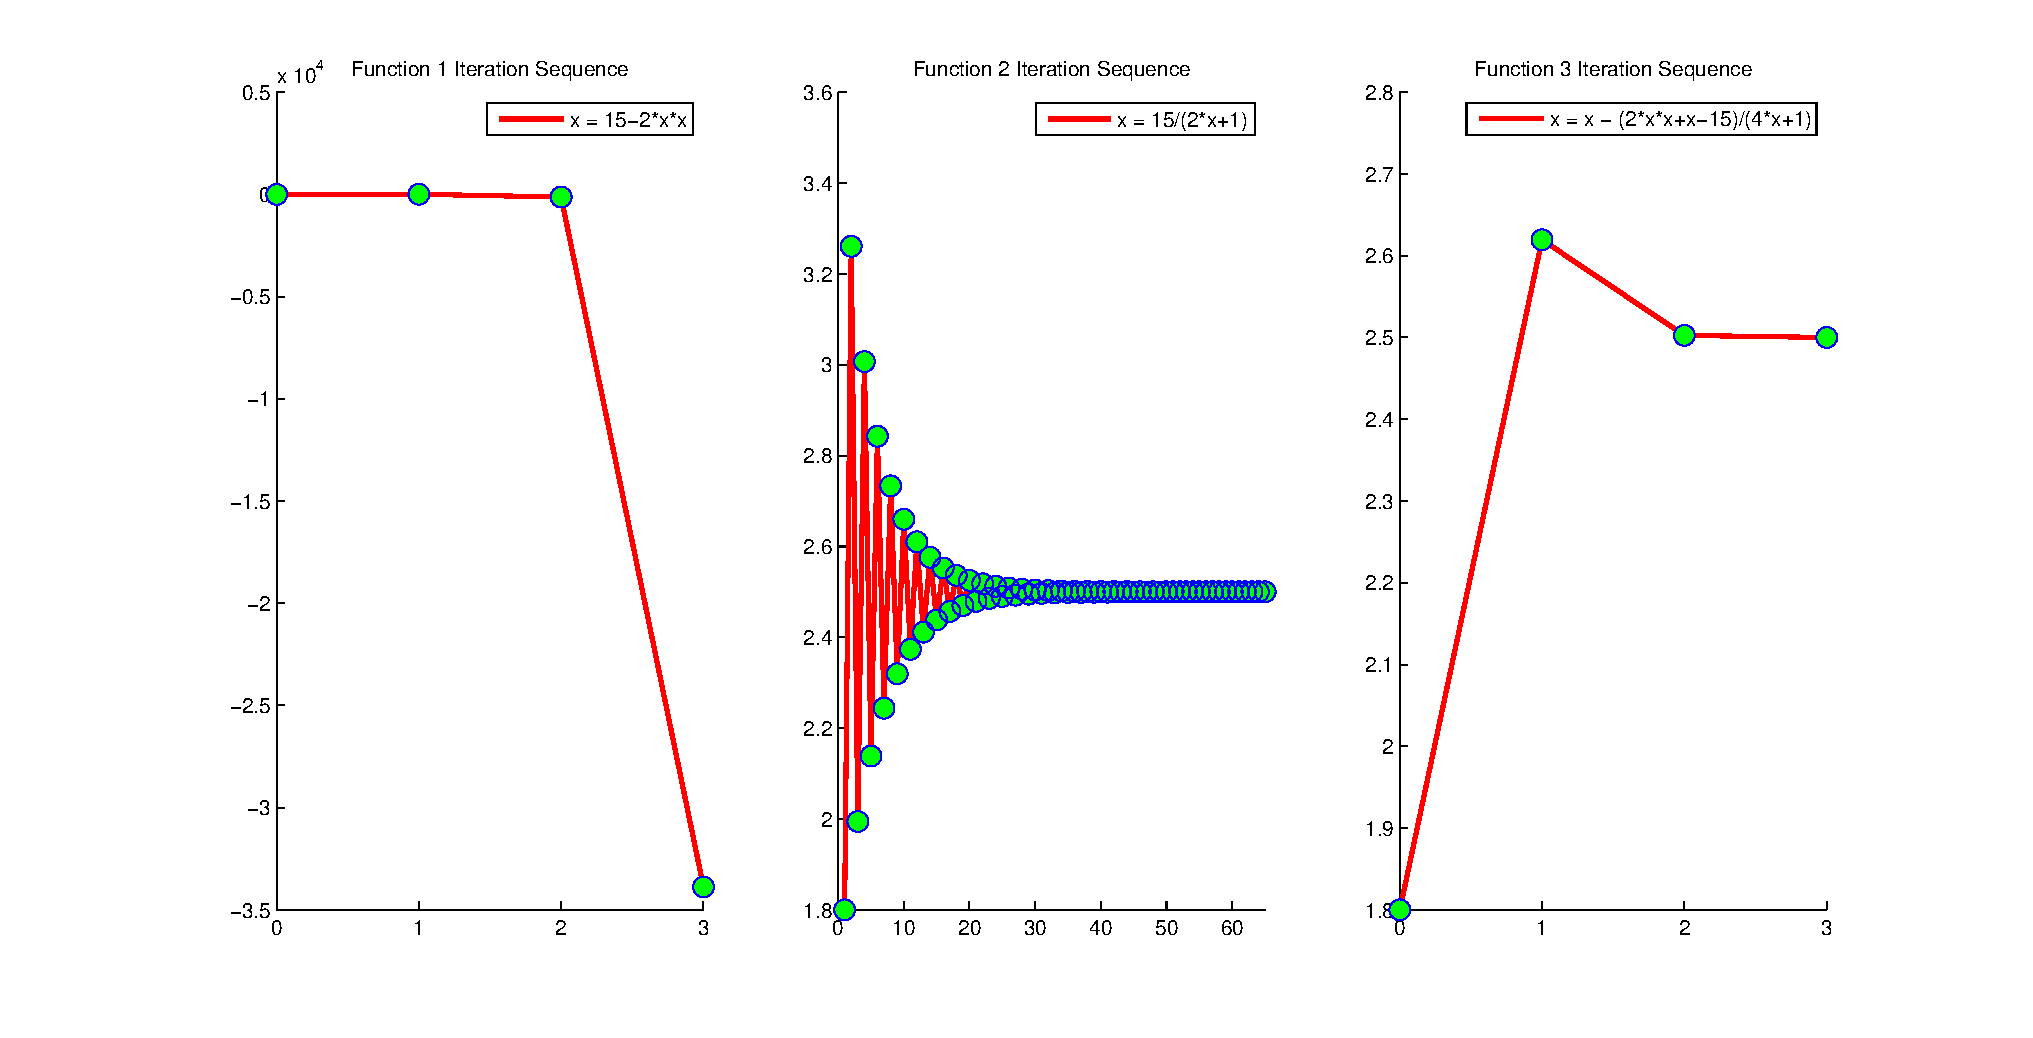
\includegraphics[width=1.0\textwidth]{../chapter2_1_0_6.eps}
					\caption{不动点法迭代序列, $x_0^{*} = x_0 - 0.20$. 收敛性与初值$x_0$时相同.}
					\label{img_chapter2_1_0_6}
				\end{figure}
			
			\paragraph{Analysis}:\newline
				\begin{enumerate}
					\item 对于迭代$x^k=f_1\left(x_{k-1}\right)$, 当$x \in \left[0,4\right]$时, $-17 \leq f_1\left(x\right) \leq 15 $. 对于给定的初始点所在邻域, 不满足不动点迭代条件$f_1\left(x\right) \in \left[0,4\right]$, 即该迭代发散.
					\item 对于迭代$x^k=f_2\left(x_{k-1}\right)$, 当$x \in \left[1.5,4.5\right]$时, $f_2\left(x\right) \in \left[1.5,4.5\right]$, 满足不动点迭代条件, 该迭代收敛.
					\item 对于迭代$x^k=f_3\left(x_{k-1}\right)$, 当$x \in \left[1.5,4.5\right]$时, $f_3\left(x\right) \in \left[1.5,4.5\right]$, 满足不动点迭代条件, 该迭代收敛. 在此区间上, 由于$\max \left|f_3^{'} \left(x \right)   \right| <\max 
					\left|f_2^{'}\left(x\right) \right|$, 因此使用$x^k=f_3\left(x_{k-1}\right)$收敛速率更快速.
				\end{enumerate}
		\subsection{Problem 2}
			\paragraph{题目描述}
			:\newline
				证明方程$2-3x-\sin\left(x\right) = 0$在$\left(0,1\right)$内有且仅有一个实根, 使用二分法求误差不大于$0.0005$的根, 以及需要的迭代次数.
			\paragraph{Proof}
			:\newline
				令$f\left(x\right) = 2 - 3x - \sin\left(x\right)$.\\
				则$f'\left(x\right) = -3 - \cos \left(x\right) < 0$.\\
				而$f\left(0\right) = 2 > 0, f\left(1\right) = 1 - \sin\left(1\right) < 0$\\
				因此方程$2-3x-\sin\left(x\right) = 0$在$\left(0,1\right)$内有且仅有一个实根.
				
			\begin{lstlisting}[language=Matlab]
				f = @(x)2-3*x-sin(x);
				TOL = 0.0005; N = 100; Left = 0.0; Right = 1.0;
				X = Left:(Right-Left)/400:Right;
				Y = 2 - 3*X - sin(X);
				FL = f(Left); CNT = 0; Mid = 0; A = [];
				while CNT < N
					CNT = CNT + 1;
					Mid = (Left + Right)/2; FMid = f(Mid); A(CNT) = FMid;
					if FL*FMid < 0
						Right = Mid;
					else
						if FL*FMid == 0
							break
						else
							FL = FMid; Left = Mid;
						end
					end
					if Right - Left < TOL
						break
					end
				end
				subplot(1,2,1);
				plot(X,Y,Mid,FMid,'o',[Mid,Mid],[min(Y),max(Y)],'r:',[X(1),X(length(X))],[FMid,FMid],':r');
				title('Zero Point of Function')
				legend('2-3*x-sin(x)','Zero Point')
				subplot(1,2,2);
				plot(1:CNT,A,'o',1:CNT,A,'-r');
				title('Iteration Sequence of f(x)');
				legend('f(x) of each iteration')
				fprintf('Total time of iteration is %d. The answer is %f.',CNT,Mid)
			\end{lstlisting}
			
			\paragraph{输出}
			:\newline
				Total time of iteration is $11$. The answer is $0.505371$.
				\subparagraph{Iteration Sequence Graph}
				\begin{figure}[H]
					\centering
					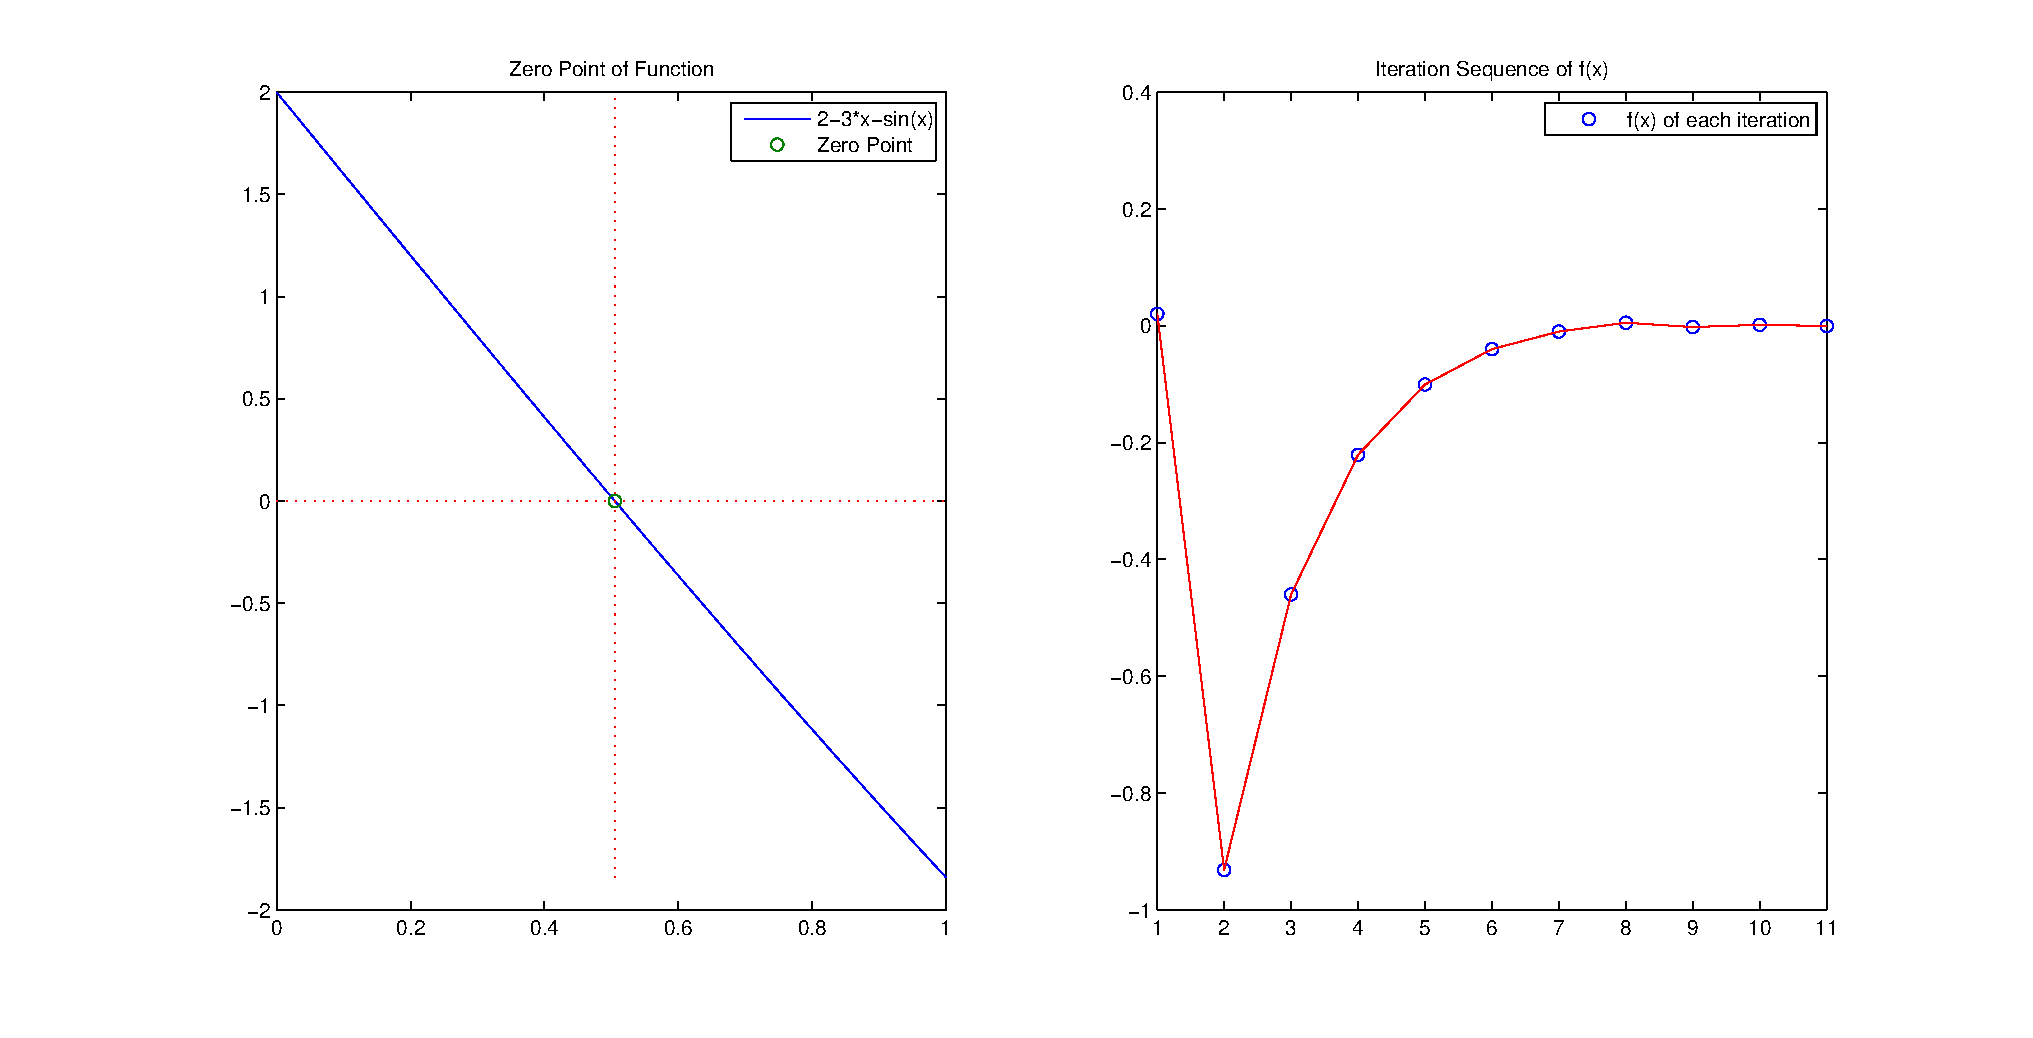
\includegraphics[width=1.0\textwidth]{../chapter_2_1_1.eps}
					\caption{二分法迭代结果. 左图为计算出的零点, 右图为$f\left(x\right)$迭代序列}
					\label{img_chapter2_1_1}
				\end{figure}
			\paragraph{二分法误差分析}
			:\newline	
		\subsection{Problem 3}
			\paragraph{题目描述}
			:\newline
				利用牛顿法求解方程\newline
				$\frac{1}{2} + \frac{1}{4}x^2 - x\sin\left(x\right) - \frac{1}{2}\cos\left(2x\right) = 0$
				分别取$x_0 = \frac{\pi}{2},5\pi,10\pi$, 使得精度不超过$10^{-5}$, 比较初值对计算结果的影响.
			\paragraph{牛顿法推导}:\newline
				假设$f\in C^2\left[a,b\right]$, 并且$x^{*}$是$f\left(x \right) = 0$的一个解.
			
				令$\overline{x} \in \left[a,b\right]$是对$x_{*}$的一个近似, 使得$f'\left(\overline{x} \right) \neq 0$且$\left|\overline{x} - x^{*} \right|$比较小.
			
				考虑$f\left(x\right)$在$\overline{x}$处展开的一阶泰勒多项式$f\left(x\right) = f\left(\overline{x} \right) + \left(x - \overline{x}\right) f' \left(\overline{x} \right) + \frac{\left(x-\overline{x}\right)^2}{2}f^{''}\left(\xi \left(x\right) \right)$, 其中$\xi \left(x \right)$在$x$和$\overline{x}$之间.
			
				因为$f\left(x^{*}\right)=0$, 令$x=x^{*}$, 此时有
				$0 = f\left(x^{*}\right) = f\left(\overline{x} \right) + \left(x^{*} - \overline{x}\right) f' \left(\overline{x} \right) + \frac{\left(x^{*}-\overline{x}\right)^2}{2}f^{''}\left(\xi \left(x\right) \right)$.
			
				忽略余项, 得到
				$0 = f\left(x^{*}\right) \approx f\left(\overline{x} \right) + \left(x^{*} - \overline{x}\right) f' \left(\overline{x} \right)$
			
				求得$x^{*} \approx \overline{x} - \frac{f\left(\overline{x}\right)}{f'\left(\overline{x}\right)}$
			
				因此定义迭代序列为:
				$x_n = x_{n-1} - \frac{f\left(x_{n-1} \right)}{f'\left(x_{n-1} \right)},\forall n \geq 1$.
				
			\paragraph{Code}:\newline
				\begin{lstlisting}
				clear;clc;
				f = @(x)0.5+0.25*x^2-x*sin(x)-0.5*cos(2*x);
				x0 = pi*5;
				diff_f = @(x)x/2 + sin(2*x) - sin(x) - x*cos(x);              
				TOL = 5e-5; N = 1000; CNT = 1; A = x0;
				while CNT < N
					CNT = CNT + 1;
					x = x0 - f(x0)/diff_f(x0); A(CNT) = x;
					if abs(x - x0) < TOL
						fprintf('Total time of iteration is %d. The answer is %f.',CNT,A(CNT))
						return;
					end
					x0 = x;
				end
				disp('No Solution');
				\end{lstlisting}
			
			\paragraph{Analysis}:\newline
			\begin{figure}[H]
				\centering
				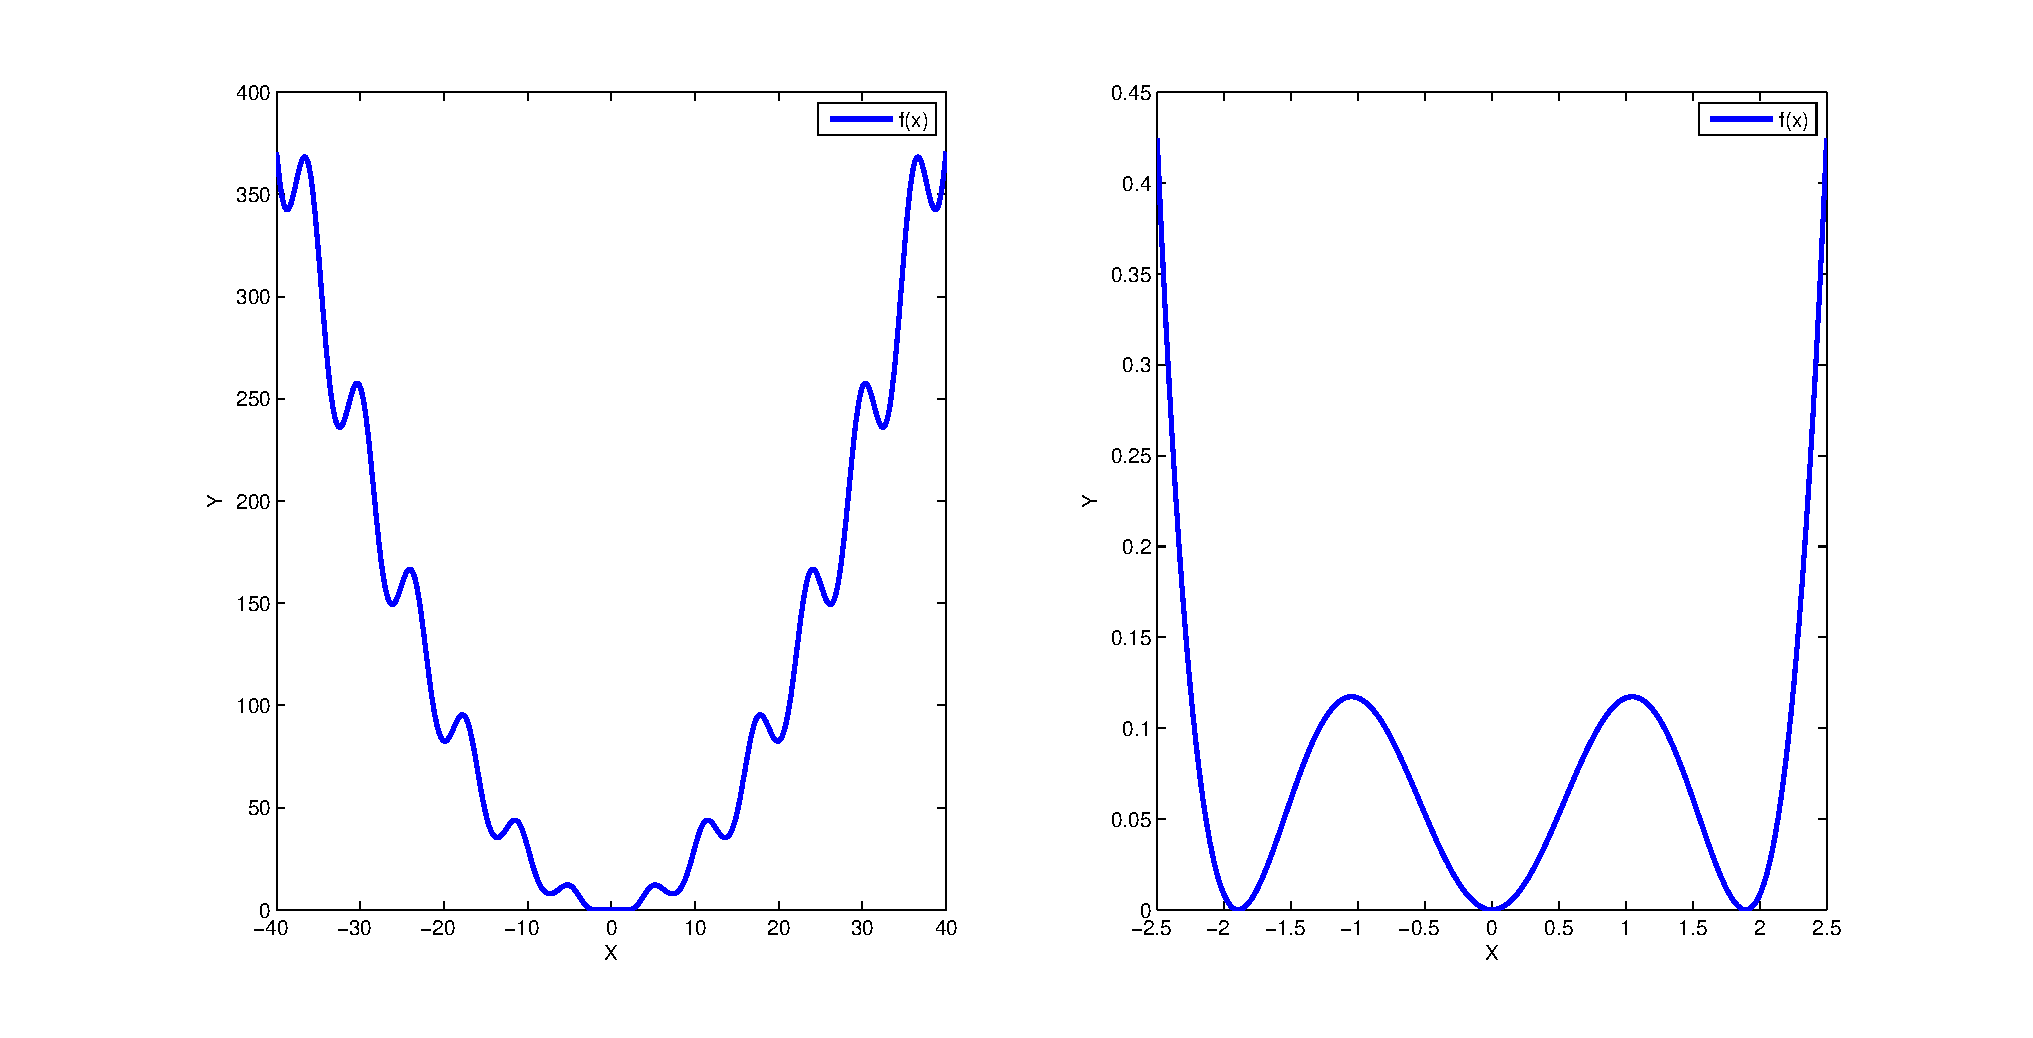
\includegraphics[width=1.0\textwidth]{../chapter2_3_1.eps}
				\caption{函数图像. 观察左图可以发现, $\lim\limits_{x \to \infty}f\left(x\right) = + \infty$, 函数的零点在$x=0$附近. 观察右图可以发现, $f\left(x\right)$的一个零点位于$x=0$处, 一个零点位于$\left(1.5,2\right)$, 一个零点位于$\left(-2,-1.5\right)$. 根据初始值不同, 牛顿法迭代可能收敛到不同的零点, 也可能不收敛.}
				\label{img_chapter2_3_1}
			\end{figure}
			\paragraph{Answer}
				\begin{center}
					\begin{tabular}{|c|c|c|c|}
						\hline
						初始值$x_0$ & $\pi /2$ & $5\pi$ & $10\pi$ \\
						\hline
						迭代次数 & 12 &16 & 不收敛\\
						\hline
						零点 & 1.895447& 1.895452& -\\
						\hline
						TOL &5e-5 &5e-5 &5e-5 \\
						\hline
					\end{tabular}
				\end{center}
				\begin{figure}[H]
					\centering
					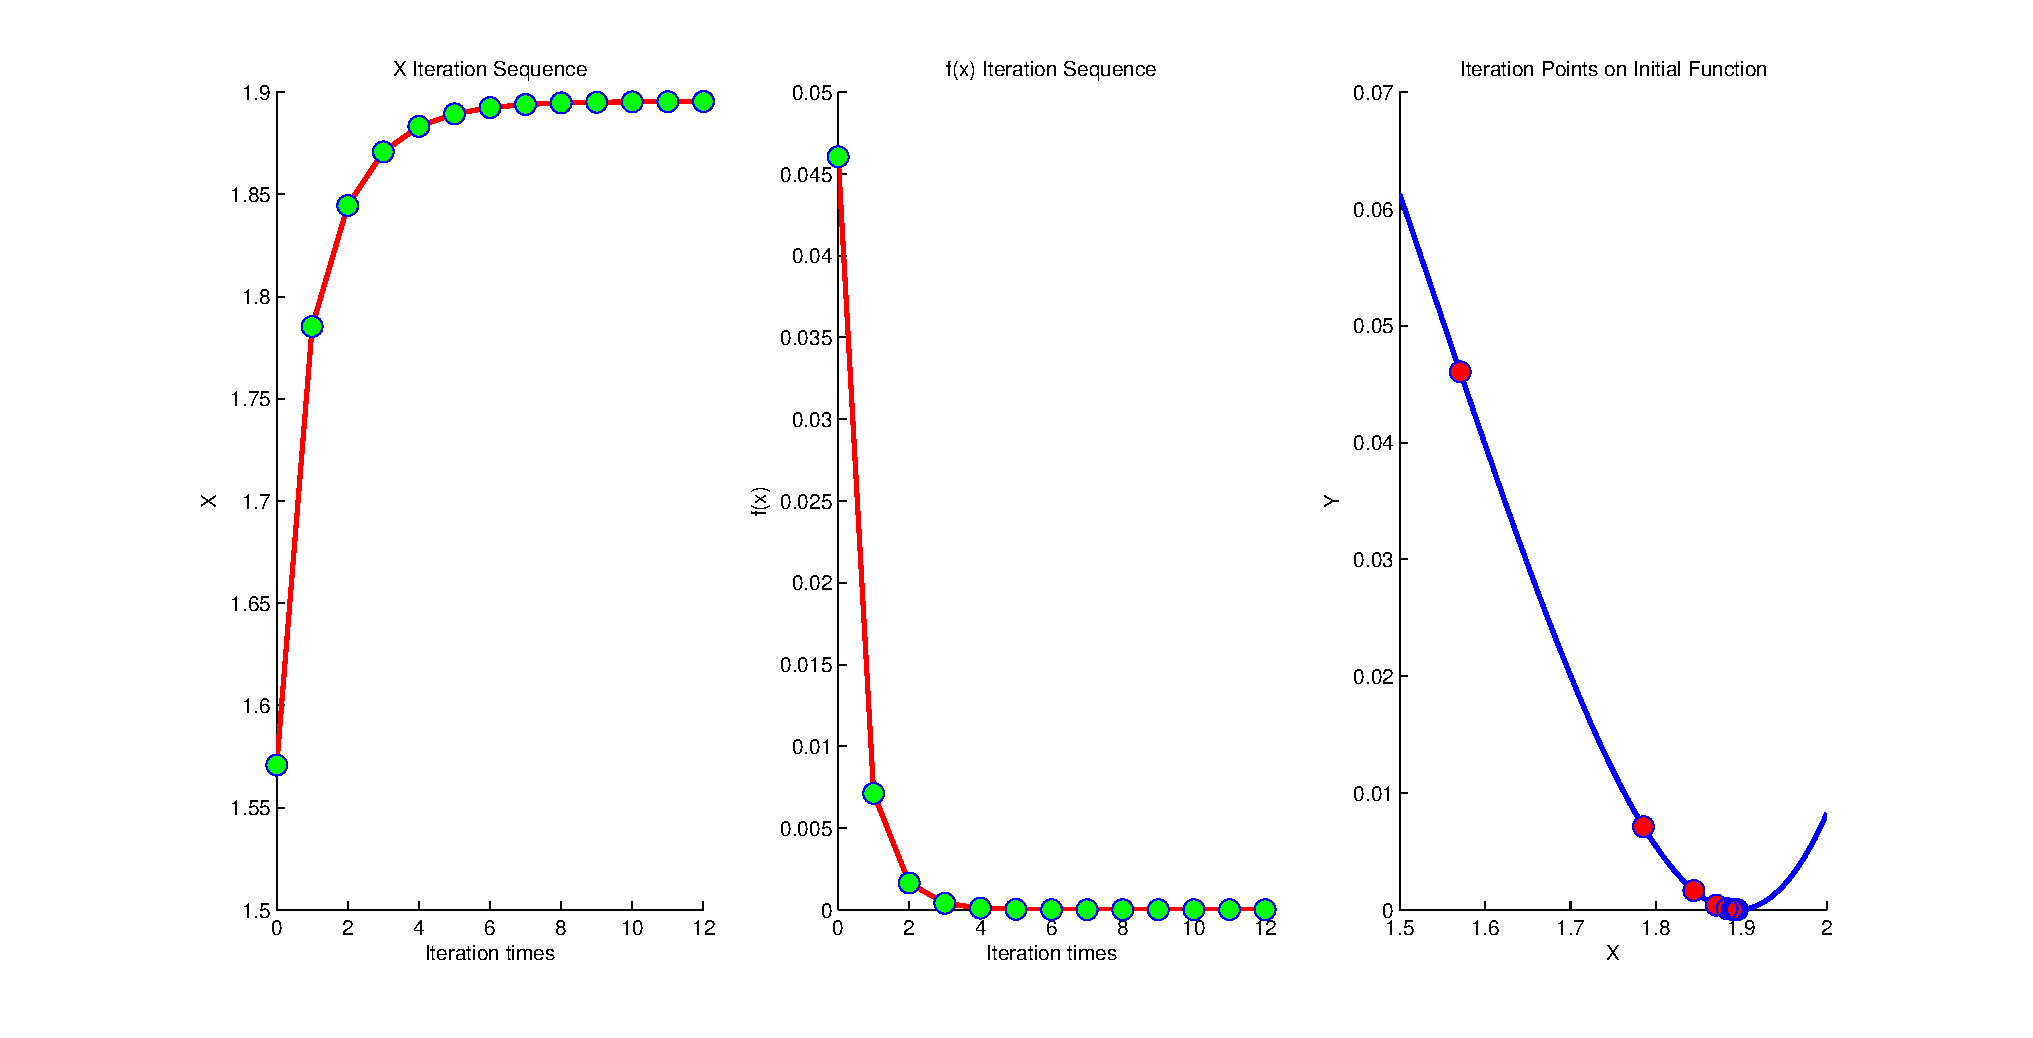
\includegraphics[width=1.0\textwidth]{../chapter2_3_2.eps}
					\caption{$x_0 = \pi /2$. 左图: $x$迭代序列. 中图: 迭代序列对应的$f\left(x\right)$值. 右图: 迭代点在函数图像上的分布}
					\label{img_chapter2_3_2}
				\end{figure}
				\begin{figure}[H]
					\centering
					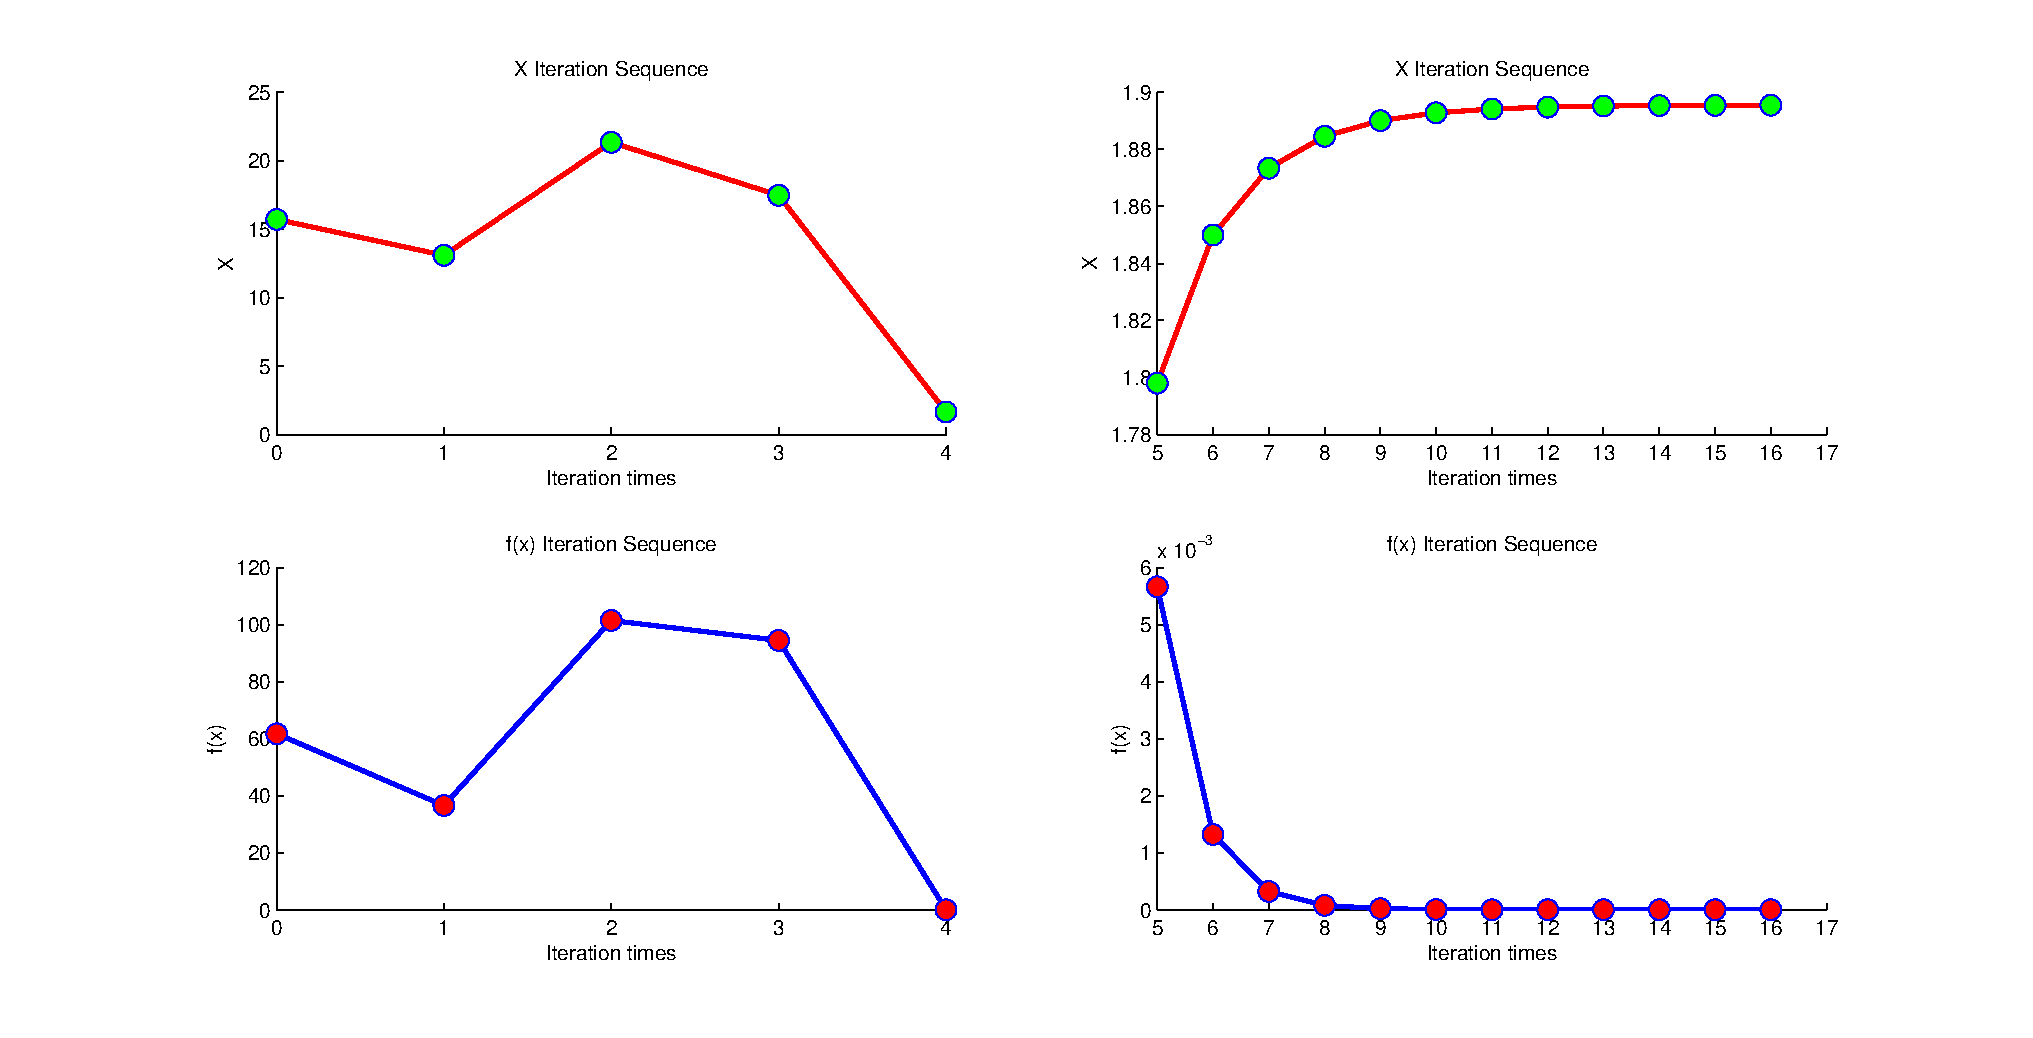
\includegraphics[width=1.0\textwidth]{../chapter2_3_3.eps}
					\caption{$x_0 = 5\pi$. 左上: $x$迭代序列($t = 0,1,2,3,4$); 右上: $x$迭代序列($t = 5,\cdots,16$); 左下: 迭代序列对应的$f\left(x\right)$值($t = 0,1,2,3,4$); 右下: 迭代序列对应的$f\left(x\right)$值($t = 5.\cdots,16$)}
					\label{img_chapter2_3_3}
				\end{figure}
				\begin{figure}[H]
					\centering
					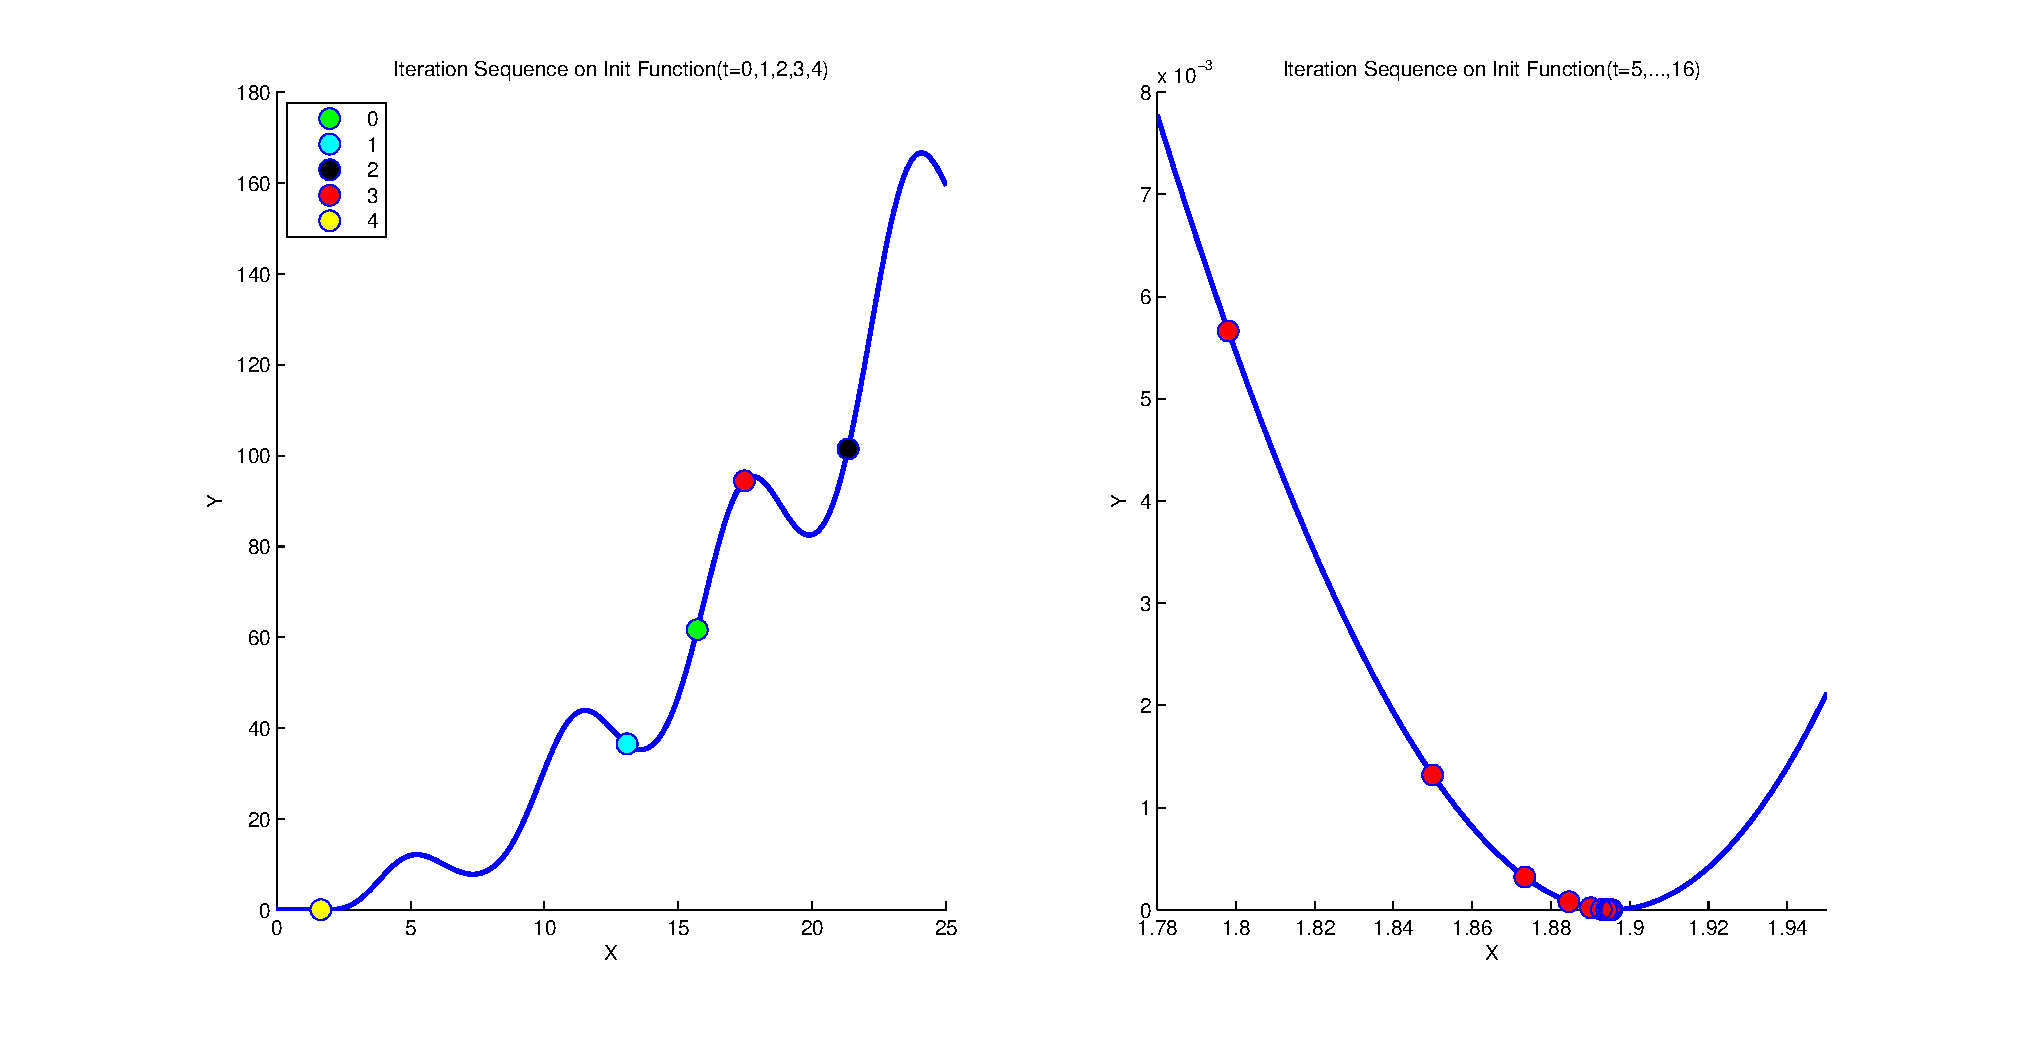
\includegraphics[width=1.0\textwidth]{../chapter2_3_4.eps}
					\caption{$x_0 = 5\pi$. 左图: 迭代点在函数图像上的分布($t = 0,1,2,3,4$); 右上:迭代点在函数图像上的分布($t = 0,1,2,3,4$)}
					\label{img_chapter2_3_4}
				\end{figure}
				\begin{figure}[H]
					\centering
					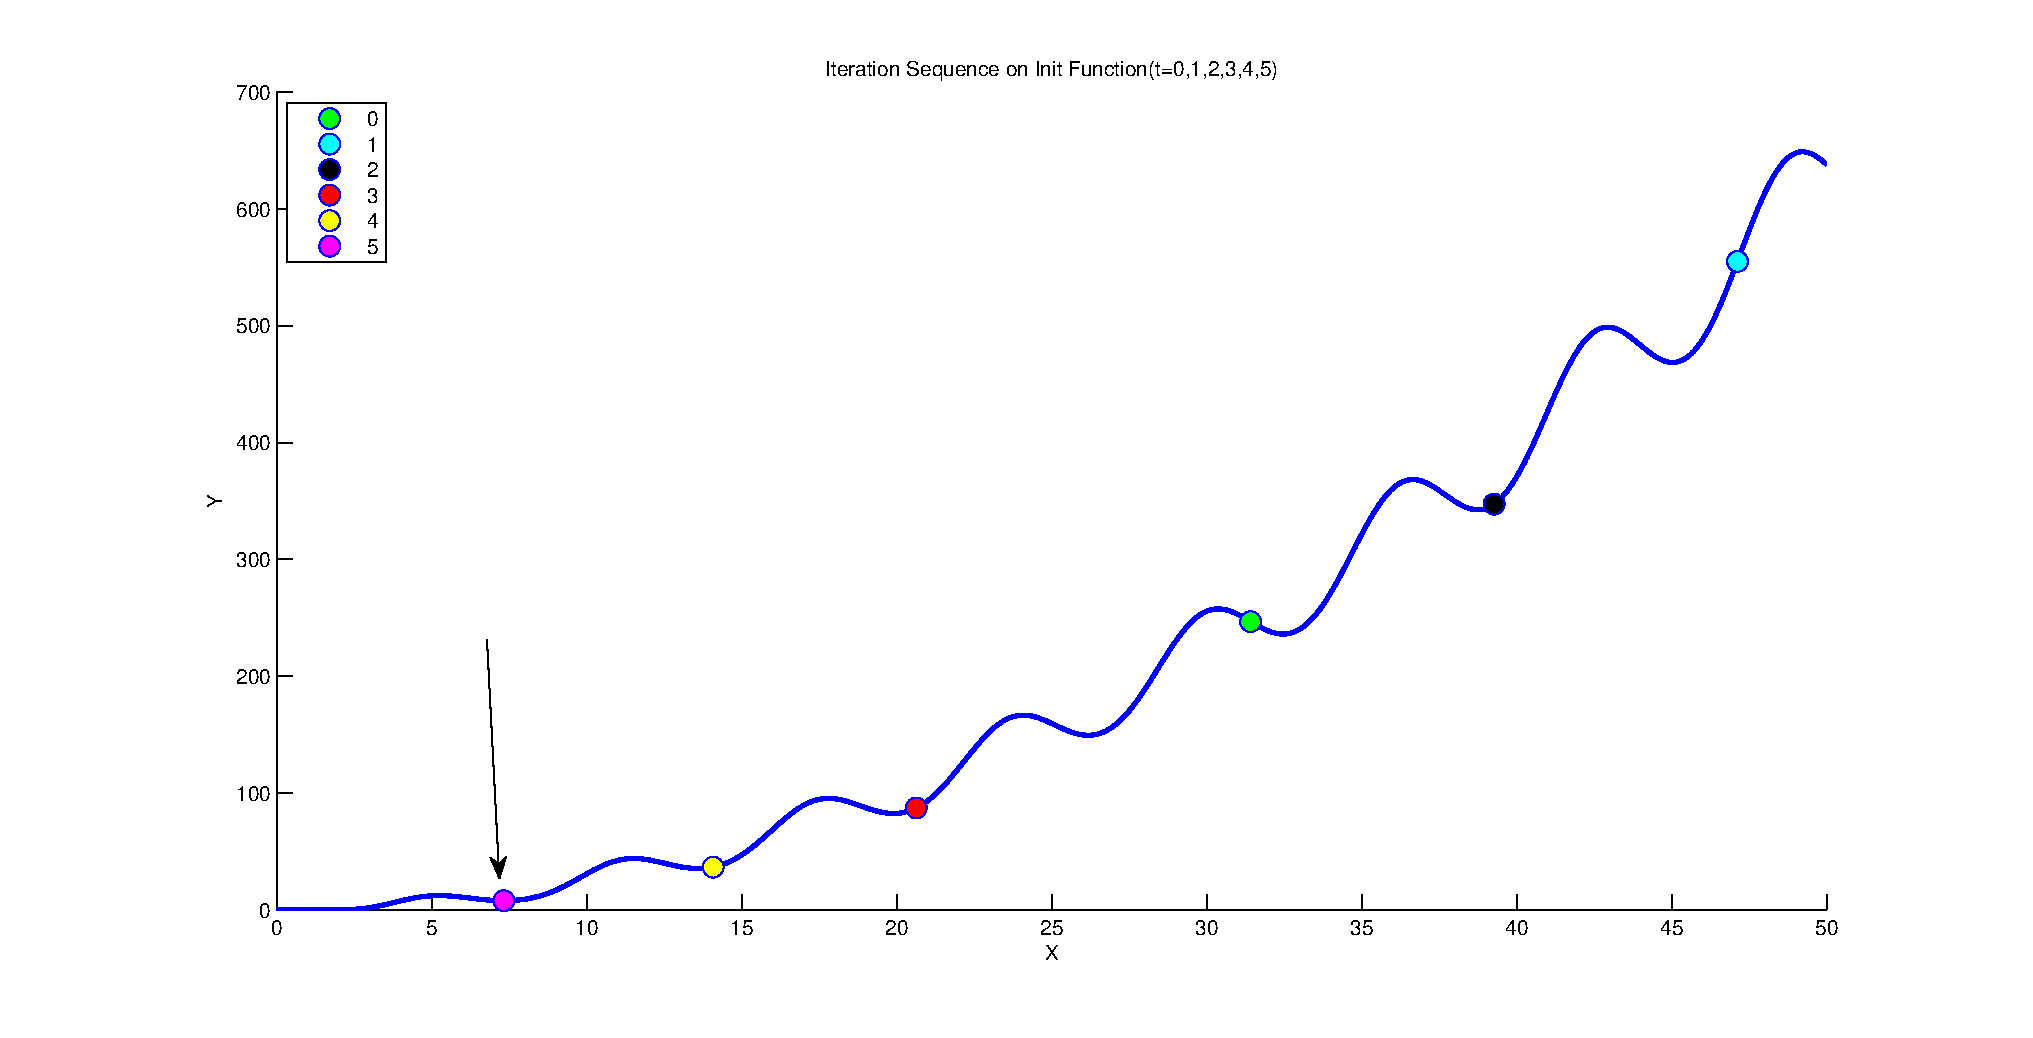
\includegraphics[width=1.0\textwidth]{../chapter2_3_5.eps}
					\caption{$x_0 = 10\pi$. 迭代点在函数图像上的分布($t = 0,1,2,3,4,5$). 注意到$t=5$时, 迭代点所处位置(箭头处), 函数导数约为$0$.}
					\label{img_chapter2_3_5}
				\end{figure}
			
				根据牛顿法迭代公式$x_n = x_{n-1} - \frac{f\left(x_{n-1} \right)}{f'\left(x_{n-1} \right)}$, 当在某一迭代点处, 导数约为$0$时, 下一次迭代数值将会很大, 这样将会导致不收敛或溢出的现象. 在本题中, $x_0=10\pi $时, 第6次迭代结果为$1.9215e+03$.
				
				本题函数有一定波动性, 使用牛顿法容易出现不收敛的情况. 观察结果可知, 如果给定的初始值比较靠近零点, 那么有利于牛顿法收敛. 当给定初始值偏离零点较远时, 容易出现不收敛的情况.
		\subsection{Problem 4}
			\paragraph{题目描述}
			:\newline
				已知$f\left(x\right) = 5x - e^x$在$\left(0,1\right)$之间有一个实根, 试分别利用二分法、牛顿法、割线法、错位法设计相应的计算格式, 并编程求解(精确到$4$位小数).
			
			\paragraph{分析}
			:\newline
				当$x \in \left[0,1 \right]$时, $f'\left(x\right) = 5 - e^x > 0$, 而$f\left(0 \right) = -1 < 0, f\left(1\right) = 5-e>0$. 因此$f\left(x\right)$在$\left[0,1 \right]$上有且仅有一个零点.
			
			\paragraph{二分法}
				:代码\newline
				\begin{lstlisting}[language=Matlab]
					f = @(x)5*x-exp(x);
					TOL = 5e-5; N = 100; Left = 0.0; Right = 1.0;
					FL = f(Left); A = [];
					X = Left:(Right - Left)/400:Right; Y = f(X);
					CNT = 0; Mid = 0;
					while CNT < N
						CNT = CNT + 1;
						Mid = (Left + Right)/2; FMid = f(Mid); A(CNT) = FMid;
						if FL*FMid < 0
							Right = Mid;
						else
							if FL*FMid == 0
								break
							else
								FL = FMid;
								Left = Mid;
							end
						end
						if Right - Left < TOL
							break
						end
					end
					subplot(1,2,1);
					plot(X,Y,Mid,FMid,'o',[Mid,Mid],[min(Y),max(Y)],'r:',[X(1),X(length(X))],[FMid,FMid],':r');
					title('Zero Point of Function')
					legend('2-3*x-sin(x)','Zero Point')
					subplot(1,2,2);
					plot(1:CNT,A,'o',1:CNT,A,'-r');
					title('Iteration Sequence of f(x)');
					legend('f(x) of each iteration')
					fprintf('Total time of iteration is %d. The answer is %.4f.',CNT,Mid)
				\end{lstlisting}
				\subparagraph{Output}
					Total time of iteration is $15$. The answer is $0.2592$.
					
					Graph:
					
					\begin{figure}[H]
						\centering
						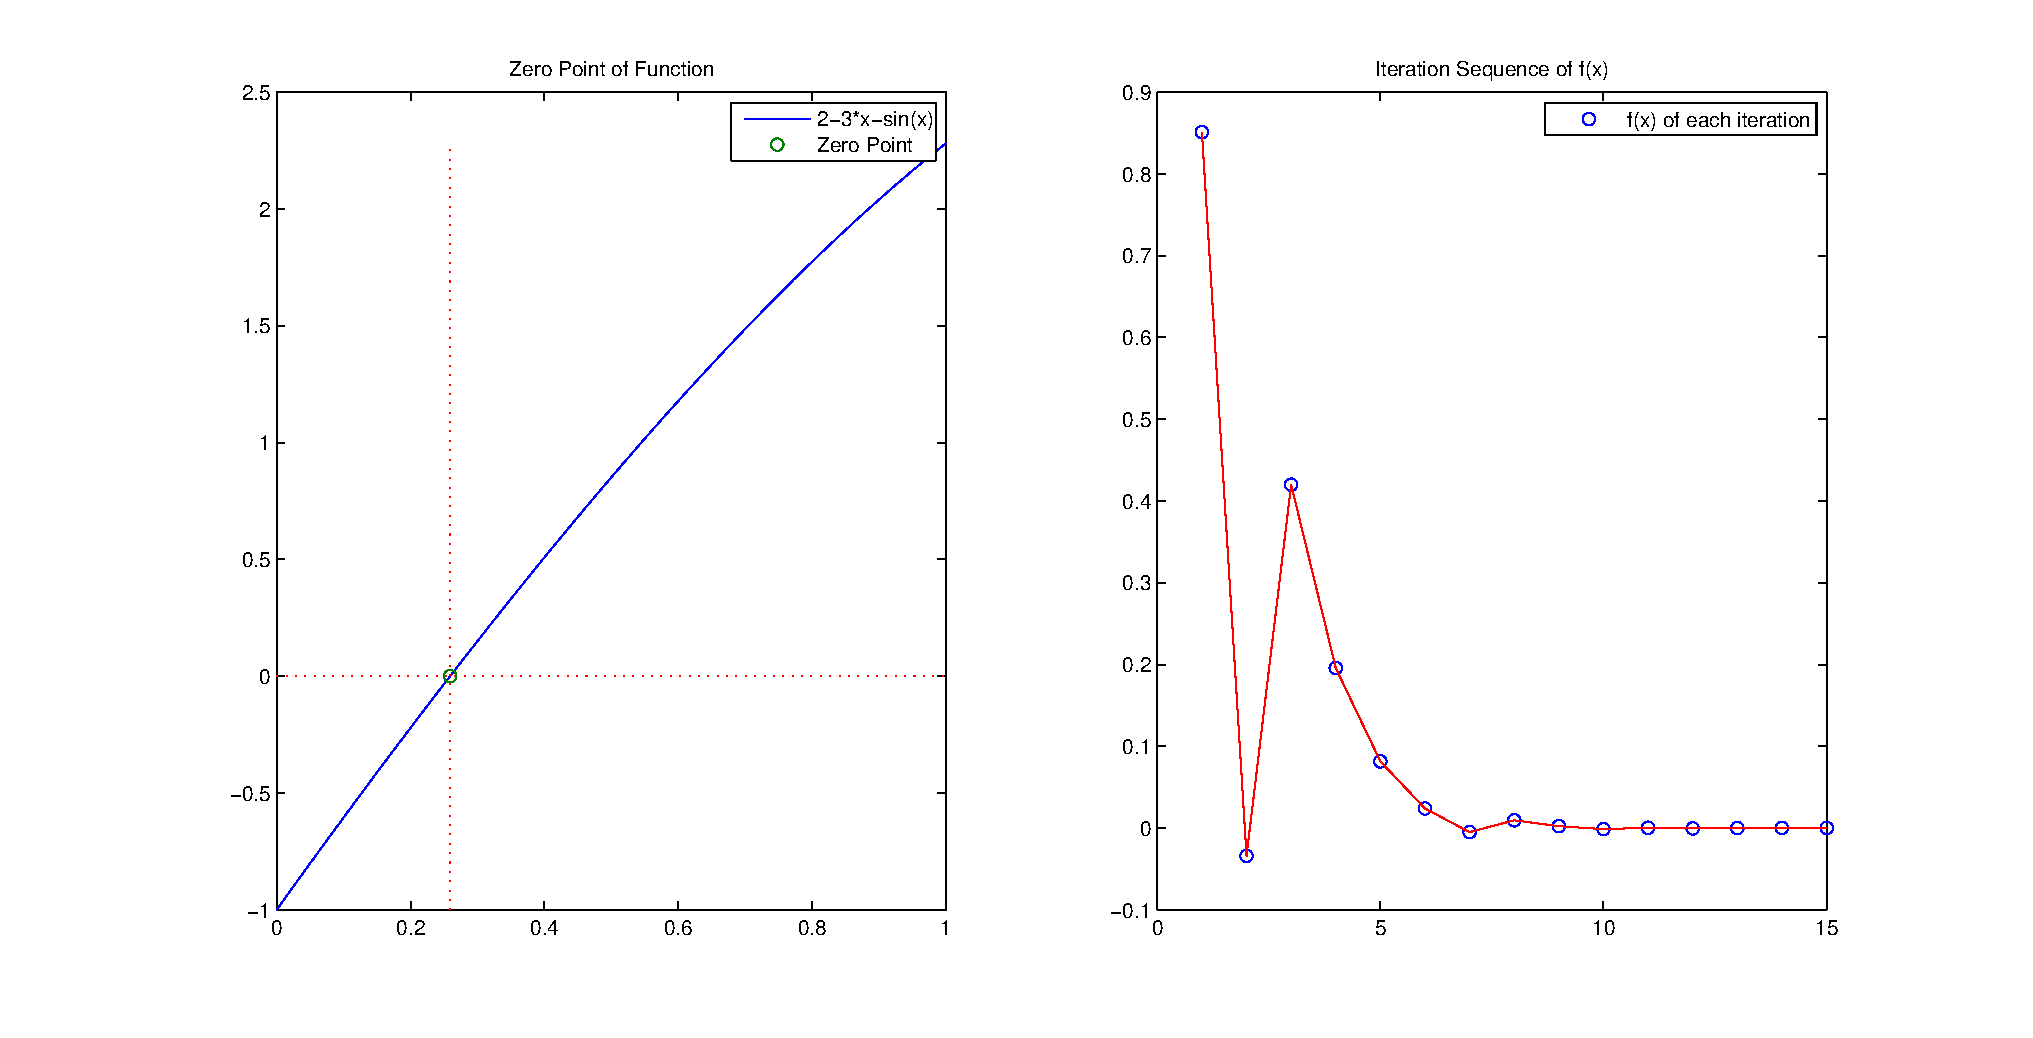
\includegraphics[width=1.0\textwidth]{../chapter2_4_1.eps}
						\caption{二分法迭代序列. 左图为函数零点, 右图为迭代$f\left(x\right)$序列}
						\label{img_chapter2_4_1}
					\end{figure}
			\paragraph{牛顿法}
				
				\subparagraph{代码}
				:\newline
					\begin{lstlisting}[language=Matlab]
						f = @(x)5*x-exp(x); diff_f = @(x)5-exp(x);
						Left = 0; Right = 1;                      
						TOL = 5e-5; N = 100; CNT = 1;
						x0 = 0; A = x0;
						while CNT < N
							CNT = CNT + 1;
							x = x0 - f(x0)/diff_f(x0);
							A(CNT) = x;
							if abs(x - x0) < TOL
								break;
							end
							x0 = x;
						end
						fprintf('Total time of iteration is %d. The answer is %f.',CNT,A(CNT))
					\end{lstlisting}
				\subparagraph{Output}
					Total time of iteration is $4$. The answer is $0.259171$.
					Graph:
					\begin{figure}[H]
						\centering
						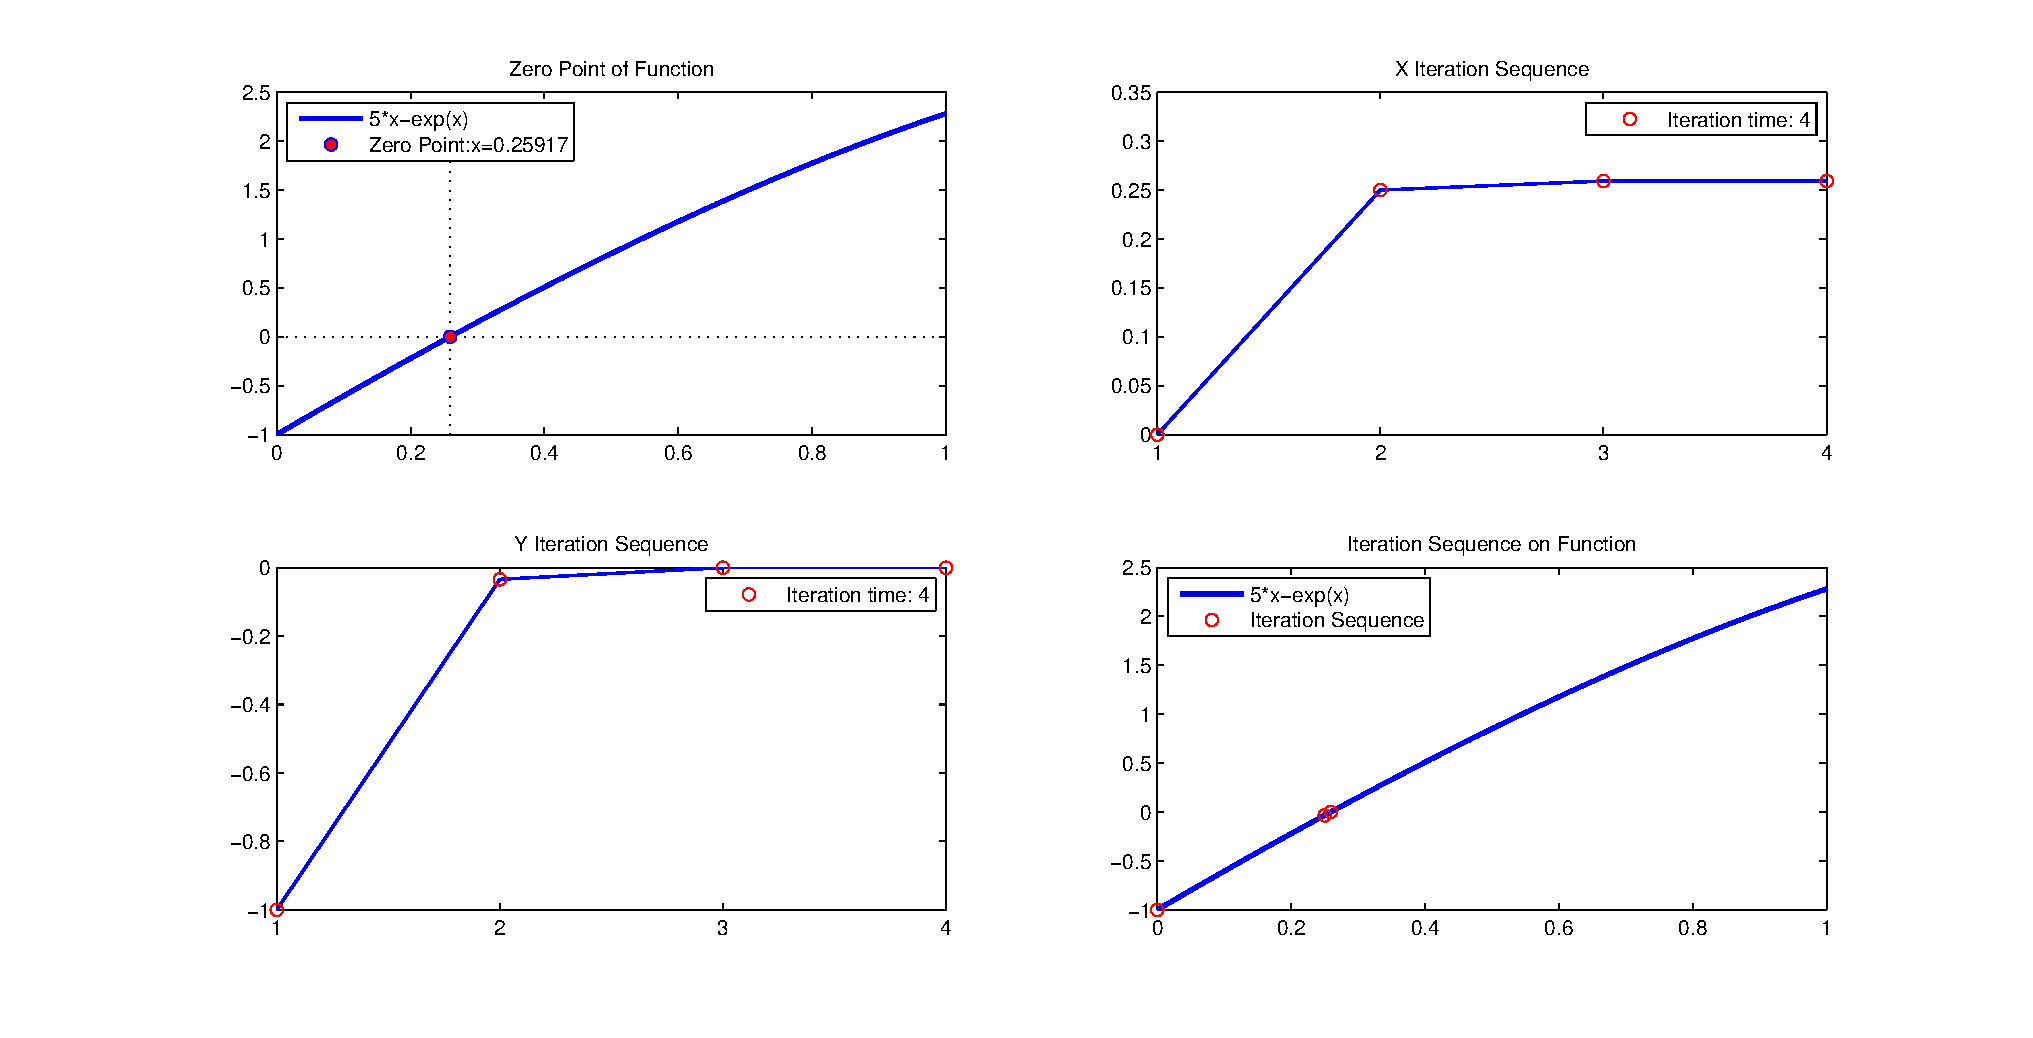
\includegraphics[width=1.0\textwidth]{../chapter2_4_2.eps}
						\caption{牛顿法迭代序列. 左上为函数零点, 右上为$x$迭代序列, 左下为对应$f\left(x\right)$序列, 右上为迭代点在函数图像上的分布}
						\label{img_chapter2_4_2}
					\end{figure}					
			\paragraph{割线法}
				\subparagraph{推导}
				: \newline
				用割线近似代替牛顿法中的切线.
				得到公式$x_{k+1} = x_k - f\left(x_k\right) \frac{x_k - x_{k-1}}{f\left(x_k\right) - f\left( x_{k-1}\right)}$.
				
				\subparagraph{代码}
				:\newline
					\begin{lstlisting}
					f = @(x)5*x-exp(x)
					Left = 0; Right = 1;
					TOL = 5e-5; N = 100; CNT = 1;
					x0 = Right; x1 = Left; A = x1;
					while CNT < N
						CNT = CNT + 1;
						x = x1 - f(x1)*(x1-x0)/(f(x1)-f(x0))
						A(CNT) = x;
						if abs(x - x1) < TOL
							fprintf('Total time of iteration is %d. The answer is %f.',CNT,x1);
							return;
						end
						x0 = x1; x1 = x;
					end
					disp('No Solution');
					\end{lstlisting}
				\subparagraph{Output}
				Total time of iteration is $5$. The answer is $0.259156$.\\
				Graph:\\
				\begin{figure}[H]
					\centering
					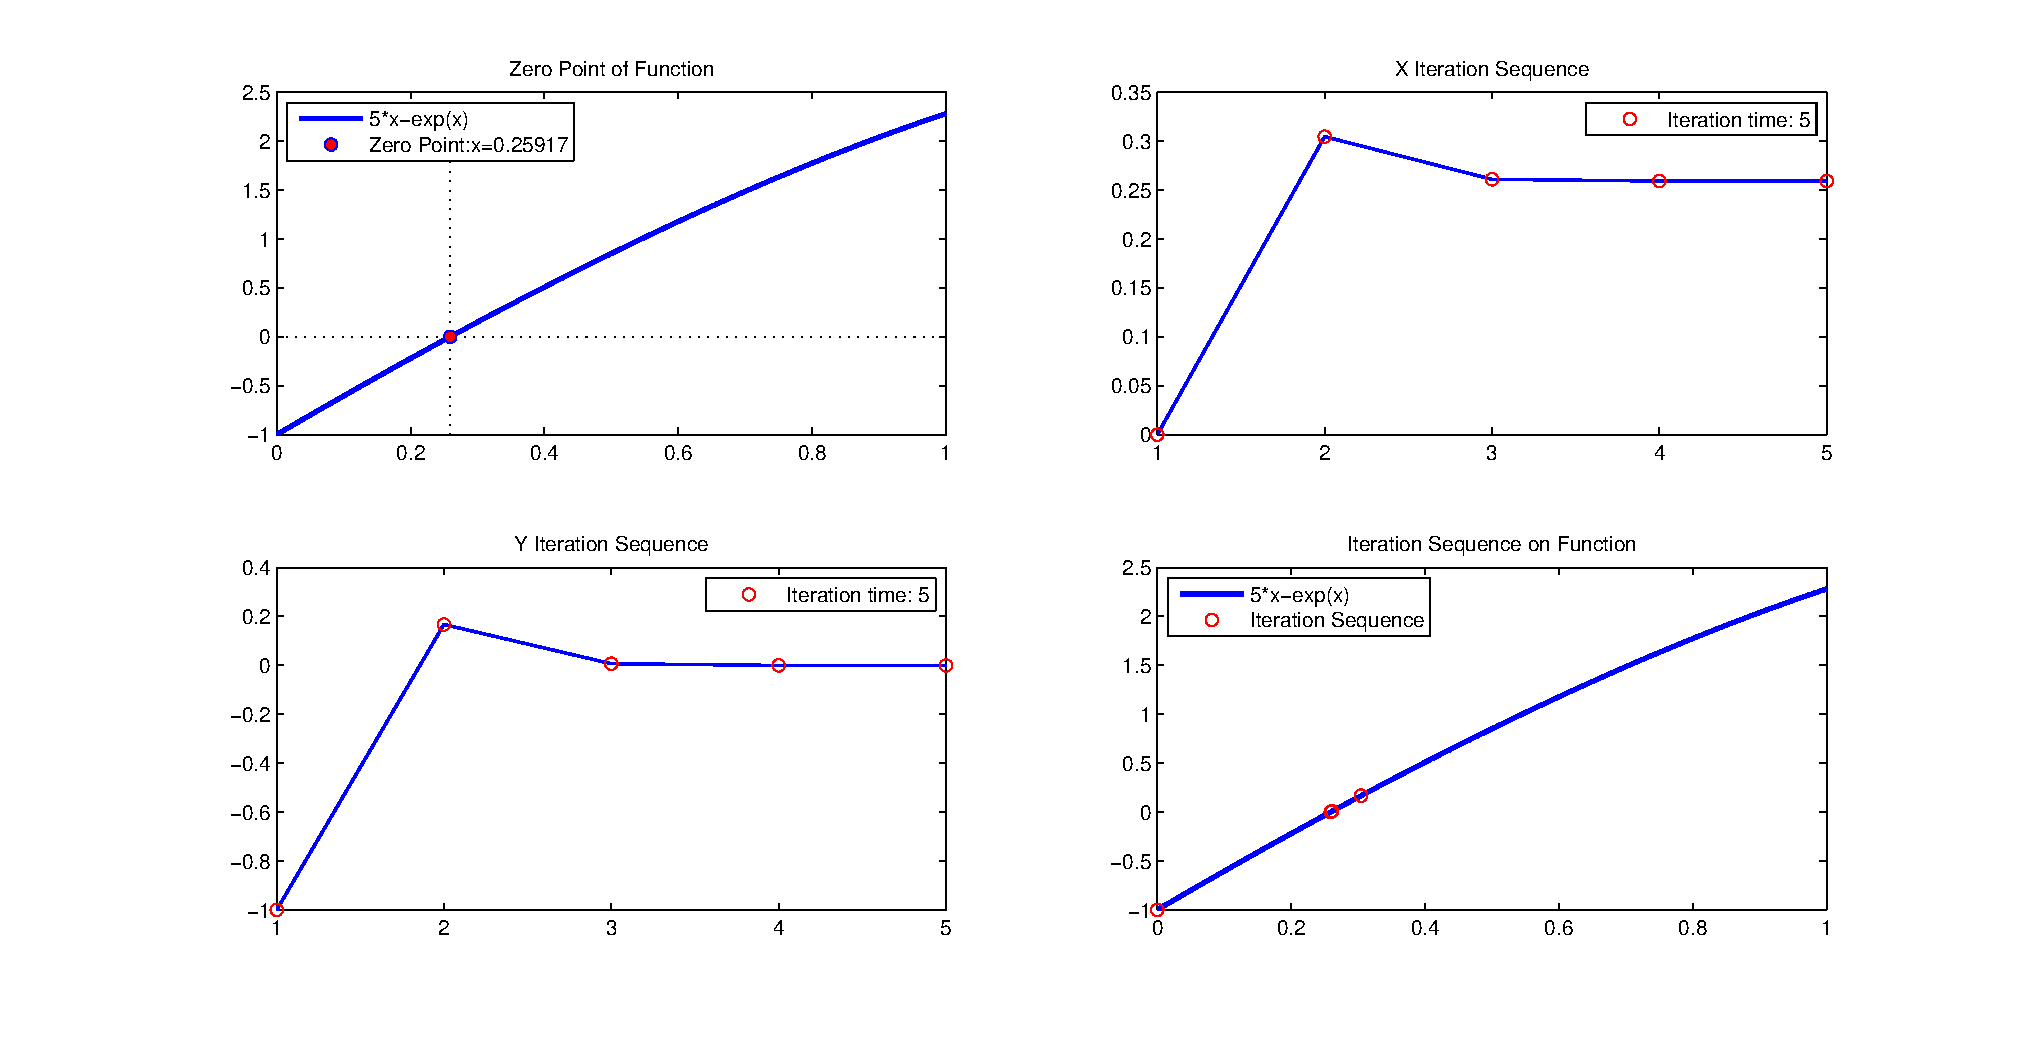
\includegraphics[width=1.0\textwidth]{../chapter2_4_3.eps}
					\caption{割线法迭代序列. 左上为函数零点, 右上为$x$迭代序列, 左下为对应$f\left(x\right)$迭代序列, 右下为迭代点在函数图像上的分布}
					\label{img_chapter2_4_3}
				\end{figure}
			\paragraph{错位法}
				\subparagraph{推导}
					:要在区间$\left[p_0,p_1 \right]$上寻找$f\left(x\right) = 0$的解, 其中$f\left(p_0 \right) f\left(p_1 \right) < 0$.
					
					使用与切线法相同的方式, 找到近似点$p_2$.
					
					为确定使用哪一条线计算$p_3$, 计算$f\left(p_2 \right) f\left(p_1 \right)$和$f\left( p_2\right) f\left(p_0 \right)$.
					
					如果$f\left(p_2 \right) f\left(p_1 \right) < 0$, 说明$p_1,p_2$中间包含了一个根, 那么取$\left(p_1,f\left(p_1\right) \right),\left(p_2,f\left(p_2 \right)\right)$线段的斜率, 作为切线法中的斜率.
				\subparagraph{代码}
					:\newline
					\begin{lstlisting}
					f = @(x)5*x-exp(x);
					Left = 0; Right = 1; TOL = 5e-5; N = 100; CNT = 1;
					p0 = Left; p1 = Right; q0 = f(p0); q1 = f(p1); A = p1;
					while CNT < N
						CNT = CNT + 1
						p = p1 - q1*(p1-p0)/(q1-q0); A(CNT) = p;
						if abs(p-p1) < TOL
							fprintf('Total time of iteration is %d. The answer is %f.',CNT,p);
							return
						end
						q = f(p)
						if q*q1 < 0
							p0=p; q0=q;
						else
							p1=p; q1=q;
						end
					end
					disp('No Solution')
					\end{lstlisting}
				\subparagraph{Output}
					Total time of iteration is $6$. The answer is $ 0.259171$.
					Graph:\\
					\begin{figure}[H]
						\centering
						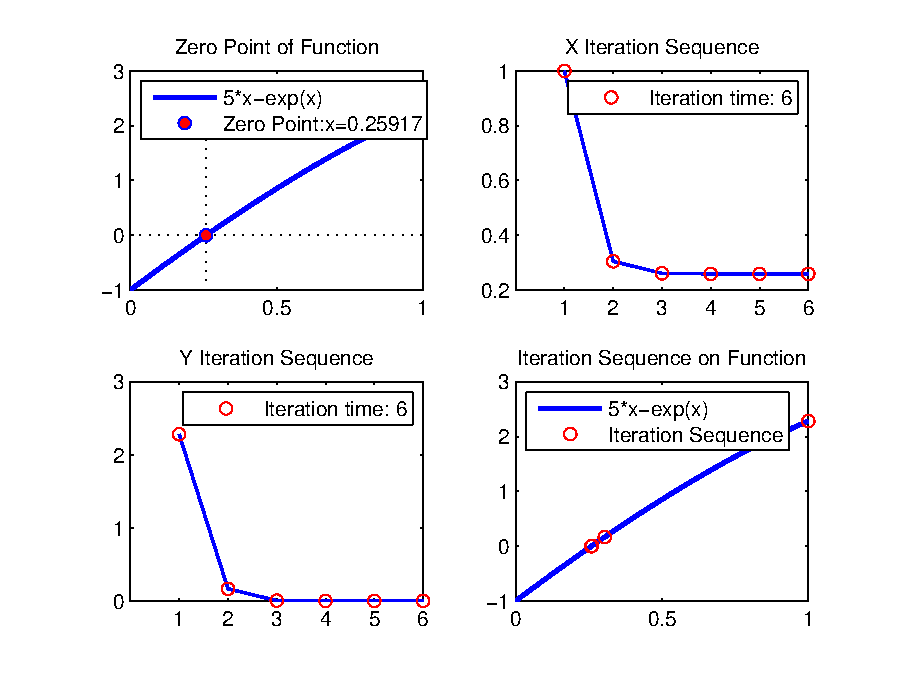
\includegraphics[width=1.0\textwidth]{../chapter2_4_4.eps}
						\caption{错位法迭代序列. 左上为函数零点, 右上为$x$迭代序列, 左下为对应$f\left(x\right)$迭代序列, 右下为迭代点在函数图像上的分布}
						\label{img_chapter2_4_4}
					\end{figure}
			\paragraph{画图代码}:\newline
				\begin{lstlisting}
					X = Left:(Right-Left)/400:Right; Y = f(X);
					B = f(A);
					subplot(2,2,1);
					plot([min(X),max(X)],[B(CNT),B(CNT)],':k',[A(CNT),A(CNT)],[min(Y),max(Y)],':k');
					hold on
					tmp1 = plot(X,Y,'LineWidth',2);
					tmp2 = plot( A(CNT),B(CNT), 'o', 'markerfacecolor', [ 1, 0, 0 ] );
					legend([tmp1,tmp2],'5*x-exp(x)',['Zero Point:x=' num2str(A(CNT))],2)                       
					title('Zero Point of Function');
					subplot(2,2,2);
					hold on;
					tmp3 = plot(1:CNT,A,'-b','LineWidth',1.2);
					tmp4 = plot(1:CNT,A,'or');
					set(gca,'xtick',1:CNT);
					legend(tmp4,['Iteration time: ' num2str(CNT)])
					title('X Iteration Sequence');
					subplot(2,2,3);
					hold on;
					tmp5 = plot(1:CNT,B,'-b','LineWidth',1.2);
					tmp6 = plot(1:CNT,B,'or');
					set(gca,'xtick',1:CNT);
					legend(tmp6,['Iteration time: ' num2str(CNT)])
					title('Y Iteration Sequence');
					subplot(2,2,4);
					hold on;
					tmp7 = plot(X,Y,'b','LineWidth',2);
					plot(A,B,'or');
					title('Iteration Sequence on Function');
					legend('5*x-exp(x)','Iteration Sequence',2);
				\end{lstlisting}
	\section{Chapter 3}
		\subsection{Problem 1}
		 	\paragraph{题目描述}
		 		:\newline 
		 		利用函数$y=\frac{1}{1+x^2}$, $x \in \left[-5,5\right]$生成相应的网格点数据, 分别取$n=2,4,6,8,10$, 画出该函数在$\left[-5,5\right]$上的$n$次拉格朗日多项式函数图形, 并与原函数图形比较, 分析插值多项式的次数对插值计算结果的影响.
		 	\paragraph{拉格朗日插值多项式}
		 		对于给定的$n+1$个点, $n$次拉格朗日插值多项式以此通过这$n+1$个点.
		 		
		 		拉格朗日多项式形式如下:
		 		$$P\left(x\right) = \sum_{k=0}^{n}L_{n,k}\left(x\right) f\left(x\right)$$.
		 		
		 		其中$L_{n,k}\left(x\right)$为基函数, 满足这样的性质:
		 		$$L_{n,k}\left(x_i\right)=\left\{
		 			\begin{aligned}
		 				0, \ i \neq k \\
		 				1, \ i = k
		 			\end{aligned}
		 		 \right.$$
		 		 
		 		取$$L_{n,k}\left(x\right) = \prod_{i=0,i \neq k}^{n} \frac{x-x_i}{x_k - x_i}$$.
		 	\paragraph{拉格朗日余项}
		 		$f\left(x\right) = P\left(x\right) + R\left(x \right)$, 其中$P\left(x\right)$为$n$次多项式, $$R\left(x\right) = \frac{f^{\left(n+1\right)}\left(\xi\left(x\right)\right)}{\left(n+1\right)!}\prod_{i=0}^{n}\left(x-x_i\right)$$为余项. 用于误差估计.
		 		
		 	\paragraph{Code \& Output}
		 	:\newline
		 		拉格朗日插值:
		 		\begin{lstlisting}
		 			function yy=lagrange(x1,y1,xx)  
		 				syms x  
		 				n=length(x1);  
		 				for i=1:n  
		 					t=x1;t(i)=[];L(i)=prod((x-t)./(x1(i)-t)); 
		 				end  
		 				u=sum(L.*y1);  
		 				yy=double(subs(u,x,xx));
		 			end  
		 		\end{lstlisting}
		 		
		 		对$y=\frac{1}{1+x^2}$处理、画图
		 		\begin{lstlisting}
		 			clear
		 			f = @(x)1/(1+x*x);
		 			left = -5; right = 5;
		 			X=left:(right-left)/200:right;
		 			P = [];
		 			for n=2:2:10
		 				step = (right - left) / n;
		 				A = left:step:right; B = [f(left)];
		 				for l = 1:n
		 					B(l+1) = f(A(l+1));
		 				end
		 				P = [P;lagrange(A,B,X)];
		 			end
		 			Y0=[];
		 			for l = 1:length(X)
		 				Y0(l) = f(X(l));
		 			end
		 			plot(X,Y0,X,P(1,:),X,P(2,:),X,P(3,:),X,P(4,:),X,P(5,:))
		 			legend('Initial Function','Lagrange function:2th','4th','6th','8th','10th');
		 		\end{lstlisting}
		 		\begin{figure}[H]
		 			\centering
		 			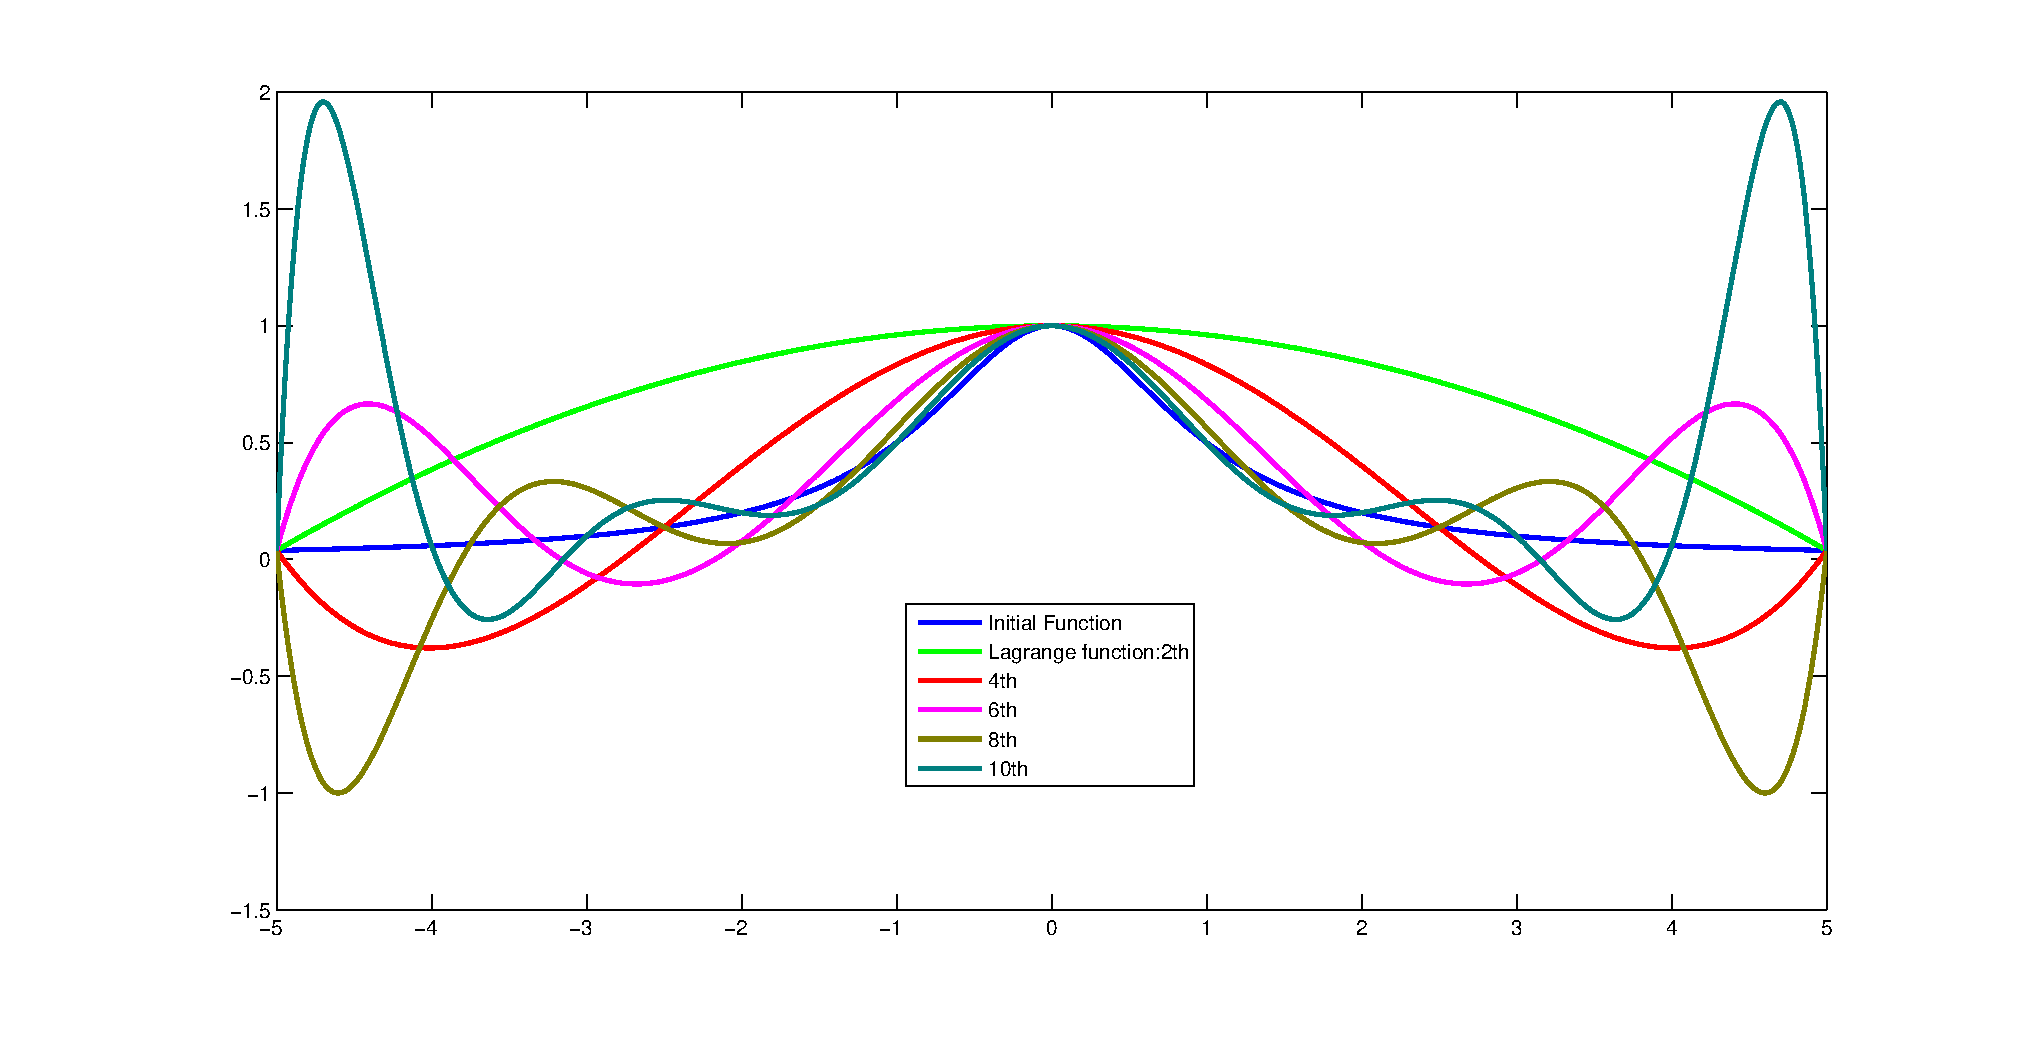
\includegraphics[width=1.0\textwidth]{../chapter3_1.eps}
		 			\caption{插值曲线与原始函数比较. 包括了原始函数、$2,4,6,8,10$次插值多项式}
		 			\label{img_chapter3_1}
		 		\end{figure}
	 			
	 			\begin{figure}[H]
	 				\centering
	 				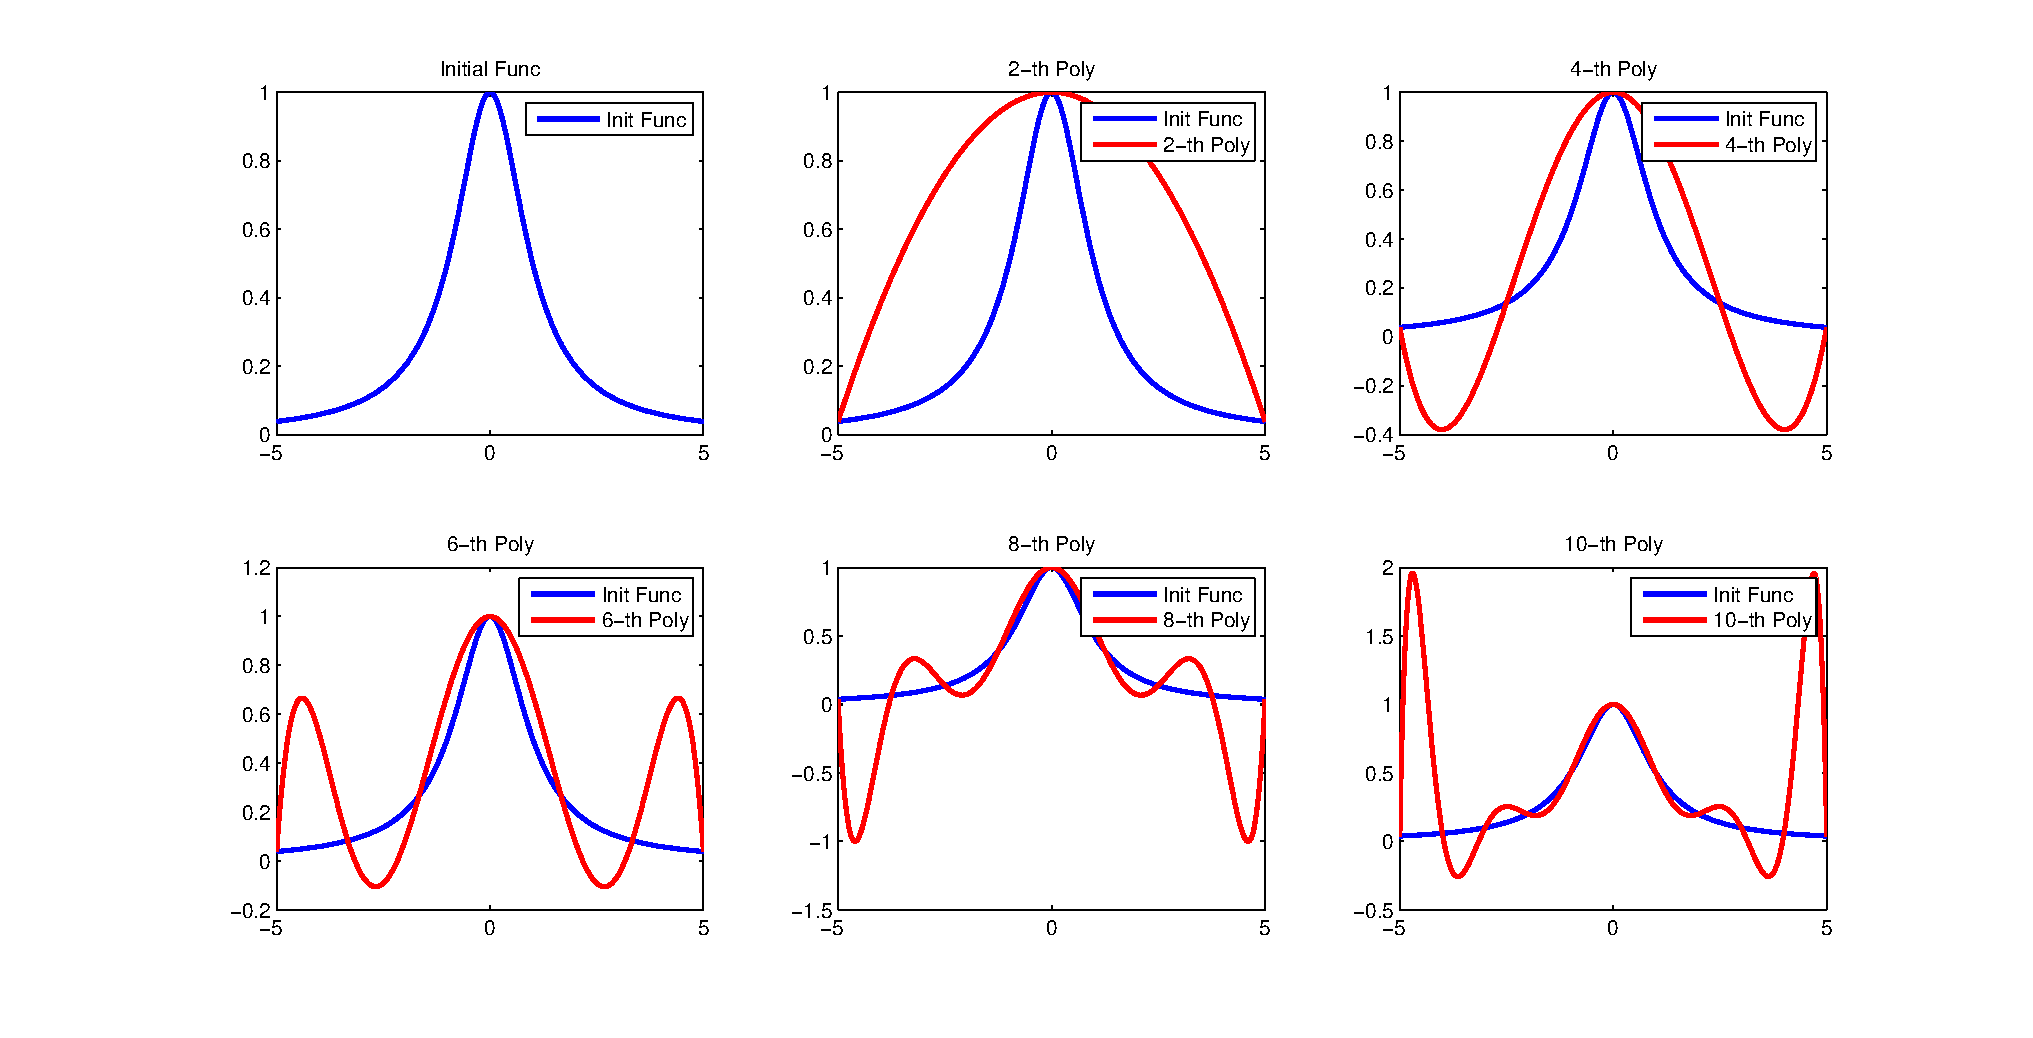
\includegraphics[width=1.0\textwidth]{../chapter3_1_tot.eps}
	 				\caption{插值曲线与原始函数比较. 分别为原始函数、$2,4,6,8,10$次多项式}
	 				\label{img_chapter3_1_tot}
	 			\end{figure}
 			\paragraph{分析}:\newline
 				误差分析:\\
 				\begin{tabular}{|c|c|c|c|c|c|}
 					\hline
 					 $n$-th Lagrange Poly & 2 & 4 & 6 & 8 & 10\\
 					\hline
 					$\max \left| f^{\left(n+1\right)}\left(\xi\right) \right| $ & 4.6686 &100.4528 & 4.3910e+03& 3.2423e+05 &  3.6289e+07\\
					\hline
					$\max\left|\prod_{i=0}^{n}\left(x-x_i\right) \right| $ & 48.1124
					 & 354.6317 & 3.4236e+03 & 3.6722e+04 & 4.1655e+05 \\
 					\hline 
 					$\left| R\left(x\right)\right|$上界 &37.4363 &296.8646 &2.9827e+03& 3.2811e+04 &3.7869e+05 \\
 					\hline
 					$\max \left|R\left(x\right) \right|$& 0.6462 & 0.4383 & 0.6169 & 1.0452 & 1.9156 \\
 					\hline
 				\end{tabular}
 			
 				对于此问题, 用给定的$R\left(x\right)$表达式来估算误差上界, 效果不好. 原因在于$\left|f^{\left(n+1\right)}\left(\xi\right) \right|$在$n$较大时, 在个别点取值较大, 从而影响了$\inf \left|f^{\left(n+1\right)} \left(x\right) \right|$取值. 在本题实际情况下, 往往取不到上界.
 				
 				龙格现象:\\
 				误差项中含有多项式:$\prod_{i=0}^{n}\left(x-x_i\right) $. 对于该多项式, 绘图如下:
 				\begin{figure}[H]
 					\centering
 					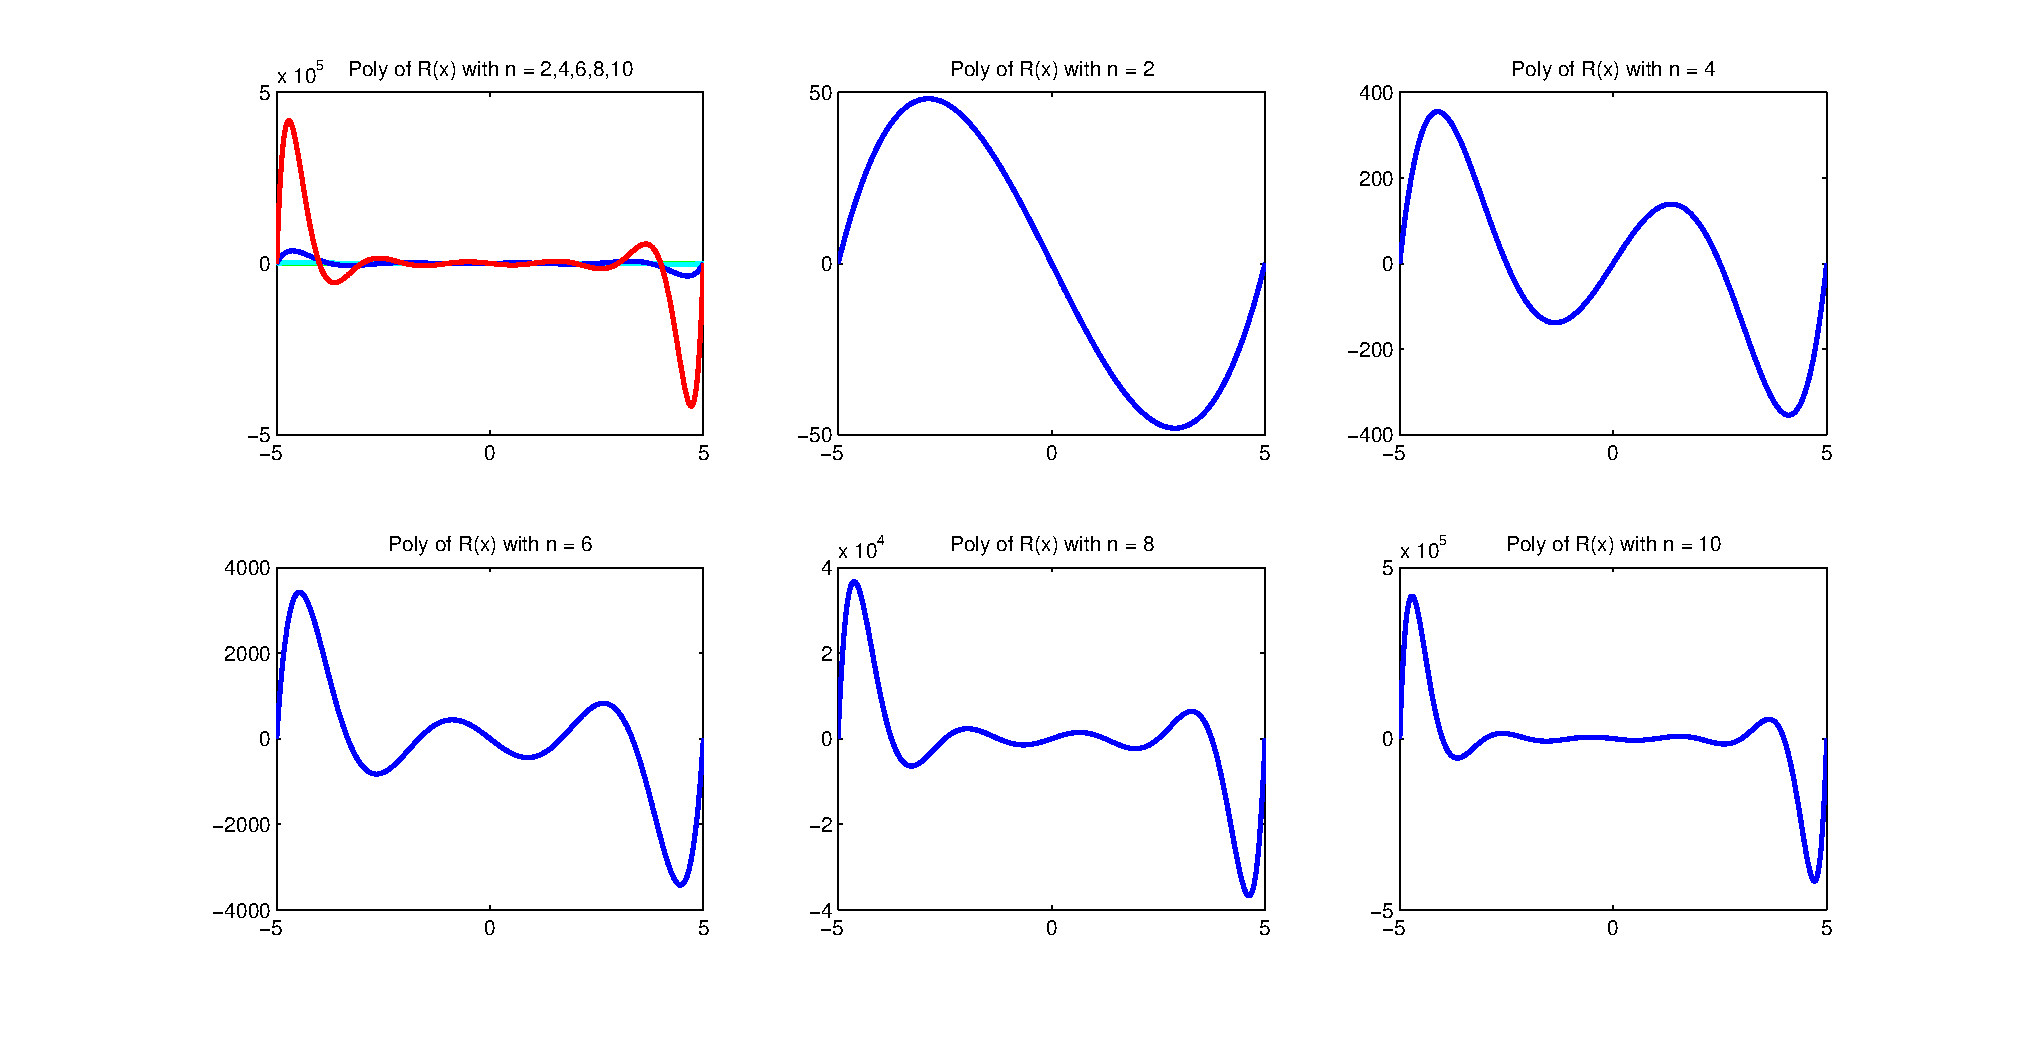
\includegraphics[width=1.0\textwidth]{../chapter3_1_lunge.eps}
 					\caption{误差项多项式比较. 左上为$2,4,6,8,10$次多项式总体比较. 之后依次是$2,4,6,8,10$次多项式}
 					\label{img_chapter3_1_lunge}
 				\end{figure}
 				从图中可以发现, 当$x$偏离中心时, 多项式绝对值较大. 此为龙格现象发生的原因.
 				\subparagraph{结论}
 				\begin{enumerate}
 					\item 当拉格朗日插值多项式次数较小的时候, 由于采样点数目较少, 插值多项式不能很好地贴合原始函数.
 					\item 当多项式次数较大时, 在插值区间的边界部分插值函数会出现很大波动, 明显偏离原始函数(龙格现象); 其次, 从舍入误差看, 高次插值由于计算量大, 可能会产生严重的误差积累, 稳定性得不到保障. 所以拉格朗日插值次数不宜过高.
 				\end{enumerate}

	\section{Chapter 4}
		\subsection{Problem 1}
			\paragraph{题目描述}
			:\newline
			计算积分$I\left(x\right) = \int_{0}^{\frac{\pi}{2}} e^{\sin x}dx$的数值解:
			\begin{enumerate}
				\item 分别取$h=\frac{\pi}{8000}, \frac{\pi}{800}, \frac{\pi}{80}$, 用复合梯形格式计算其数值积分计算结果, 观察$h$的大小对计算结果的有效数字和绝对误差的影响.
				\item 用辛普森公式重复上述计算过程.
				\item 将计算结果的绝对误差与理论误差比较, 验证理论结果的正确性.
			\end{enumerate}
		
			\paragraph{Question 1}
				\subparagraph{梯形法简介}:
					把被积区间划分成若干小区间, 对于每一小区间, 用函数两个端点与$x$轴围成的梯形面积, 近似代替函数图像与$x$轴围成的面积. 将所有小梯形面积累加, 即为结果.(或者说, 每一个小区间都用线性拉格朗日插值多项式来代替).
					
					积分公式可以表述为:
					$$f\left(x \right) dx = \frac{h}{2}\left[ f\left(a\right) + 2\sum_{j}^{n-1}f\left(x_j\right) + f\left(b\right)\right] - \frac{b-a}{12}h^2f^{''}\left(\mu\right)$$
					\begin{figure}[H]
						\centering
						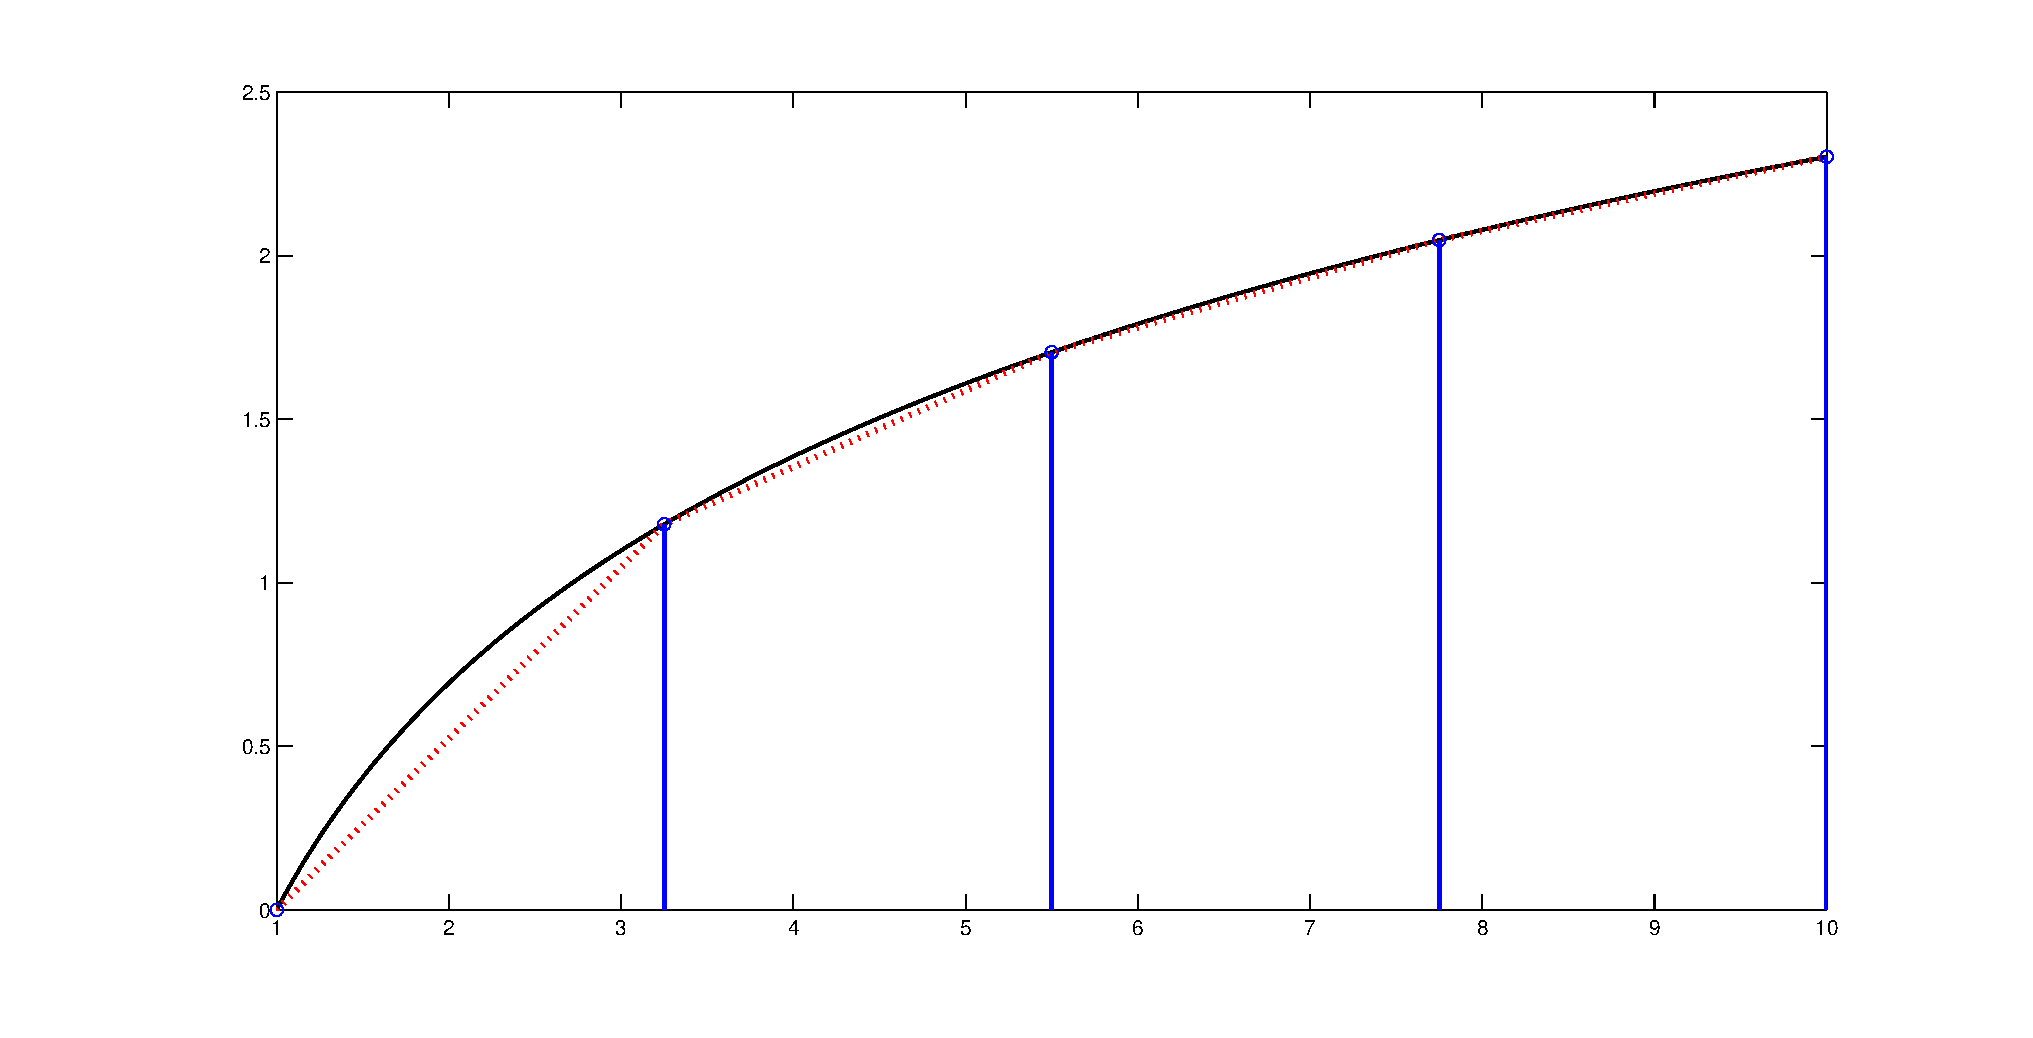
\includegraphics[width=1.0\textwidth]{../chapter4_1_txf.eps}
						\caption{梯形法图示}
						\label{img_chapter4_1_txf}
					\end{figure}
				\subparagraph{Code}
				:\newline
					\begin{lstlisting}
						left = 0; right = pi/2; h = pi/8000;
						f = @(x)exp(sin(x));
						tot = 0; tp = f(left);
						for i=left+h:h:right
						tr = f(i);
						tot = tot + h/2*(tp + tr);
						tp = tr;
						end
						fprintf('ans = %f\n',tot)
					\end{lstlisting}
				\subparagraph{Answer}
					\begin{enumerate}
						\item $h = \frac{\pi}{8000}$, $Ans = 3.104379$.
						\item $h = \frac{\pi}{800}$, $Ans = 3.104378$.
						\item $h = \frac{\pi}{80}$, $Ans = ans = 3.104251$.
					\end{enumerate}
				\subparagraph{Analysis}
					在$\left[0,\frac{\pi}{2}\right]$上, 
					令$f\left(x\right) = e^{\sin x}$, 则$f'\left(x\right) = e^{\sin x} \cos x > 0$,
					$f^{''}\left(x\right) = e^{\sin x} \cos^2 x - e^{\sin x}\sin x$. 有$\max \left| f^{''}\left(x\right)\right| = f^{''}\left(1\right) \approx  -1.2748$.
					
					因此误差项$\left|\frac{b-a}{12}h^2f^{''}\left(\mu\right) \right| = \left| \frac{\pi /2 *h^2}{12}f^{''}\left(\mu\right)\right| \leq \left|\frac{\pi /2 *h^2}{12} f^{''}\left(1\right) \right|$
					
					代入不同的$h$, 可以得到:
					\begin{center}
						\begin{tabular}{|c|c|c|c|}
							\hline
							$h$    & $\pi /80$ &$\pi /800$ & $\pi /8000$ \\
							\hline
							$ \left|\frac{\pi /2 *h^2}{12} f^{''}\left(1\right) \right| $ & 2.5734e-04
							& 2.5734e-06 & 2.5734e-08\\
							\hline
						\end{tabular}
					\end{center}
					
			\paragraph{Question 2}
				\subparagraph{辛普森公式推导}
				:\newline
					设$x_1 = x_0 + h, x_2 = x_0 + 2h\left(h>0\right)$
					$\forall x \in \left[x_0,x_2 \right]$,$\exists \xi \left(x \right) \in \left[x_0,x_2 \right]$, 使得
					$$f\left(x\right) = f\left(x_1\right) + f'\left(x_1\right)\left(x-x_1\right) + \frac{f^{''}\left(x_1\right)}{2}\left(x-x_1\right)^2 +$$
					
					$$ \frac{f^{'''}\left(x_1\right)}{6}\left(x-x_1\right)^3 + \frac{f^{\left(4\right)}\left(\xi\left(x\right)\right)}{24}\left(x-x_1\right)^4$$.
					积分, 得
					$\int_{x_0}^{x_2}f\left(x\right)dx = $
					
					$$\left[f\left(x_1\right)\left(x-x_1\right) + \frac{f^{'}\left(x_1\right)}{2}\left(x - x_1\right)^2 + \frac{f^{''}\left(x_1\right)}{6}\left(x - x_1\right)^3 + \frac{f^{'''}\left(x_1\right)}{24}\left(x-x_1\right)^4 \right]_{x_0}^{x_2}$$
					
					$$
					 + \frac{1}{24} \int_{x_0}^{x_2} f^{\left(4\right)}\left( \xi \left(x\right)\right)\left(x-x_1\right)^4 dx$$
					 
					 由于$\forall x \in \left[x_0,x_2\right],\left(x-x_1\right)^4 \geq 0$, 因此
					 $$ \frac{1}{24} \int_{x_0}^{x_2} f^{\left(4\right)}\left( \xi \left(x\right)\right)\left(x-x_1\right)^4 dx = \frac{f^{\left(4\right)}\left(\xi_1\right)}{24} \int_{x_0}^{x_2} \left(x-x_1\right)^4 dx = 
					 \frac{f^{\left(4\right)}\left(\xi_1\right)}{120}\left(x-x_1\right)^5 |_{x_0}^{x_2}$$
					 其中$\xi_1 \in \left( x_0,x_2\right)$.
					 
					 利用$h=x_2 - x_1 = x_1 - x_0$, 上述积分表述为
					 $$ \int_{x_0}^{x_2} f\left(x\right) dx = 2hf\left(x_1\right) + \frac{h^3}{3}f^{''}\left(x_1\right) + \frac{f^{\left(4\right)\left(\xi_1 \right)}}{60}h^5$$.
					 
					 对于$f^{''}\left(x_1\right)$, 用如下方式处理:
					 $$f\left(x_0+h\right) = f\left(x_0\right) + f^{'}\left(x_0\right)h + \frac{1}{2}f^{''}\left(x_0 \right) h^2 + \frac{1}{6} f^{\left(3\right)}\left(x_0\right)h^3 + \frac{1}{24}f^{\left(4\right)}\left(\xi_1\right)h^4$$.
					 
					 $$f\left(x_0+h\right) = f\left(x_0\right) - f^{'}\left(x_0\right)h + \frac{1}{2}f^{''}\left(x_0 \right) h^2 - \frac{1}{6} f^{\left(3\right)}\left(x_0\right)h^3 + \frac{1}{24}f^{\left(4\right)}\left(\xi_1\right)h^4$$.
					 两式相加,
					 $$ f\left(x_0 + h\right) + f\left(x_0 - h\right) = 2f\left(x_0\right) + f^{''}\left(x_0\right) h^2 + \frac{h^4}{24}\left[f^{\left(4\right)}\left(\xi_1\right) + f^{\left(4\right)}\left(\xi_{-1}\right)\right]$$
					 取$f^{\left(4\right)}\left(\xi\right) = \frac{1}{2}\left[f^{\left(4\right)}\left(\xi_1\right) + f^{\left(4\right)}\left(\xi_{-1}\right)\right]$, 把$f^{''}\left(x_1\right)$的值代入, 可以求得
					 $$\int_{x_0}^{x_2}	f\left(x\right) dx = \frac{h}{3}\left[f\left(x_0\right) + 4f\left(x_1\right) +f\left(x_2\right) \right] - \frac{h^5}{12} \left[\frac{1}{3} f^{\left(4\right)} \left(\xi_2\right) - \frac{1}{5}f^{\left(4\right)}\left(\xi_1\right)\right]$$
					 余项可以写成$\frac{h^5}{90}f^{\left(4\right)}\left(\xi\right)$的形式.
					 
					 对于复合辛普森公式, 
					 $$\int_{a}^{b} f\left(x\right) dx = \sum_{j=1}^{n/2}\int_{x_{2j-2}}^{x_{2j}}f\left(x\right)dx =$$
					 
					 $$ \frac{h}{3}\left[f\left(x_0\right) + 2\sum_{j=1}^{n/2-1}f\left(x_{2j}\right) + 4\sum_{j=1}^{n/2}f\left(x_{2j-1} + f\left(x_n\right)\right)\right] + E\left(f\right)$$
					 
					 其中$E\left(f\right) = -\frac{h^5}{90} \sum_{j=1}^{n/2}f^{\left(4\right)}\left(\xi_j\right) = -\frac{b-a}{180}h^4f^{\left(4\right)}\left(\mu\right)$
					 
					 辛普森公式实质:
					 相邻的3个点用二次多项式进行插值, 误差项可以用上述方式推导.
					 
					 辛普森公式图示:
					 
					 \begin{figure}[H]
					 	\centering
					 	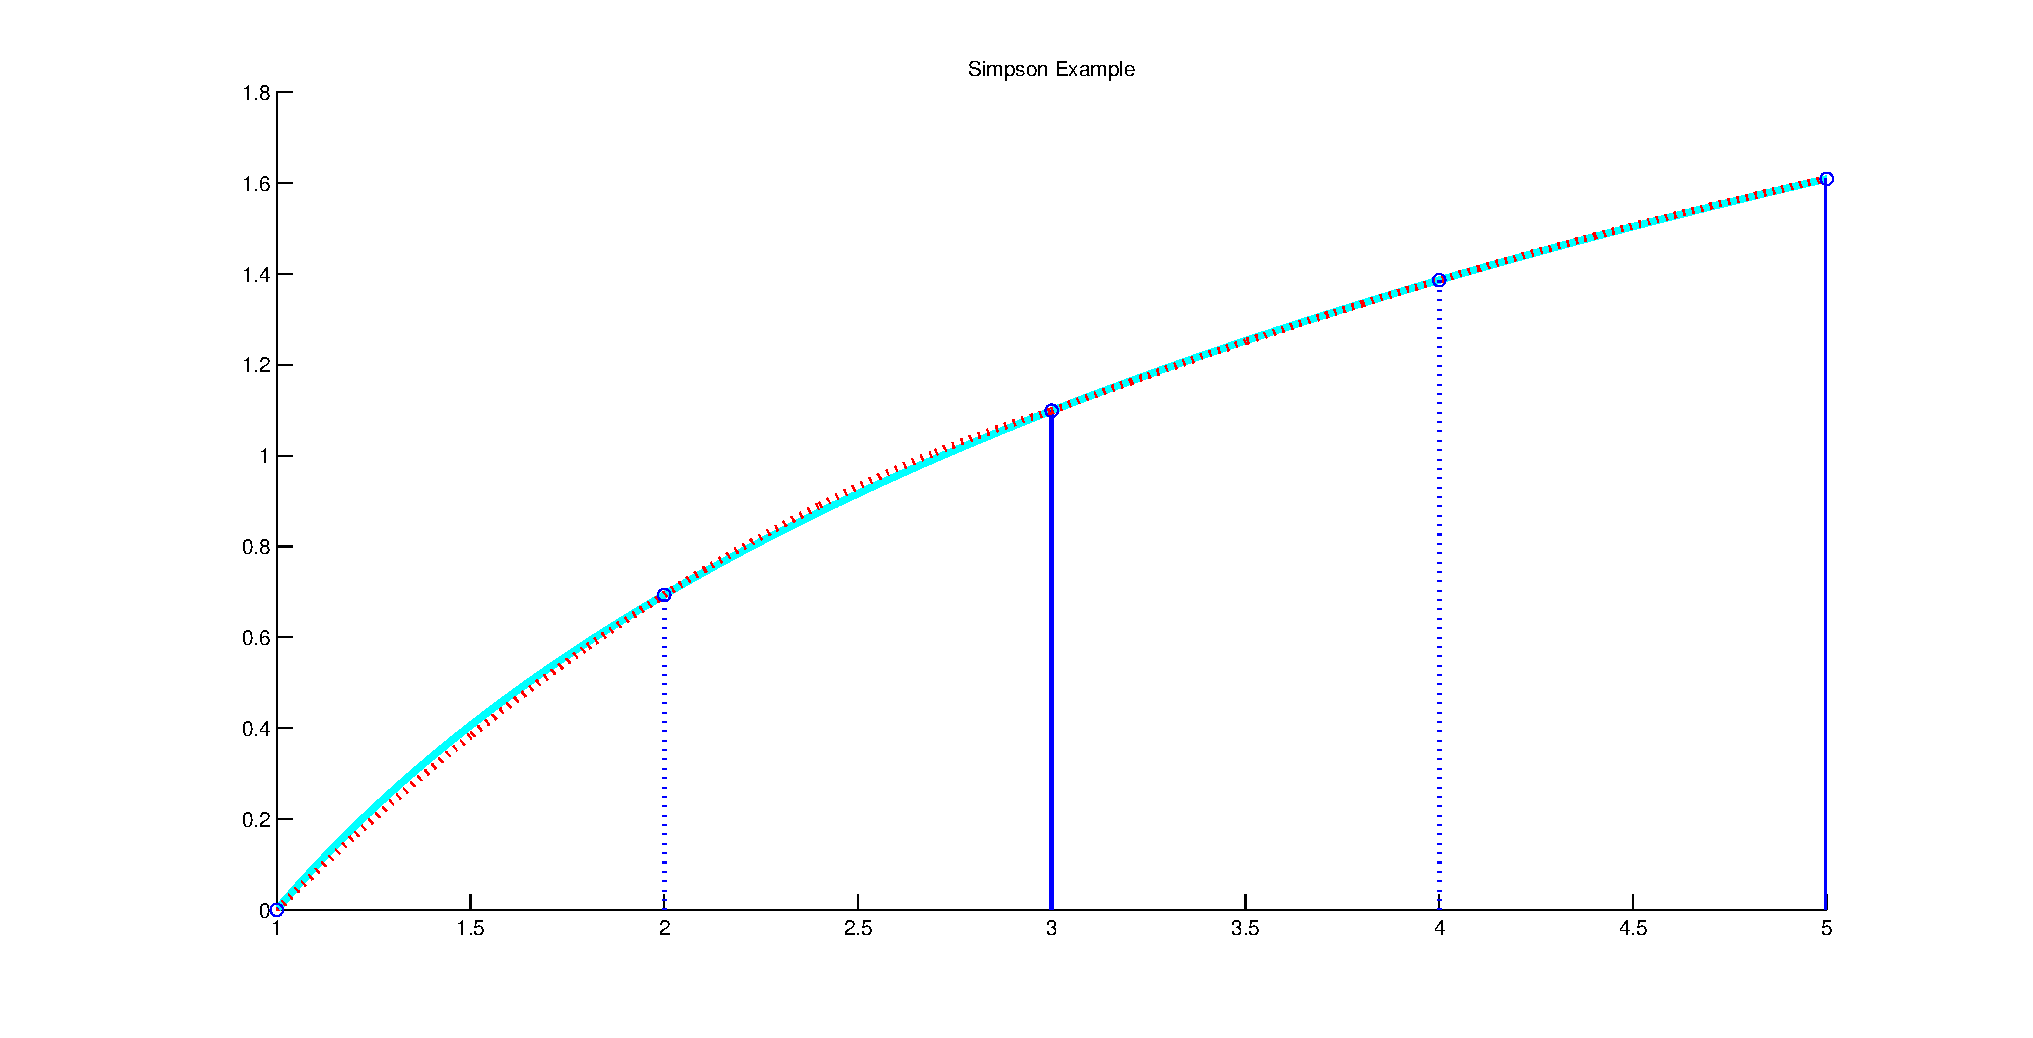
\includegraphics[width=1.0\textwidth]{../chapter4_simpson_ts.eps}
					 	\caption{辛普森公式图示}
					 	\label{img_chapter4_simpson_ts}
					 \end{figure}
					 
				\subparagraph{Code \& Answer}
				:\newline
					\begin{lstlisting}
						clear;
						f = @(x)exp(sin(x));
						left = 0; right = pi/2;
						n = 4000; h = (right - left) / n;
						tot = f(left) + f(right);
						for j=1:n/2-1
							tot = tot + 2*f(left + 2*j*h);
						end
						for j=1:n/2
							tot = tot + 4*f(left + (2*j-1)*h);
						end
						fprintf('ans = %f\n',h*tot/3)
					\end{lstlisting}
					
					\begin{enumerate}
						\item $h = \frac{\pi}{8000}$, $Ans = 3.104379017856$;
						\item $h = \frac{\pi}{800}$, $Ans = 3.104379017856$;
						\item $h = \frac{\pi}{80}$, $Ans = 3.104379017836$.
					\end{enumerate}
				\subparagraph{Analysis}	
				$\left| E\left(f\right)\right| = \left|\frac{b-a}{180}h^4f^{\left(4\right)}\left(\mu\right) \right|$, 而$\max \left| f^{\left(4\right)}\left(\mu\right) \right| \approx 10.8731$.
				
				\begin{tabular}{|c|c|c|c|}
					\hline
					$h$    & $\pi /80$ &$\pi /800$ & $\pi /8000$ \\
					\hline
					$ \max \left| \frac{b-a}{180}h^4f^{\left(4\right)}\left(\mu\right) \right| $ &  2.2565e-07
					&  2.2565e-11 &  2.2565e-15\\
					\hline
				\end{tabular}
			
				可以发现, 在相同步长的情况下, 辛普森公式比梯形法更加精确. 由于该积分不存在数值解, 而当$h$较小时, 复合辛普森公式的误差很小, 可以近似作为积分的精确值. 可以验证, $h$较小的复合辛普森公式结果, 与其他积分方式结果近似相等.
	\section{Chapter 5}
		\subsection{Problem 1}
			\paragraph{题目描述}
			:\newline
				已知常微分方程初值问题:
				$$\left\{ 
					\begin{aligned}
						y'  & = y - \frac{2x}{y} \\
						y_0 & = 1
					\end{aligned}
				\right.$$
				\begin{enumerate}
					\item 求该问题的解析解.
					\item 取网格步长$h = 0.1,0.05,0.01,0.001$, 分别用欧拉显式格式、预估校正格式、四阶龙格库塔格式求其数值解; 并与解析解比较, 分析各种格式的累积误差随网格步长大小的关系.
				\end{enumerate}
			\paragraph{Question 1}
				:使用MATLAB求解该微分方程, 得到结果$y = \sqrt{2x+1}$.
				\begin{lstlisting}
					 y=dsolve('Dy = y-2*x/y','y(0)=1','x')
				\end{lstlisting}
				取$\left[0,1\right]$作为计算处理区间. 可以得到, $y\left(1\right) \approx 1.732050807569$.
			\paragraph{Question 2}
				\subparagraph{欧拉显式格式}:\newline
					公式推导:
					根据泰勒展开, 有
					
					$y\left(t_{j+1}\right) + hf\left(t_j,y\left(t_j\right)\right) + \frac{h^2}{2}y^{''}\left(\xi_j\right)$
					
					忽略余项, 可以得到欧拉显式格式:
					$$\left\{
						\begin{aligned}
							w_0 &= \alpha \\
							w_{j+1} &= w_j + hf\left(t_j,w_j\right)
						\end{aligned}
					\right.$$
					
					误差分析:
					
					假设 $f$在$D = \left\{\left(t,y\right) \big{|} a \leq t \leq b,-\infty < y < \infty \right\}$连续,
					
					满足Lipschitz条件(Lipschitz常数为$L$),
					
					且满足$\left|y^{''}\left(t\right) \right| \leq M,\forall t\in \left[a,b\right]$.
					
					则$\left|y\left(t_j\right) - w_j \right| \leq \frac{hM}{2L}\left[ e^{L\left(t_j-a\right)}-1\right]$.
					
					在某些情况下, $M,L$较难确定. 但可以发现, 随着向后递推, 欧拉显式格式的误差逐渐增大.\\ \\
					欧拉法误差分析:
					
					对于$\left|y\left(x_j\right) - w_j \right| \leq \frac{hM}{2L}\left[ e^{L\left(x_j-a\right)}-1\right]$, 需要确定$M,L$的值.
					
					由于$M = \max \left|y^{''}\left(x\right) \right|,x\in \left[a,b\right]$,
					
					而$y\left(x\right) = \sqrt{2x+1}$,$y^{''}\left(x\right) = \frac{-1}{\left(2x+1\right)^{3/2}}$.
					
					有$M = \max \left|y^{''}\left(x\right) \right| = \left|f^{''}\left(-1\right)\right| = 1$,
					
					$ \frac{\partial f}{\partial y} = 1+\frac{2x}{y^2} = 1+\frac{2x}{1+2x}$, $L = \max \left|\frac{\partial f}{\partial y} \right| = \left|\frac{\partial f}{\partial y} \big{|}_{x=1} \right| \approx 1.6667$.
					
					因此$\left|y\left(1\right) - w_{n} \right| \leq \frac{hM}{2L}\left[ e^{L}-1\right] $.\\ \\
					代码:
					\begin{lstlisting}
						clear;
						left = 0; right = 1;
						f = @(x,y)y - 2*x/y; y0 = 1;
						n_lst = [10, 20, 100 ,1000];
						g = @(x)sqrt(2*x+1);
						X = left:(right - left)/50:right; Y = [];
						for i = 1:length(X)
							Y(i) = g(X(i));
						end
						for tp = 1:length(n_lst)
							n = n_lst(tp); h = (right - left) / n;
							A = []; A(1) = y0;
							for i = 2:n+1
								A(i) = A(i-1) + h * f(left + (i-2)*h, A(i-1));
							end
							fprintf('%f\n',A(n+1))
							subplot(2,2,tp);
							plot(X,Y,left:(right-left)/n:right,A);
							title(['Euler Method with n =' num2str(n)])
							legend('Initial Function','Euler Method',2)
						end
					\end{lstlisting}
					
					结果: 取右端点的理论值与计算值, 作为衡量累计误差的标准. 随着$n$增大($h$减小), 欧拉显式格式的误差逐渐减小.\\				
					\begin{figure}[H]
						\centering
						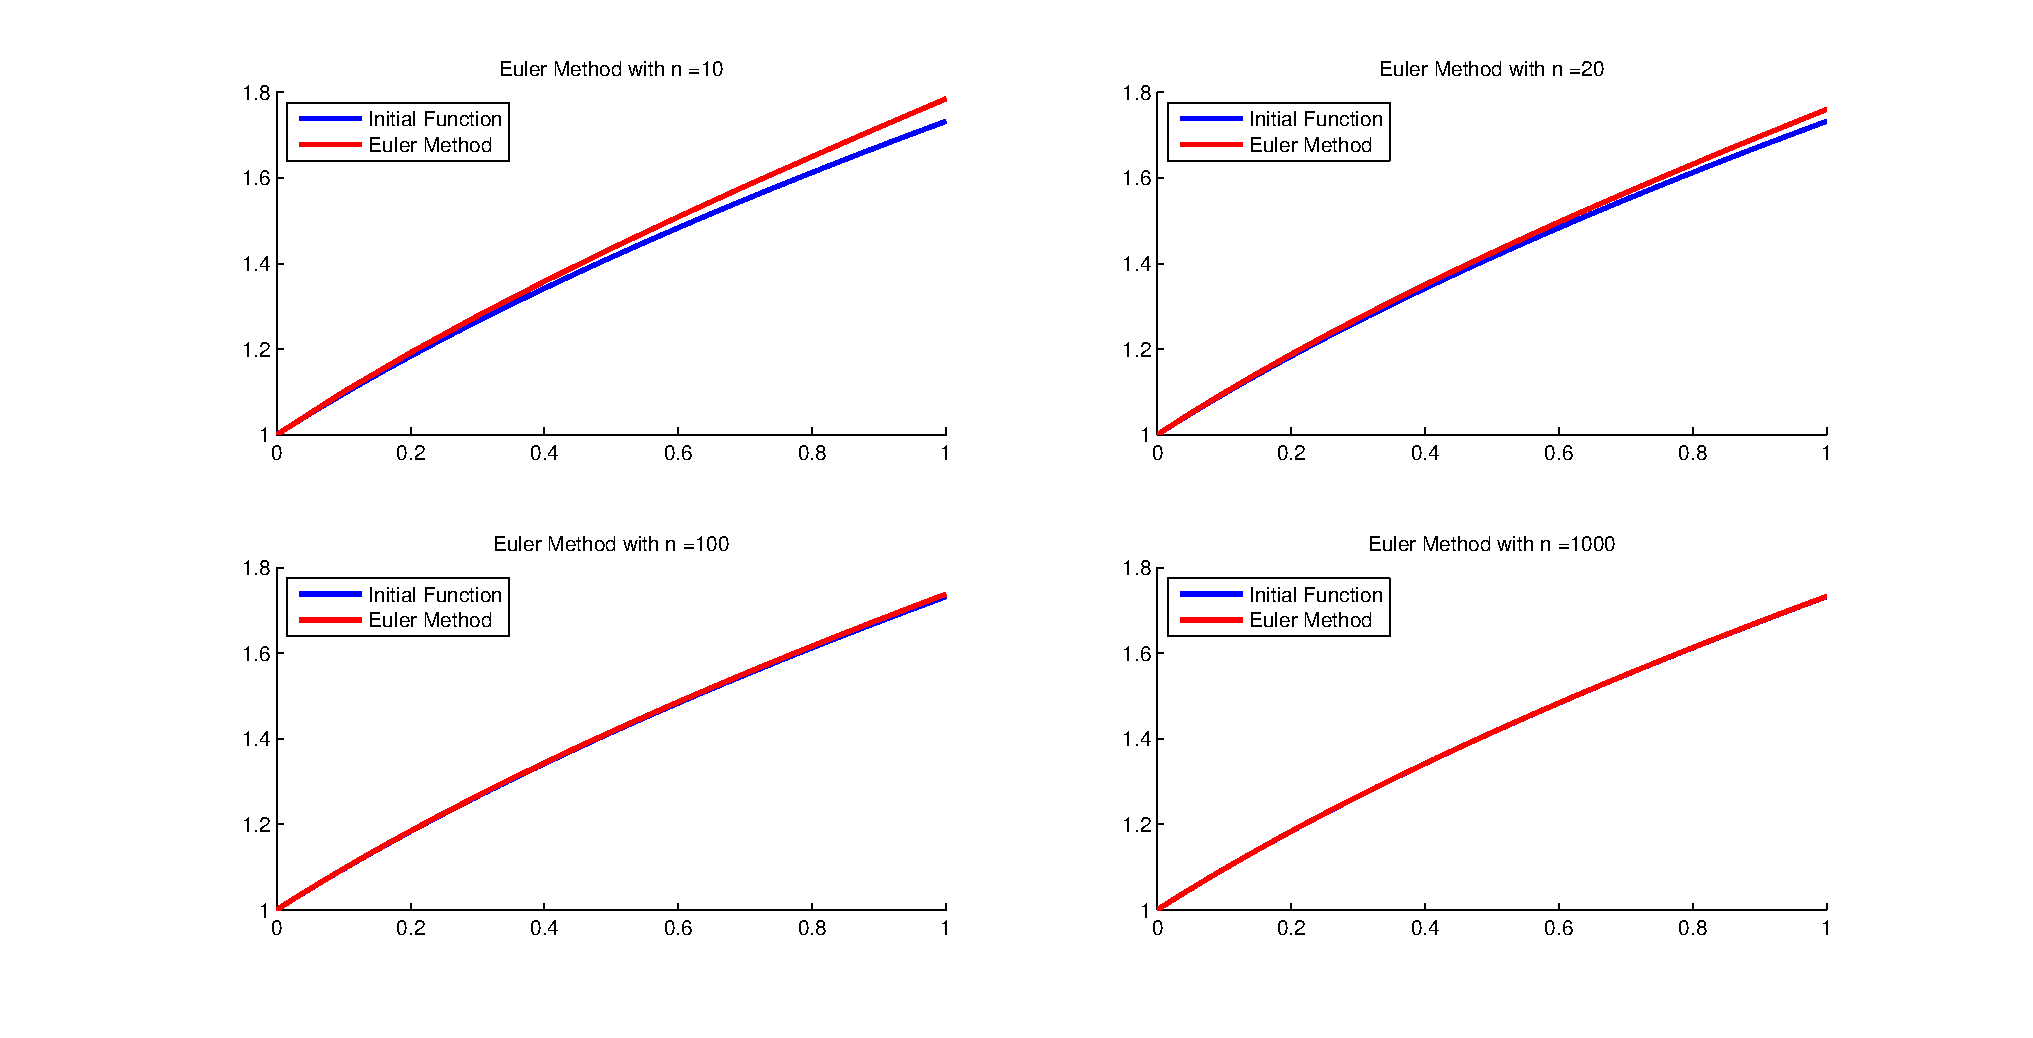
\includegraphics[width=1.0\textwidth]{../chapter5_1_1.eps}
						\caption{欧拉法与原始函数比较. 红色为欧拉法结果, 蓝色为原始函数. 左上为$n=10$, 右上为$n=20$, 左下为$n=100$, 右下为$n=1000$. 可以看到, 随着$n$增大, 红色曲线与蓝色曲线趋于重合}
						\label{img_chapter5_1_1}
					\end{figure}
						
						结果对比:\\
					\begin{tabular}{|c|c|c|c|c|}
						\hline
						$n$    & 10 & 20 & 100 & 1000\\
						\hline
						$y(1)$&1.78477083 & 1.76003786 & 1.73795017 & 1.73264816 \\
						\hline
						$Err$&-0.05272002 & -0.02798705 & -0.00589936 & -0.00059735 \\
						\hline
						$\max \left|y\left(1\right) - w_{n} \right|$ & 0.1288 & 0.0644 & 0.0129 & 0.0013\\
						\hline
					\end{tabular}
				\subparagraph{预估校正格式}
					Steps
					\begin{enumerate}
						\item 使用4阶Runge-Kutta方法, 估计出$y_1,y_2,y_3$的值.
						\item 使用4步Adams-Bashforth法作为预估:
						
						 $y_4^{\left(0\right)} = y_3 + \frac{h}{24}\left[55f\left(t_3,y_3\right) - 59f\left(t_2,y_2\right) + 37f\left(t_1,y_1\right) - 9f\left(t_0,y_0\right) \right]$
						\item 使用3步Adams-Moulton法作为校正:
						
						$y_{k+1} = y_i + \frac{h}{24}\left[9f\left(t_{i+1},y_{i+1}^{\left(k\right)}\right) + 19f\left(t_i,y_i\right) -5f\left(t_{i-1},y_{i-1}\right) + f\left(t_{i-2},y_{i-2}\right)\right]$
					\end{enumerate}
					代码:
					\begin{lstlisting}
					clear;
					left = 0; right = 1;
					f = @(x,y)y - 2*x/y; y0 = 1;
					n_lst = [10, 20, 100 ,1000];
					g = @(x)sqrt(2*x+1);
					X = left:(right - left)/50:right;Y = [];
					for i = 1:length(X)
						Y(i) = g(X(i));
					end
						
					for tp=1:length(n_lst)
						n = n_lst(tp); h = (right-left)/n;
						t = left; w = y0; A = [y0];
						for i=1:3
							K1 = h*f(t,w);
							K2 = h*f(t+h/2,w+K1/2);
							K3 = h*f(t+h/2,w+K2/2);
							K4 = h*f(t+h,w+K3);
							w = w + (K1 + 2*K2 +2*K3 + K4)/6;
							t = t + h; A(i+1) = w;
						end
						w3 = A(4); w2 = A(3); w1 = A(2); w0 = A(1);
						t3 = left + 3*h; t2 = left + 2*h; t1 = left + h; t0 = left;
						for i=4:n
							t = t + h;
							w = w3 + h*(55*f(t3,w3) - 59*f(t2,w2) +37*f(t1,w1)-9*f(t0,w0))/24;
							w = w3 + h*(9*f(t,w) + 19*f(t3,w3) - 5*f(t2,w2) + f(t1,w1))/24;
							t0 = t1; t1 = t2; t2 = t3; t3 = t;
							w0 = w1; w1 = w2; w2 = w3; w3 = w; A(i+1) = w;
						end
						fprintf('%d %.12f\n',n,A(n+1))
						subplot(2,2,tp);
						plot(X,Y,left:(right-left)/n:right,A);
						title(['Predictor-Corrector with n =' num2str(n)])
						legend('Initial Function','Predictor-Corrector',2)
					end
					\end{lstlisting}
					结果:\\
					\begin{tabular}{|c|c|c|c|c|}
						\hline
						$n$    & 10 & 20 & 100 & 1000\\
						\hline
						$f(1)$ &1.732050719875&1.732052801860&1.732050818170&1.732050807570\\
						\hline
						$Err$& 0.000000087694&-0.000001994291&-0.000000010601&-0.000000000001 \\
						\hline
					\end{tabular}
					\begin{figure}[H]
						\centering
						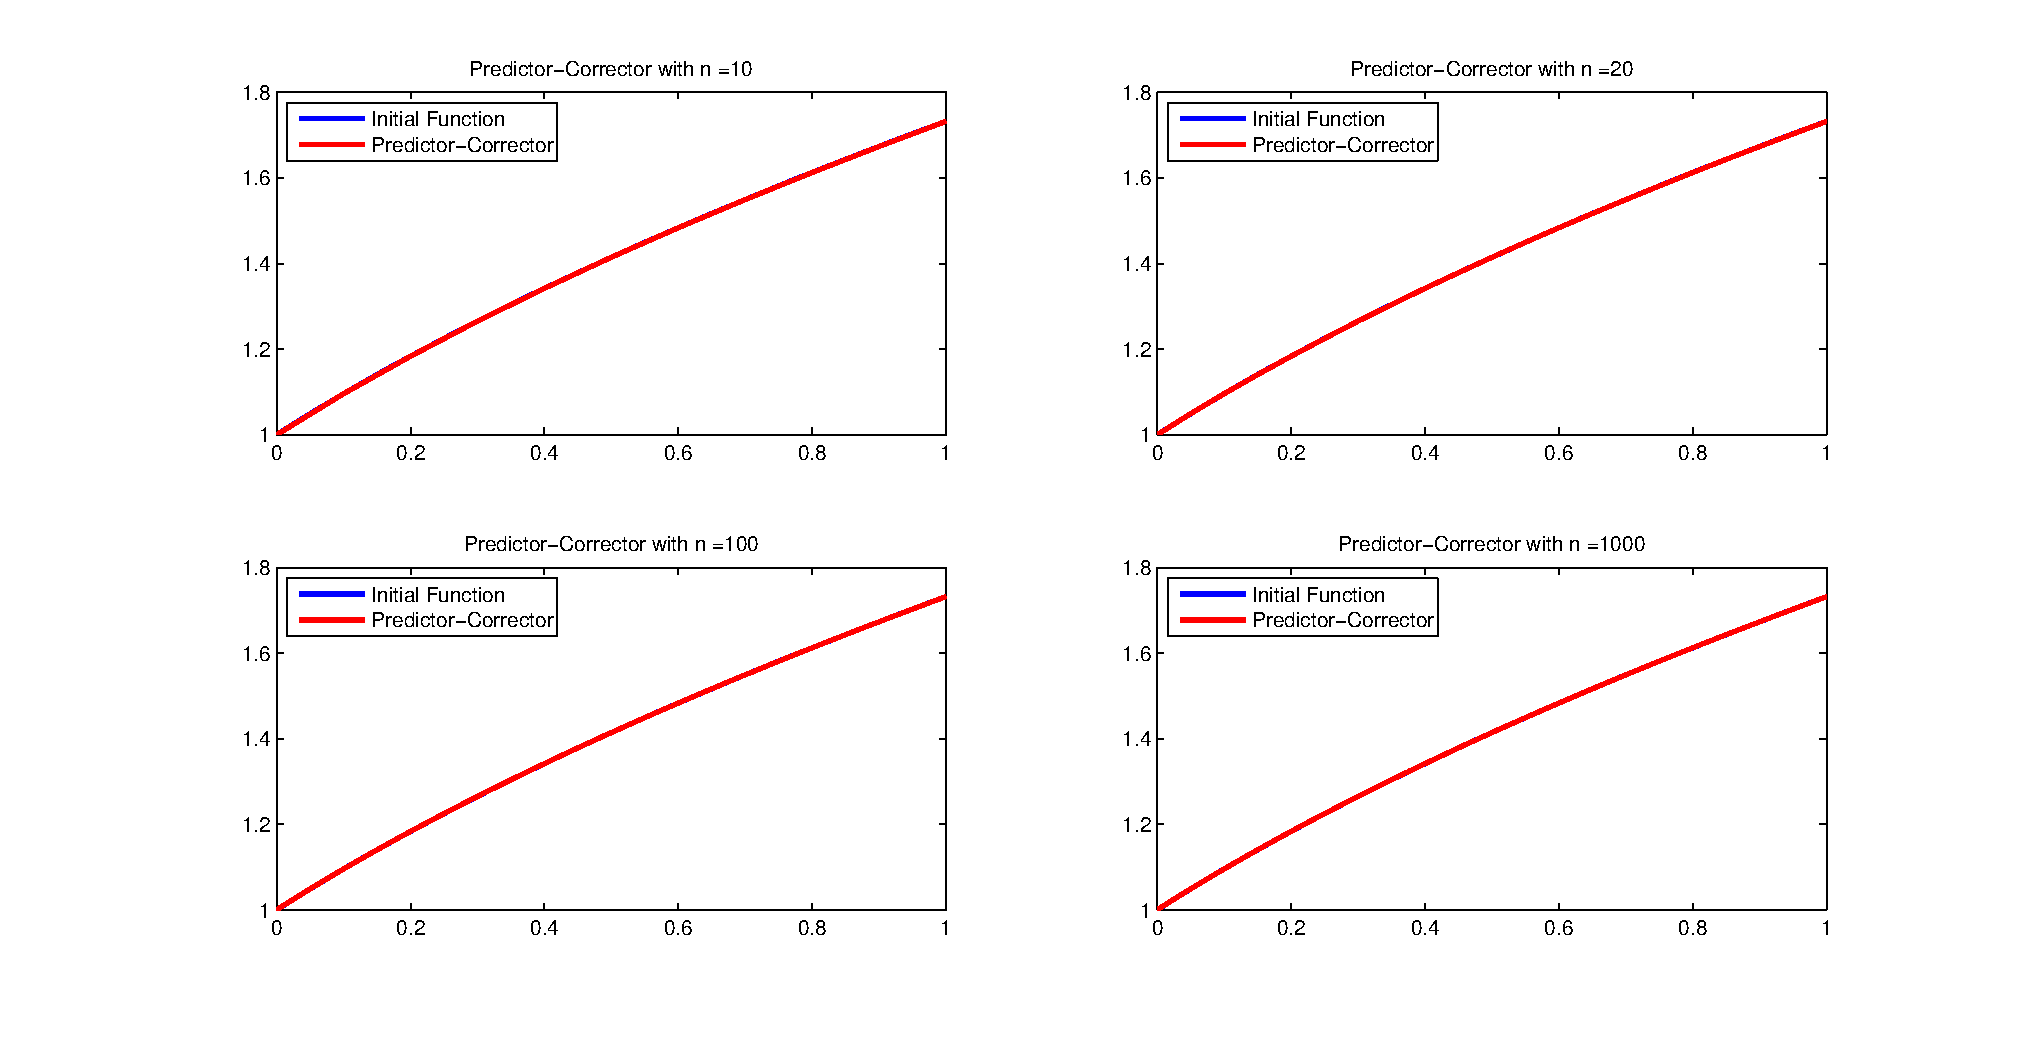
\includegraphics[width=1.0\textwidth]{../chapter5_1_2.eps}
						\caption{预估校正法与原始函数比较. 红色为预估校正法结果, 蓝色为原始函数. 左上为$n=10$, 右上为$n=20$, 左下为$n=100$, 右下为$n=1000$. 可以看出, 相比欧拉法而言, 预估校正法具有更高的精度. 对于$n=10$的情况, 两个函数曲线已经近似重合}
						\label{img_chapter5_1_2}
					\end{figure}
				\subparagraph{四阶龙格库塔格式}:
				
					代码:
					\begin{lstlisting}
						clear;
						left = 0; right = 1;
						f = @(x,y)y - 2*x/y; y0 = 1;
						n_lst = [10, 20, 100 ,1000];
						g = @(x)sqrt(2*x+1);
						X = left:(right - left)/50:right; Y = [];
						for i = 1:length(X)
							Y(i) = g(X(i));
						end
						for tp=1:length(n_lst)
							n = n_lst(tp); h = (right-left)/n;
							t = left; w = y0; A = [y0];
							for i=1:n
								K1 = h*f(t,w);
								K2 = h*f(t+h/2,w+K1/2);
								K3 = h*f(t+h/2,w+K2/2);
								K4 = h*f(t+h,w+K3);
								w = w + (K1 + 2*K2 +2*K3 + K4)/6;
								t = t + h;
								A(i+1) = w;
							end
							fprintf('%f\n',A(n+1))
							subplot(2,2,tp);
							plot(X,Y,left:(right-left)/n:right,A);
							title(['Runge-Kutta with n =' num2str(n)])
							legend('Initial Function','Runge-Kutta',2)
						end
					\end{lstlisting}
					结果:\\
					\begin{tabular}{|c|c|c|c|c|}
						\hline
						$n$    & 10 & 20 & 100 & 1000\\
						\hline
						$f(1)$ &1.732056365166 &1.732051148140 &1.732050808103 &1.732050807569\\
						\hline
						$Err$ &-0.000005557597&-0.000000340571&-0.000000000534&-0.000000000000 \\
						\hline
					\end{tabular}
					\begin{figure}[H]
						\centering
						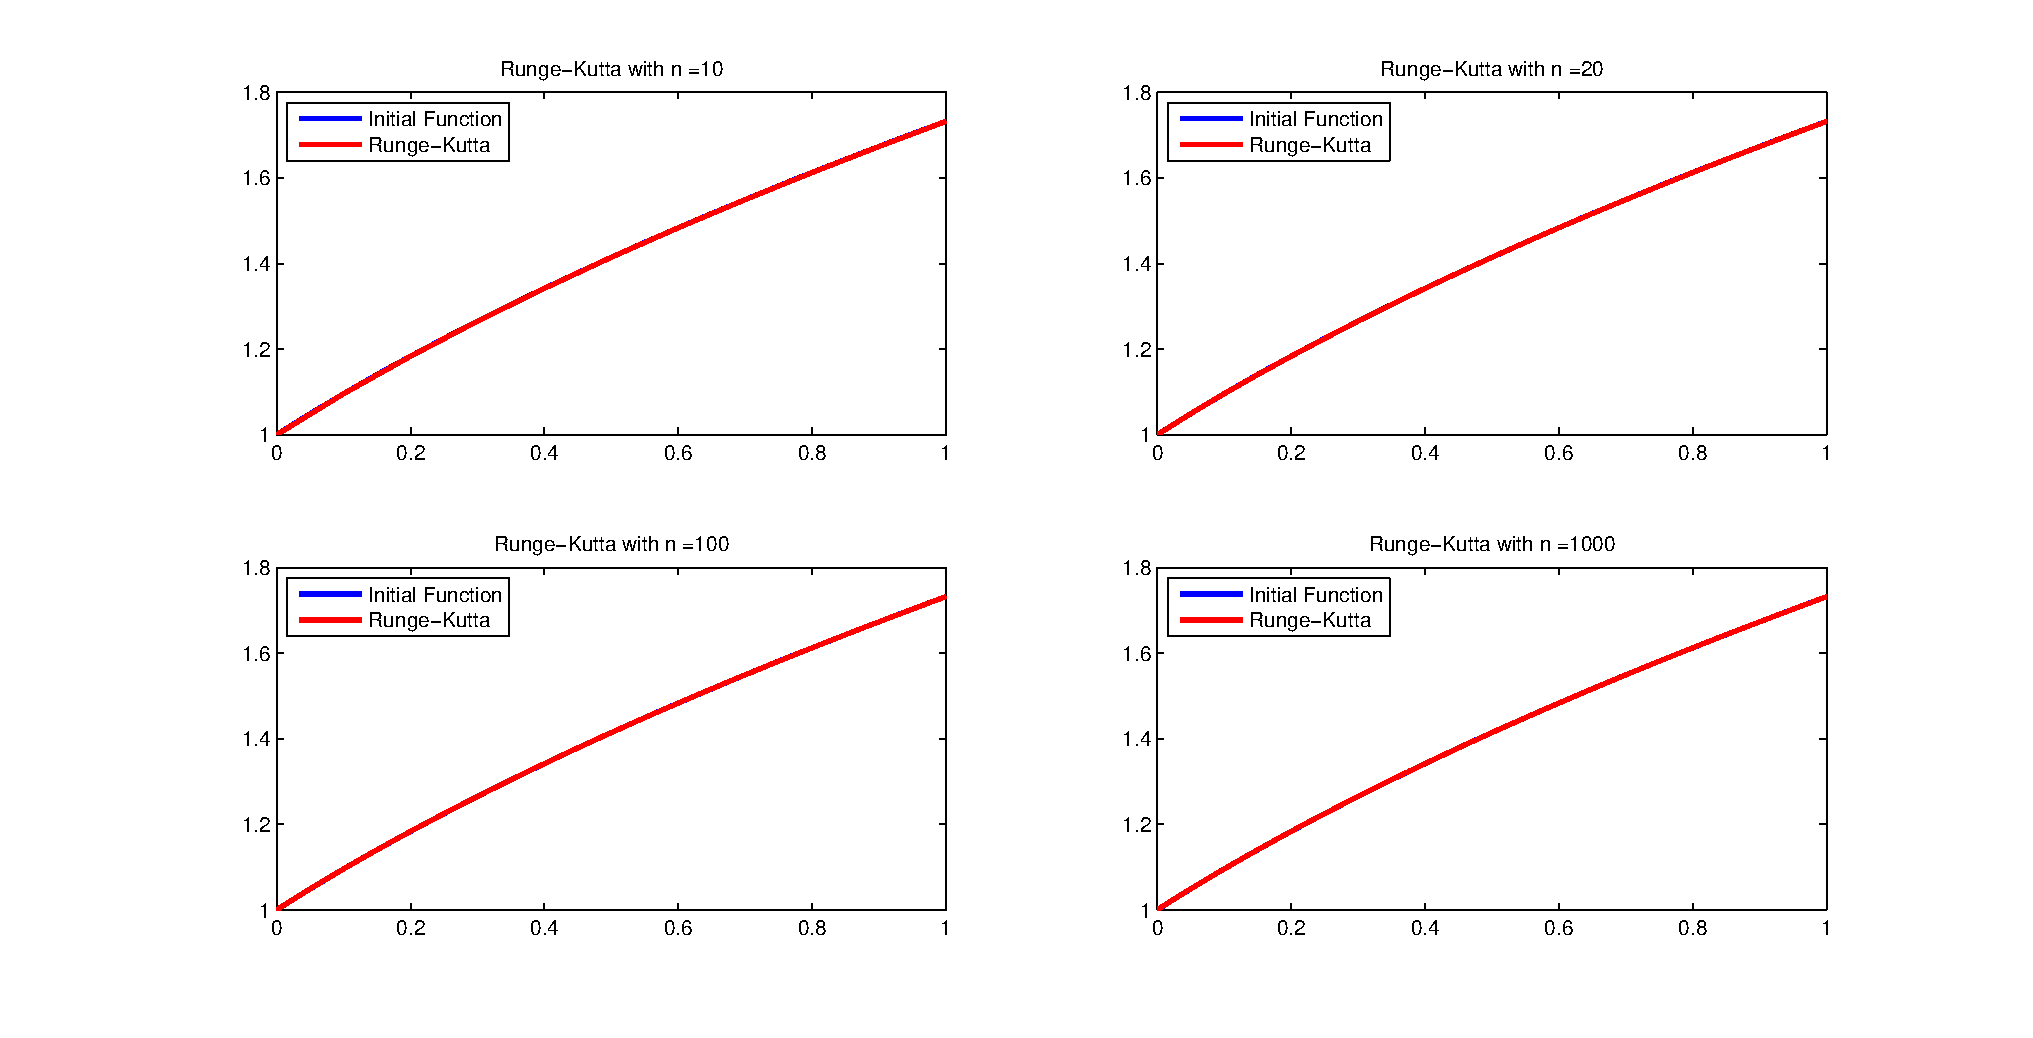
\includegraphics[width=1.0\textwidth]{../chapter5_1_3.eps}
						\caption{龙格-库塔与原始函数比较. 红色为龙格-库塔法结果, 蓝色为原始函数. 左上为$n=10$, 右上为$n=20$, 左下为$n=100$, 右下为$n=1000$. 可以看出, 在$n=10$的情况, 两个函数曲线已经近似重合}
						\label{img_chapter5_1_3}
					\end{figure}
		\subsection{Problem 2}
			\paragraph{题目描述}
			:\newline
			求解描述振荡器的经典的van der Pol微分方程
			$$\left\{
				\begin{aligned}
					& \frac{d^2 y}{dt^2} - \mu \left(1-y^2 \right) \frac{dy}{dt} + y = 0 \\
					& y\left(0\right) = 1, y'\left(0 \right) = 0
				\end{aligned}
			\right.$$
			试分别取$\mu = 10, 1, 0.1$, 分别用龙格库塔四阶格式计算其数值解, 并作图比较$\mu$的大小对解的影响.
			
			\paragraph{Analysis}
			
			\subparagraph{常微分方程组解法}
			给定一个常微分方程组:
			$$\left\{
				\begin{aligned}
					\frac{dy_1}{dx} &= f_1\left(x,y_1,y_2,\cdots,y_n \right) \\
					\frac{dy_2}{dx} &= f_2\left(x,y_1,y_2,\cdots,y_n \right) \\
					&\vdots \\
					\frac{dy_n}{dx} &= f_n\left(x,y_1,y_2,\cdots,y_n \right)
				\end{aligned}
			\right.$$
			
			初始状态$y_0^{\left(0\right)}, y_2^{\left(0\right)}, \cdots, y_n^{\left(0\right)}$已知.令$$
			\left\{
				\begin{aligned}
					K_{i}^{\left(1\right)} &= h * f_i\left(x^{\left(k\right)},y_1^{\left(k\right)},\cdots,y_n^{\left(k\right)}\right) \\
					K_{i}^{\left(2\right)} &= h * f_i\left(x^{\left(k\right)} + \frac{h}{2}, y_1^{\left(k\right)} + \frac{1}{2}K_{1}^{\left(1\right)}, \cdots, y_n^{\left(k\right)} + \frac{1}{2}K_{n}^{\left(1\right)}\right) \\
					K_{i}^{\left(3\right)} &= h * f_i\left(x^{\left(k\right)} + \frac{h}{2}, y_1^{\left(k\right)} + \frac{1}{2}K_{1}^{\left(2\right)}, \cdots, y_n^{\left(k\right)} + \frac{1}{2}K_{n}^{\left(2\right)}\right) \\
					K_{i}^{\left(4\right)} &= h * f_i\left(x^{\left(k\right)} + h, y_1^{\left(k\right)} + K_{1}^{\left(3\right)}, \cdots, y_n^{\left(k\right)} + K_{n}^{\left(3\right)}\right) \\										
				\end{aligned}
			\right.$$
			
			\subparagraph{高阶微分方程数值解}
				给定一个$n$阶微分方程, 且知道这个方程在某初始点处函数值和$1$到$n-1$阶导数值.求解方程:
				$$y^{\left(n\right)} = f\left(x,y,y^{'},\cdots,y^{\left(n-1 \right)} \right)$$
				令$y = y_1, y^{'} = y_2, y^{''} = y_3, \cdots, y^{\left(n-1\right)} = y_{n}$
				可以转化为下面的形式:
				$$\left\{
					\begin{aligned}
						y &= y_1 \\
						\frac{dy_1}{dx} &= y_2 \\
						\frac{dy_2}{dx} &= y_3 \\
						&\vdots \\ 
						\frac{dy_{n}}{dx} &= f\left(x,y,y_1,\cdots,y_{n}\right)
					\end{aligned}
				\right.$$
				于是这个问题转化为前面的$n$阶
			\subparagraph{本问题求解}
			令$$\left\{
				\begin{aligned}
					y_1 = y \\
					y_2 = y_1^{'}
				\end{aligned}
			 \right.$$
			 将Van der Pol微分方程化成标准形式:
			 $$\left\{
			 	\begin{aligned}
			 		y_1^{'} &= y_2 \\
			 		y_2^{'} &= \mu \left(1-y_1^2 \right)y_2 - y_1
			 	\end{aligned}
			 \right.$$
			 
			 代码:
			 
			 \begin{lstlisting}
			 	clear;
			 	left = 0; right = 30; y1_0 = 1; y2_0 = 0;
			 	n = 3000; h = (right-left)/n; miu_lst = [10, 1, 0.1];
			 	f1 = @(t,y1,y2)y2; P = [];
			 	for tp=1:length(miu_lst)
			 		miu = miu_lst(tp);
			 		f2 = @(t,y1,y2)miu*(1-y1*y1)*y2 - y1;
			 		y1 = y1_0; y2 = y2_0; A = [y1];
			 		for i=1:n
			 			t = left + i*h;
			 			K11 = h*f1(t, y1, y2);
			 			K21 = h*f2(t, y1, y2);
			 	
			 			K12 = h*f1(t + h/2, y1 + K11/2, y2 + K21/2);
					 	K22 = h*f2(t + h/2, y1 + K11/2, y2 + K21/2);
			 	
			 			K13 = h*f1(t + h/2, y1 + K12/2, y2 + K22/2);
					 	K23 = h*f2(t + h/2, y1 + K12/2, y2 + K22/2);
			 	
			 			K14 = h*f1(t + h, y1 + K13, y2 + K23);
					 	K24 = h*f2(t + h, y1 + K13, y2 + K23);
			 	
					 	y1 = y1 + (K11 + 2*K12 + 2*K13 + K14)/6;
					 	y2 = y2 + (K21 + 2*K22 + 2*K23 + K24)/6;
					 	A(i+1) = y1;
				 	end
				 	subplot(2,2,tp);
				 	plot(left:(right-left)/n:right,A);
				 	title(['with mu = ' num2str(miu)]);
				 	P = [P; A];
			 	end
			 	subplot(2,2,4); X = left:(right-left)/n:right;
			 	plot(X,P(1,:),X,P(2,:),X,P(3,:));
			 	title('All')
			 	legend(['with mu = ' num2str(miu_lst(1))],['with mu = ' num2str(miu_lst(2))],['with mu = ' num2str(miu_lst(3))])
			 \end{lstlisting}
			 \begin{figure}[H]
			 	\centering
			 	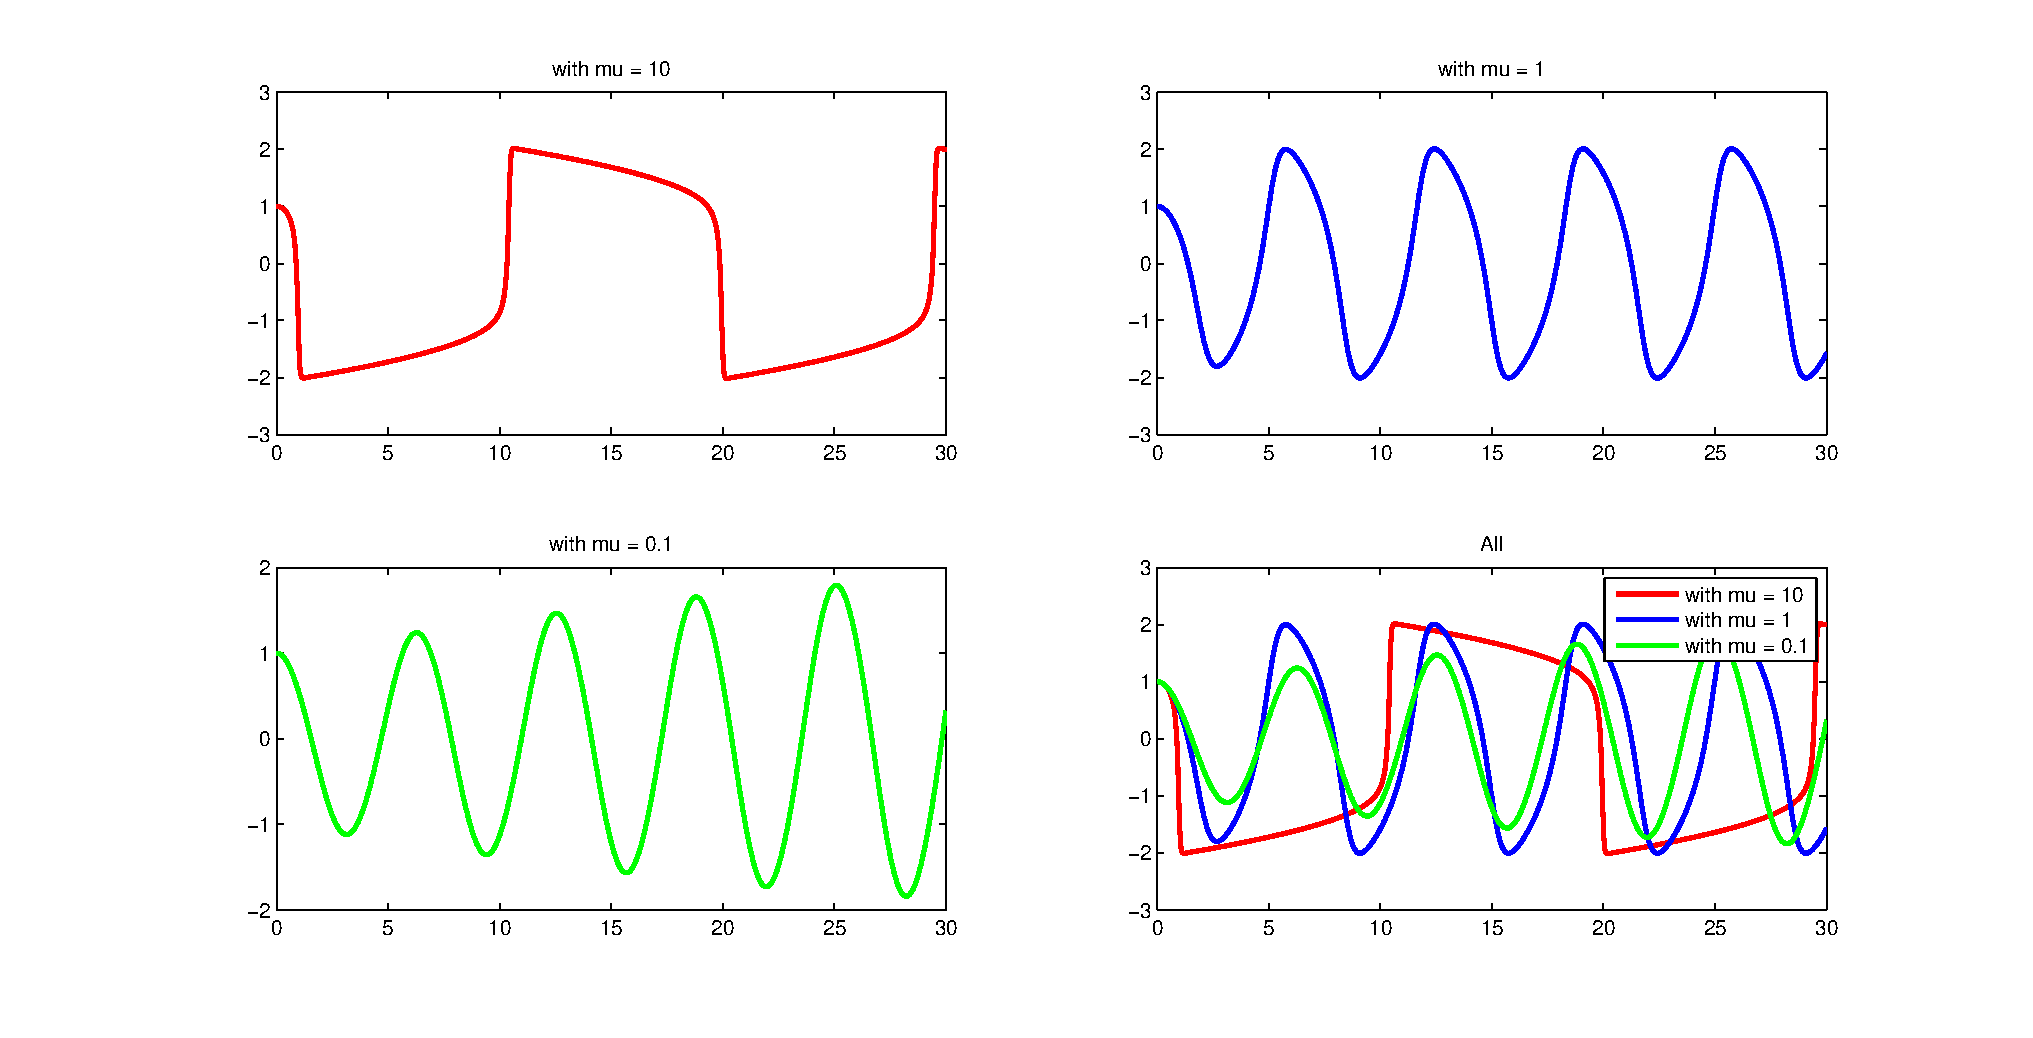
\includegraphics[width=1.0\textwidth]{../chapter5_2_1.eps}
			 	\caption{龙格-库塔求解高阶微分方程(Van der Pol方程). 左上为$\mu = 10$的情况, 右上为$\mu = 1$的情况,
			 	右下为$3$种情况对比}
			 	\label{img_chapter5_2_1}
			 \end{figure}
		 	结论: 当$\mu$减小时, 函数变得更加光滑, 且震荡速率加快.
	\section{Chapter 6}
		\subsection{Problem 1}
			\paragraph{题目描述}
			:\newline
				求矩阵
				$$ \mathbf{A} = 
					\left(
					\begin{matrix}
						2 & -1 & 1 \\
						3 &  3 & 9 \\
						3 &  3 & 5
					\end{matrix}
					\right)$$
				的LU分解.
			\paragraph{LU分解形式}
			:\newline
				设$\mathbf{A} = \left(a_{i,j}\right)_{n \times n}$, 分解为$\mathbf{A} = \mathbf{LU}$的形式, 其中$\mathbf{L}$为对角元为1的下三角矩阵, $\mathbf{U}$为上三角矩阵. 即
				$$
				\left(
					\begin{matrix}
						a_{11} & a_{12} & \cdots & a_{1n} \\
						a_{21} & a_{22} & \cdots & a_{2n} \\
						\vdots & \vdots & \ddots & \vdots \\
						a_{n1} & a_{n2} & \cdots & a_{nn} \\
					\end{matrix}
				\right) =
				\left(
					\begin{matrix}
						1 & 0 & \cdots & 0 \\
						l_{21} & 1 & \cdots & 0 \\
						\vdots & \vdots & \ddots & \vdots \\
						l_{n1} & l_{n2} & \cdots & 1 \\
					\end{matrix}
				\right) 
				\left(
				\begin{matrix}
					u_{11} & u_{12} & \cdots & u_{1n} \\
					0 & u_{22} & \cdots & u_{2n}\\
				\vdots & \vdots & \ddots & \vdots \\
				0 & 0 & \cdots & u_{nn} \\
				\end{matrix}
				\right)
				$$
				按照矩阵乘法规则, 比较系数, 可得
				$$
				\left\{
					\begin{aligned}
						u_{1j} &= a_{1j}  &\left(j=1,2,\cdots,n\right) \\
						l_{i1} &= \frac{a_{i1}}{u_{11}} &\left(i=2,3,\cdots,n \right)\\
						u_{ij} &= a_{ij} - \sum_{k=1}^{i-1}l_{ik}u_{kj} &\left(i=2,\cdots,n,j=i,\cdots,n\right) \\
						l_{ij} &= \left(a_{ij} - \sum_{k=1}^{j-1}l_{ik}u_{kj}\right) &\left(j=1,2,\cdots,n,i=j+1,\cdots,n\right)
					\end{aligned}
				\right.$$
			\paragraph{代码}
			:\newline
				\begin{lstlisting}
					clear;
					A  = [2,-1,1; 3,3,9; 3,3,5]
					n = length(A);
					L=eye(n,n); U=zeros(n,n);
					for k=1:n
						for j=k:n
							U(k,j)=A(k,j)-sum(L(k,1:k-1).*U(1:k-1,j)');
						end
						for i=k+1:n
							L(i,k)=(A(i,k)-sum(L(i,1:k-1).*U(1:k-1,k)'))/U(k,k);
						end
					end
					disp(L); disp(U);
				\end{lstlisting}
			\paragraph{结果}
				$\mathbf{L} = \left(\begin{matrix}
				 1.0000   &      0     &    0 \\
				1.5000  &  1.0000     &    0 \\
				1.5000  &  1.0000  &  1.0000 \\
				\end{matrix}\right)$
				$\mathbf{U} = \left(\begin{matrix}
				   2.0000  & -1.0000   & 1.0000 \\
				0   & 4.5000  &  7.5000 \\
				0    &     0  & -4.0000 \\
				\end{matrix}\right)$
				
				检验: $\mathbf{LU} = \mathbf{A}$.
		\subsection{Problem 2}
			\paragraph{题目描述}
			:\newline
				求一下对称矩阵的$LL^T$, $LDL^T$分解.
				$$ \mathbf{A} = 
				\left(
				\begin{matrix}
				2 & -1 & 0 \\
				-1 &  2 & -1 \\
				0 &  -1 & 2
				\end{matrix}
				\right)$$
			\paragraph{$LDL^T$分解}\
				对于正定对称矩阵$\mathbf{A}$, 可以分解为如下形式:
				$$\mathbf{A} = 
					\left(
						\begin{matrix}
							a_{11} & a_{12} & \cdots & a_{1n} \\
							a_{12} & a_{22} & \cdots & a_{2n} \\
							\vdots & \vdots & \ddots & \vdots \\
							a_{1n} & a_{2n} & \cdots & a_{nn} \\
						\end{matrix}
					\right) = \mathbf{LDL}^{T}$$
				$$ = \left(
				\begin{matrix}
					1 & 0 & \cdots & 0 \\
					l_{21} & 1 & \cdots & 0 \\
					\vdots & \vdots & \ddots & \vdots \\
					l_{n1} & l_{n2} & \cdots & 1 \\
				\end{matrix}
				\right)
				\left(
				\begin{matrix}
				d_{11} & 0 & \cdots & 0 \\
				0 & d_{22} & \cdots & 0 \\
				\vdots & \vdots & \ddots & \vdots \\
				0 & 0 & \cdots & d_{nn} \\
				\end{matrix}
				\right)
				\left(
				\begin{matrix}
				1 & l_{21} & \cdots & l_{n1} \\
				0 & 1 & \cdots & l_{n2} \\
				\vdots & \vdots & \ddots & \vdots \\
				0 & 0 & \cdots & 1 \\
				\end{matrix}
				\right)
				 $$
				 
				 $$ = 
				 \left(
				 \begin{matrix}
				 d_{11} & 0 & \cdots & 0 \\
				 l_{21}d_{11} & d_{22} & \cdots & 0 \\
				 \vdots & \vdots & \ddots & \vdots \\
				 l_{n1}d_{11} & l_{n2}d_{22} & \cdots & d_{nn} \\
				 \end{matrix}
				 \right)
				 \left(
				 \begin{matrix}
				 1 & l_{21} & \cdots & l_{n1} \\
				 0 & 1 & \cdots & l_{n2} \\
				 \vdots & \vdots & \ddots & \vdots \\
				 0 & 0 & \cdots & 1 \\
				 \end{matrix}
				 \right)
				 $$
				 
				 因此,
				 $$\left\{
				 	\begin{aligned}
				 		d_{11} &= a_{11} &\\ 
				 		l_{j1} &= \frac{a_{1j}}{d_{11}} &\left(j=2,\cdots,n\right)\\
				 		d_{ii} &= a_{ii} - \sum_{k=1}^{i-1}l_{ik}^2d_{kk} &\left( i=2,3,\cdots,n\right) \\
				 		l_{ji} &= \frac{a_{ij} - \sum_{k=1}^{i}l_{ik}l_{jk}d_{kk}}{d_{ii}} &\left(j=i+1,\cdots,n\right) \\
				 	\end{aligned}
				 \right. $$
			\paragraph{Code}:\newline
				\begin{lstlisting}
					clear;
					A = [2,-1,0;-1,2,-1;0,-1,2]; n = length(A);
					d = zeros(n,n); L = eye(n,n);
					d(1,1) = A(1,1);
					for j=2:n,L(j,1) = A(1,j)/d(1,1); end
					for i=2:n
						d(i,i) = A(i,i);
						for j=1:i-1
							d(i,i) = d(i,i) - L(i,j)^2 * d(j,j);
						end
						for j=i+1:n
							L(j,i) = A(i,j);
							for k=1:i-1
								L(j,i) = L(j,i) - L(i,k)*L(j,k)*d(k,k);
							end
							L(j,i) = L(j,i)/d(i,i);
						end
					end
					disp(L);disp(d)
				\end{lstlisting}
			\paragraph{Answer}
				$$\mathbf{L} = \left(
					\begin{matrix}
						1.0000    &     0      &   0 \\
						-0.5000  &  1.0000    &     0 \\
						0  & -0.6667   & 1.0000
					\end{matrix}
				\right)
				\mathbf{D} = \left(
					\begin{matrix}
						2.0000      &   0    &     0 \\
						0  &  1.5000     &    0 \\
						0   &      0 &   1.3333
					\end{matrix}
				\right)
				$$
				
				经检验, $\mathbf{LDL}^T = \mathbf{A}$.
			\paragraph{$\mathbf{LL}^T$分解} :\newline
				令$\mathbf{\overline{D}} = \left(\sqrt{d_{i,j}}\right)_{n \times n}$,
				 则$\mathbf{A} = \mathbf{LDL}^{T} = \mathbf{L\overline{D}\overline{D}L^T} = \left(\mathbf{L\overline{D}}\right)\left(\mathbf{L\overline{D}}\right)^T = \mathbf{\overline{L}}  \mathbf{\overline{L}}^T$.
				
			\paragraph{Code}:\newline
				\begin{lstlisting}
					clear;
					A = [2,-1,0;-1,2,-1;0,-1,2]; n = length(A);
					d = zeros(n,n); L = eye(n,n);
					d(1,1) = A(1,1);
					for j=2:n,L(j,1) = A(1,j)/d(1,1); end
					for i=2:n
						d(i,i) = A(i,i);
						for j=1:i-1
							d(i,i) = d(i,i) - L(i,j)^2 * d(j,j);
						end
						for j=i+1:n
							L(j,i) = A(i,j);
							for k=1:i-1
								L(j,i) = L(j,i) - L(i,k)*L(j,k)*d(k,k);
							end
							L(j,i) = L(j,i)/d(i,i);
						end
					end
					disp(L*sqrt(d))
				\end{lstlisting}
			\paragraph{Answer}
			
				$$\mathbf{\overline{L}} = \left(
					\begin{matrix}
						1.4142     &    0      &   0\\
						-0.7071 &   1.2247    &     0\\
						0  & -0.8165  &  1.1547
					\end{matrix}
				\right)$$
				经检验, $\mathbf{\overline{LL}}^T = A$.
	\section{Chapter 7}
		\subsection{Problem 1}
			\paragraph{题目描述}
			:\newline
				求解线性方程组
				$$\left\{
				\begin{aligned}
					4x_1 + 3x_2 &=24 \\
					3x_1 + 4x_2 &=30 \\
					-x_2 + 4x_3 &=-24
				\end{aligned}
				\right.$$
				分别利用Jacobi, Gauss-Seidel方法计算其数值解(取初始解向量$\mathbf{x}=\left(1,1,1\right)^T$), 对给定的收敛误差, 试比较不同范数($L_{\infty},L_2$)对迭代次数的影响.
			\paragraph{Jacobi}
				\subparagraph{Jacobi迭代法推导}
				假设方程组
				$$\left\{
					\begin{aligned}
						a_{11}x_1 &+ a_{12}x_2 + \cdots + a_{1n}x_n = b_1 \\ 
						a_{21}x_1 &+ a_{22}x_2 + \cdots + a_{2n}x_n = b_2 \\ 
						&\vdots \\
						a_{n1}x_1 &+ a_{n2}x_2 + \cdots + a_{nn}x_n = b_1 
					\end{aligned}
				\right.$$
				的系数矩阵$\mathbf{A}$非奇异, 不妨设$a_{ii} \neq 0\left(i=1,2,\cdots,n\right)$.将方程组变形为:
				$$\left\{
					\begin{aligned}
						x_1 = \frac{1}{a_{11}}&\left(-a_{12}x_2 -a_{13}x_3 -\cdots - a_{1n}x_n +b_1\right) \\
						x_2 = \frac{1}{a_{22}}&\left(-a_{21}x_1 -a_{23}x_3 -\cdots - a_{2n}x_n +b_2\right) \\
						&\vdots \\
						x_n = \frac{1}{a_{nn}}&\left(-a_{n1}x_1 -a_{n2}x_2 -\cdots - a_{n,n-1}x_{n-1} +b_n\right) 
					\end{aligned}
				\right.$$
				建立迭代公式:
				$$\left\{
					\begin{aligned}
						x_1^{\left(k+1\right)} = \frac{1}{a_{11}}&\left(-a_{12}x_2^{\left(k\right)} -a_{13}x_3^{\left(k\right)} -\cdots - a_{1n}x_n^{\left(k\right)} +b_1\right) \\
						x_2^{\left(k+1\right)} = \frac{1}{a_{22}}&\left(-a_{21}x_1^{\left(k\right)} -a_{23}x_3^{\left(k\right)} -\cdots - a_{2n}x_n^{\left(k\right)} +b_2\right) \\
						&\vdots \\
						x_n^{\left(k+1\right)} = \frac{1}{a_{nn}}&\left(-a_{n1}x_1^{\left(k\right)} -a_{n2}x_2^{\left(k\right)} -\cdots - a_{n,n-1}x_{n-1}^{\left(k\right)} +b_n\right) 
					\end{aligned}
				\right.$$
				选定初始向量$\mathbf{x}^{\left(0\right)}$后, 反复迭代可以得到向量序列$\left\{\mathbf{x}^{\left(k\right)} \right\}$
				迭代公式为:
				$$\left\{
					\begin{aligned}
						\mathbf{x}^{\left(0\right)} &= \left(x_1^{\left(0\right)},x_2^{\left(0\right),\cdots,x_n^{\left(0\right)}}\right)^T \\
						x_i^{\left(k+1\right)} &= \frac{1}{a_{ii}}\left(b_i - \sum_{j=1,j\neq i}^{n}a_{ij}x_j^{\left(k\right)} \right)
					\end{aligned}
				\right.$$
				
				Jacobi迭代法也可以写为向量递推的形式
				$$\mathbf{x}^{\left(k\right)} = \mathbf{T}\mathbf{x}^{\left(k\right)} + \mathbf{c}$$
				
				设$\mathbf{D}$是对角元与$\mathbf{A}$相同的对角阵; $-\mathbf{L}$是严格下三角矩阵, 下三角元素与$\mathbf{A}$相同; $-\mathbf{U}$是严格上三角矩阵, 上三角元素与$\mathbf{A}$相同. 因此$\mathbf{A} = \mathbf{D} - \mathbf{L} - \mathbf{U}$.
				
				对于方程$\mathbf{A} \mathbf{x} = \mathbf{b}$, 或$\left(\mathbf{D} - \mathbf{L} - \mathbf{U} \right) \mathbf{x} = \mathbf{b}$, 
				
				可以变形为$$\mathbf{D} \mathbf{x} = \left(\mathbf{L} + \mathbf{U} \right) \mathbf{x} + \mathbf{b}$$
				
				也就是$$\mathbf{x} = \mathbf{D}^{-1} \left(\mathbf{L} + \mathbf{U}\right) \mathbf{x} + \mathbf{D}^{-1}\mathbf{b}$$
				
				写成递推式的形式: $$\mathbf{x}^{\left(k\right)} = \mathbf{D}^{-1} \left(\mathbf{L} + \mathbf{U}\right) \mathbf{x}^{\left(k-1\right)} + \mathbf{D}^{-1}\mathbf{b}$$
				
				\subparagraph{问题分析}
				在本题中, 方程组系数矩阵
				$$\mathbf{A} = \left(
					\begin{matrix}
						4&3&0\\ 
						3&4&-1\\
						 0&-1&4
					\end{matrix}
				\right)$$
				由于$\left|\mathbf{A}\right| = 24 >0$, $\left|\mathbf{D} \right| > 0$, 且$\rho \left( \mathbf{T}\right) \approx 0.7906 < 1$, 因此迭代收敛.
				
				\subparagraph{Code}
				:\newline
					\begin{lstlisting}
						clear;
						A = [4,3,0; 3,4,-1; 0,-1,4];
						b = [24,30,-24];
						x0 = [1,1,1]; x = x0;
						TOL = 1e-6; N = 100;
						for k=1:N
							for i=1:length(x0)
								x(i) = b(i);
							for j=1:length(x0)
								if j == i,continue;end
									x(i) = x(i) - A(i,j)*x0(j);
								end
								x(i) = x(i)/A(i,i);
							end
							if norm(x-x0,Inf) < TOL
								fprintf('Answer = (%f,%f,%f), Iteration times: %d\n',x(1),x(2),x(3),k)
								return
							end
							x0 = x;
						end
						fprintf('No solution.\n')
					\end{lstlisting}
					对于2范数, 用如下方法求得:
					\begin{lstlisting}
						if norm(x-x0,2) < TOL
					\end{lstlisting}
				\subparagraph{Answer}
					$\mathbf{x} = \left(3.000000,4.000000,-5.000000\right)$, 与求解线性方程组结果一致.
					\begin{center}
						\begin{tabular}{|c|c|c|}
							\hline
							范数    & 2 & $\infty$ \\
							\hline
							迭代次数 & 69 & 68 \\
							\hline
						\end{tabular}
					\end{center}
					
				
					由于$\left|\left|\mathbf{x} \right|\right|_{\infty} \leq \left|\left|\mathbf{x} \right|\right|_2$,
					因此使用无穷范数收敛速度略快.
			\paragraph{Gauss-Seidel}
				\subparagraph{Gauss-Seidel迭代法推导} :
					如果把Jacobi迭代公式改成以下形式
					$$\left\{
						\begin{aligned}
							x_1^{\left(k+1\right)} = \frac{1}{a_{11}}&\left(-a_{12}x_2^{\left(k\right)} -a_{13}x_3^{\left(k\right)} -\cdots - a_{1n}x_n^{\left(k\right)} +b_1\right) \\
							x_2^{\left(k+1\right)} = \frac{1}{a_{22}}&\left(-a_{21}x_1^{\left(k+1\right)} -a_{23}x_3^{\left(k\right)} -\cdots - a_{2n}x_n^{\left(k\right)} +b_2\right) \\
							&\vdots \\
							x_n^{\left(k+1\right)} = \frac{1}{a_{nn}}&\left(-a_{n1}x_1^{\left(k+1\right)} -a_{n2}x_2^{\left(k+1\right)} -\cdots - a_{n,n-1}x_{n-1}^{\left(k+1\right)} +b_n\right) 
						\end{aligned}
					\right.$$
					选取初始向量$\mathbf{x}^{\left(0\right)}$, 用迭代公式:
					$$\left\{
						\begin{aligned}
							\mathbf{x}^{\left(0\right)} &= \left(x_1^{\left(0\right)},x_2^{\left(0\right),\cdots,x_n^{\left(0\right)}}\right)^T \\
							x_i^{\left(k+1\right)} &= \frac{1}{a_{ii}}\left(b_i - \sum_{j=1}^{i-1}a_{ij}x_j^{\left(k+1\right)} - \sum_{j=i+1}^{n}a_{ij}x_j^{\left(k\right)} \right)
						\end{aligned}
					\right.$$
					Gauss-Seidel迭代法也可以写为向量递推的形式:
					$$\mathbf{x}^{\left(k\right)} = \mathbf{T}_g\mathbf{x}^{\left(k\right)} + \mathbf{c}_g$$
					或
					$$\left(\mathbf{D} - \mathbf{L}\right) \mathbf{x}^{\left(k\right)} = \mathbf{U} \mathbf{x}^{\left(k-1 \right)} + \mathbf{b}$$
					即
					$$ \mathbf{x}^{\left(k\right)} = \left(\mathbf{D} - \mathbf{L}\right)^{-1}\mathbf{U}\mathbf{x}^{k-1} + \left(\mathbf{D} - \mathbf{L}\right)^{-1}\mathbf{b}$$
				\subparagraph{问题分析}:\newline
				在本题中, $\rho \left(\mathbf{T}_g \right) \approx 0.6250 < 1$, 因此迭代收敛.
				\subparagraph{code}
					\begin{lstlisting}
						clear;
						A = [4,3,0; 3,4,-1; 0,-1,4]; b = [24,30,-24];
						x = [1,1,1]; TOL = 1e-6; N = 100; x0 = x;
						for k=1:N
							for i=1:length(x)
								x(i) = b(i);
								for j=1:length(x)
									if j == i, continue; end
									x(i) = x(i) - A(i,j)*x(j);
								end
								x(i) = x(i)/A(i,i);
							end
							if norm(x-x0,Inf) < TOL
								fprintf('Answer = (%f,%f,%f), Iteration times: %d\n',x(1),x(2),x(3),k)
								return
							end
							x0 = x;
						end
						fprintf('No solution.\n')
					\end{lstlisting}
				\subparagraph{Answer}
					:\newline
					\begin{tabular}{|c|c|c|}
						\hline
						范数    & 2 & $\infty$ \\
						\hline
						迭代次数 & 27 & 27 \\
						\hline
						结果 & $\left(3.000001,3.999999,-5.000000\right)$ & $\left(3.000001,3.999999,-5.000000\right)$\\
						\hline
					\end{tabular}
				
					此时, 无穷范数迭代次数与$2$范数迭代次数相同.
					
					对比Jacobi迭代法, Gauss-Seidel迭代法收敛速度更快. 但是对于某些问题, 可能Jacobi法收敛速度更快, 甚至可能出现Gauss-Seidel不收敛的情况.
	\section{Chapter 8}
		\subsection{Problem 1}
			\paragraph{题目描述}
			:\newline
				[原书第八章习题一第13题(第9版本P509)]
				In a paper dealing with the efficiency of energy utilization of the larvae of the modest sphinx moth
				(Pachysphinx modesta), L. Schroeder [Schr1] used the following data to determine a relation between
				$W$, the live weight of the larvae in grams, and $R$, the oxygen consumption of the larvae in
				milliliters/hour. For biological reasons, it is assumed that a relationship in the form of $R$ = $bW^a$ exists
				between $W$ and $R$.
				\begin{enumerate}[(a)]
					\item Find the logarithmic linear least squares polynomial by using
					
					$\ln R = \ln b + a \ln W$.
					\item Compute the error associated with the approximation in part (a):
					$$ \sum\limits_{i=1}^{37}\left(R_i-bW_i^a \right)^2$$
					\item Modify the logarithmic least squares equation in part (a) by adding the quadratic term $c(\ln Wi)^2$,
					and determine the logarithmic quadratic least squares polynomial.
					\item Determine the formula for and compute the error associated with the approximation in part (c).
					
					\begin{tabular}{cc|cc|cc|cc|cc}
						\hline
						W & R &W &R& W& R& W& R& W& R \\
						\hline
						0.017 &0.154 &0.025 &0.23& 0.020 &0.181 &0.020& 0.180& 0.025 &0.234 \\
						0.087 &0.296 &0.111 &0.357 &0.085 &0.260 &0.119 &0.299 &0.233 &0.537 \\
						0.174 &0.363 &0.211 &0.366 &0.171 &0.334 &0.210 &0.428 &0.783 &1.47 \\
						1.11 &0.531 &0.999 &0.771 &1.29 &0.87 &1.32 &1.15 &1.35 &2.48 \\
						1.74 &2.23 &3.02 &2.01 &3.04 &3.59 &3.34 &2.83 &1.69 &1.44 \\
						4.09 &3.58 &4.28 &3.28 &4.29 &3.40 &5.48 &4.15 &2.75 &1.84 \\
						5.45 &3.52 &4.58 &2.96 &5.30 &3.88 &     &     &4.83 &4.66 \\
						5.96 &2.40 &4.68 &5.10 &     &     &     &     &5.53 &6.94 \\
						\hline
					\end{tabular}
				\end{enumerate} 
			\paragraph{Question 1}
				\subparagraph{推导}
					Cost Function: 
					$$Q = \sum_{i=1}^{m} \left(y_i -\beta_0 - \beta_1 x\right)^2$$
					为使Cost Function最小, 对$\beta_0,\beta_1$分别求偏导数,有
					$$\left\{
						\begin{aligned}
							\frac{\partial Q}{\partial \beta_0} &= -2\sum_{i=1}^{m}\left(y_i - \beta_0 - \beta_1 x_i \right) = 0 \\
							\frac{\partial Q}{\partial \beta_1} &= -2\sum_{i=1}^{m} \left(y_i - \beta_0 - \beta_1 x_i \right)x_i = 0
						\end{aligned}
					\right.$$
					求解方程组, 可得
					$$
						\left\{
							\begin{aligned}
								\beta_0 &= \frac{\sum\limits_{i=1}^{m} x_i^2 \sum\limits_{i=1}^{m}y_i - \sum\limits_{i=1}^{m}x_i y_i  \sum\limits_{i=1}^{m} x_i }{m\left(\sum\limits_{i=1}^{m}x_i^2 \right) - \left(\sum\limits_{i=1}^{m}x_i \right)^2}\\
								\beta_1 &= \frac{m\sum\limits_{i=1}^{m}x_i y_i - \sum\limits_{i=1}^{m}x_i \sum\limits_{i=1}^{m}y_i}{m\left(\sum\limits_{i=1}^{m}x_i^2 \right)^2 - \left(\sum\limits_{i=1}^{m}x_i \right)^2}	
							\end{aligned}
						\right.$$
				\subparagraph{Code}
					:\newline
					\begin{lstlisting}
						X = log(W); Y = log(R);
						A = mypoly(X,Y);
						left = min(X); right = max(X);
						f = @(a,b,x)a*x+b;
						DrX = [left-1/10*(right-left),right+1/10*(right-left)];
						DrY = [f(A(2),A(1),DrX(1)),f(A(2),A(1),DrX(2))];
						subplot(1,2,1);
						plot(X,Y,'*',DrX,DrY)
						legend('Initial Points','Linear Poly Fit',2);
						title('lnR = lnb + alnW');
						subplot(1,2,2)
						b = exp(A(1)); a = A(2);
						left = min(W); right = max(W);
						X1 = left:(right-left)/50:right; Y1 = W;
						for i=1:length(X1)
							Y1(i) = b*X1(i)^a;
						end
						plot(W,R,'*',X1,Y1);
						legend('Initial Points','Poly Fit',2);
						title('R = b*W^a')
						E = 0;
						for i=1:length(X)
							E = E + (R(i) - b*W(i)^a)^2;
						end
						disp(E)
					\end{lstlisting}
					求线性拟合最小二乘系数:
					\begin{lstlisting}
						function A = mypoly(x,y)
							sx = 0; sx2 = 0; n = length(x);
							sxy = 0; sy = 0;
							for i=1:n
								sx2 = sx2+x(i)*x(i);
								sy = sy + y(i);
								sx = sx + x(i);
								sxy = sxy + x(i)*y(i);
							end
							A = [0,0];
							A(1) = (sx2 * sy - sxy * sx)/(n*sx2 - sx*sx);
							A(2) = (n*sxy - sx*sy)/(n*sx2 - sx*sx);
						end
					\end{lstlisting}
				\subparagraph{Answer}
					\begin{figure}[H]
						\centering
						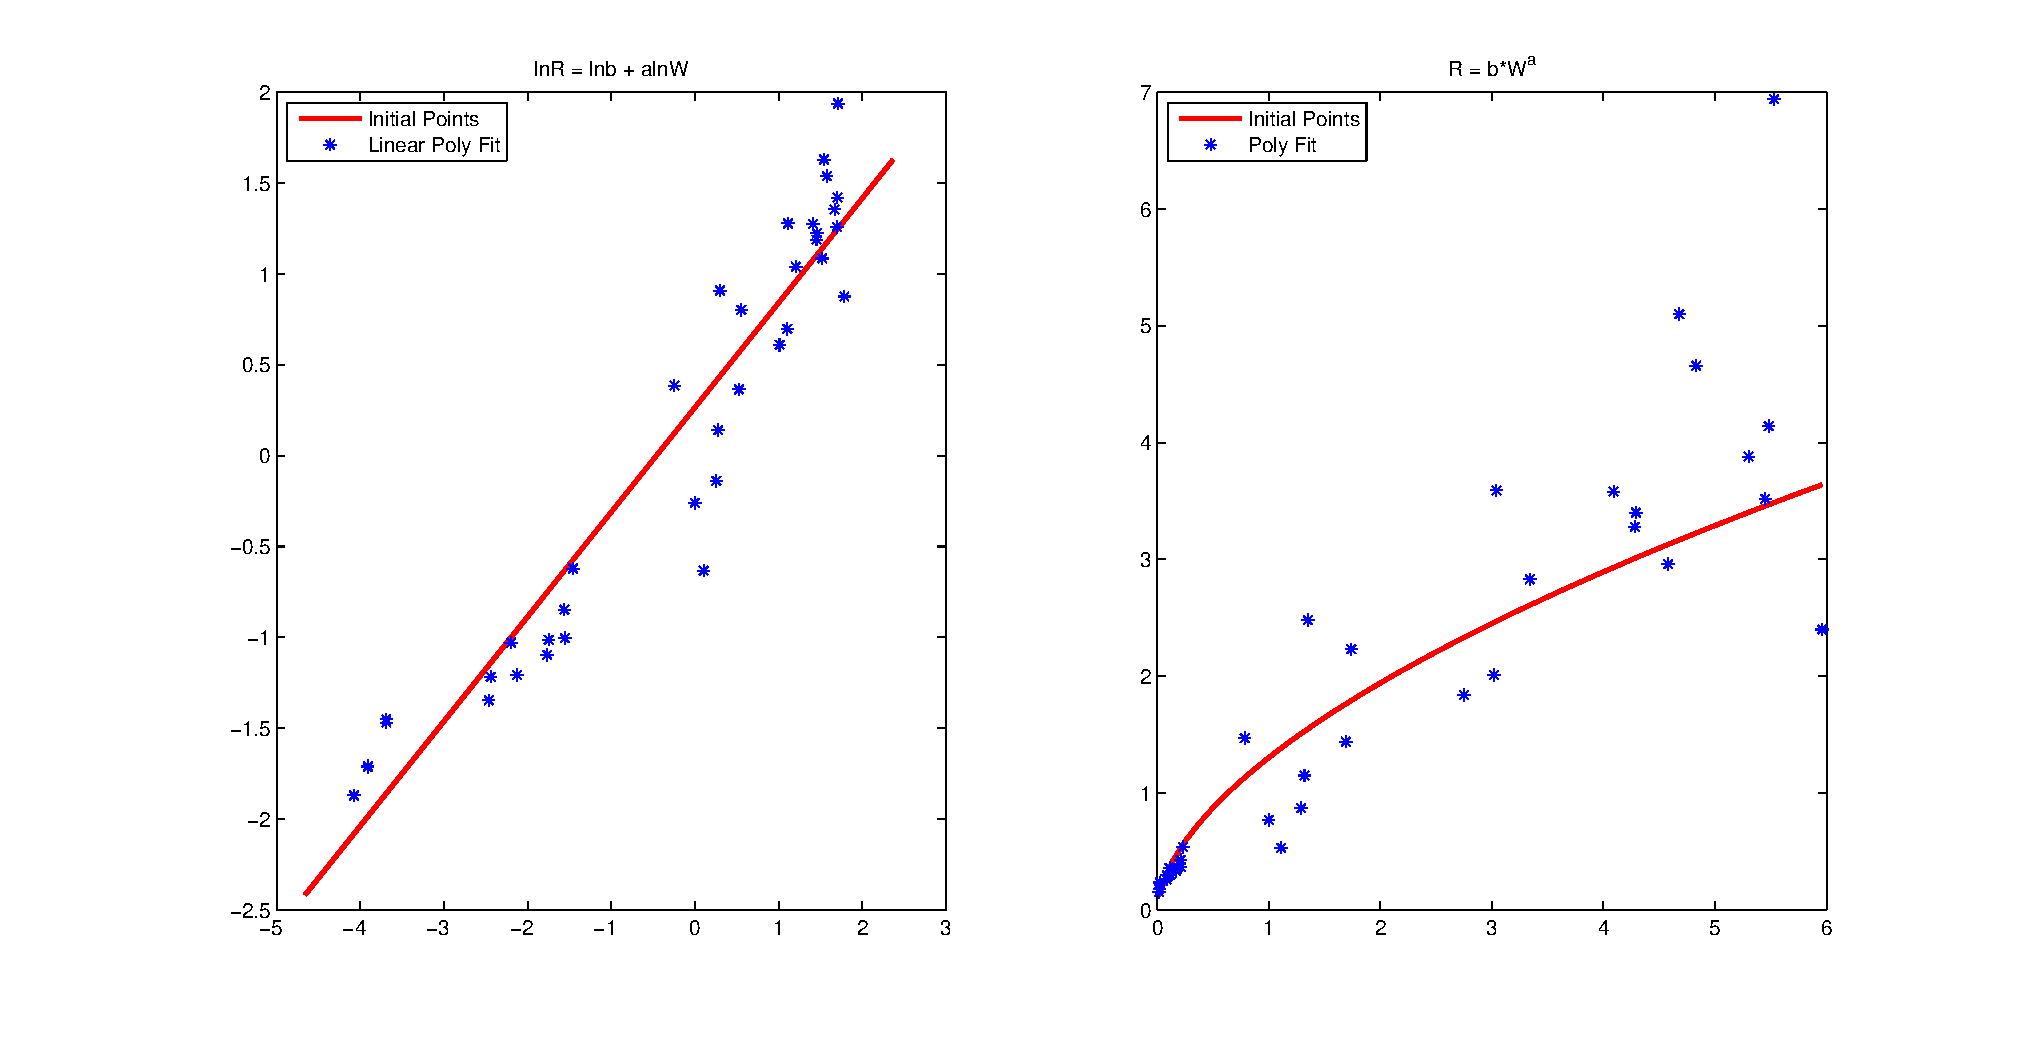
\includegraphics[width=1.0\textwidth]{../chapter_8_1.eps}
						\caption{拟合与原始点比较. 左图为$\ln R = \ln b + a \ln W$, 右图为$R = bW^a$}
						\label{img_chapter8_1}
					\end{figure}
					对于$\ln R = \ln b + a\ln W$,
					取$\ln b = 0.2646, a = 0.5756$   
				
			\paragraph{Question 2}:\newline
				对于误差公式$E = \sum\limits_{i=1}^{37}\left( R_i - bW_i^a\right)^2$, 计算可得$E = 25.2953$
			\paragraph{Question 3}
				\subparagraph{一般最小二乘多项式拟合形式}
				:\newline
					对于$P_n\left(x\right) = a_n x^n + a_{n-1} x^{n-1} + \cdots + a_1 x + a_0$
					目标:
					$$\min E = \sum\limits_{i=1}^{m} \left(y_i - P_n\left(x_i \right)\right)^2 = \sum\limits_{i=1}^{m}\left(y_i - \sum\limits_{k=1}^{n} a_k x_i^k\right)^2 $$
					令
					$$0 = \frac{\partial E}{\partial a_j} = -2\sum\limits_{i=1}^{m}y_i x_i^j + 2\sum\limits_{k=1}^{n}a_k \sum\limits_{i=1}x_i^{j+k} $$
					即
					$$ \sum\limits_{k=1}^{n}a_k \sum\limits_{i=1}x_i^{j+k} =\sum\limits_{i=1}^{m}y_i x_i^j $$
					令
					$$\mathbf{R} = \left(\begin{matrix}
						x_1^n  & x_1^{n-1} & \cdots & x_1 & 1 \\
						x_2^n  & x_2^{n-1} & \cdots & x_2 & 1 \\
						\vdots & \vdots    & \ddots & \vdots & \vdots \\
						x_m^n  & x_m^{n-1} & \cdots & x_m & 1
					\end{matrix} \right),
					\mathbf{a} = \left(\begin{matrix}
						a_n \\
						a_{n-1} \\
						\vdots \\
						a_{1} \\
						a_{0} 
					\end{matrix}\right),
					\mathbf{y} = \left(\begin{matrix}
						y_1 \\
						y_{2} \\
						\vdots \\
						y_{m-1} \\
						y_m
					\end{matrix}\right)
					$$
					则$\mathbf{R}^T \mathbf{Ra} = \mathbf{R}^T \mathbf{y}$, 即$\mathbf{a} = \left(\mathbf{R}^T \mathbf{R}\right)^{-1} \mathbf{R}^T \mathbf{y}$
				\subparagraph{Code}
					:\newline
					问题求解:
					\begin{lstlisting}
					X = log(W); Y = log(R);
					A = mypolyn(X,Y,2);
					disp(A)
					X_MIN = min(X); X_MAX = max(X); stp = X_MAX - X_MIN;
					X1 = X_MIN-0.1*stp:1.2*stp/100: X_MAX+0.1*stp; Y1 = X1;
					f = @(a,b,c,x)a*x*x+b*x+c;
					for i=1:length(X1)
						Y1(i) = f(A(3),A(2),A(1),X1(i));
					end
					subplot(1,2,1);
					plot(X,Y,'*',X1,Y1);
					legend('Initial Value','Poly Fit');
					title('lnR = a*(lnW)^2 + b*lnW + c');
					subplot(1,2,2);
					X1 = exp(X1); Y1 = exp(Y1);
					plot(W,R,'*',X1,Y1);
					legend('Initial Value','Fit Function');
					title('R = exp(a*(lnW)^2 + b*lnW + c)');
					E = 0;
					for i=1:length(W)
						E = E + (R(i) - exp(f(A(3),A(2),A(1),X(i))))^2;
					end
					disp(E)
					\end{lstlisting}
					多项式拟合
					\begin{lstlisting}
						function A = mypolyn(x,y,n)
							m = length(x); R = ones(m,n+1);
							for i=1:m
								for j=n:-1:1
									R(i,j) = R(i,j+1) * x(i,1);
								end
							end
							A = myLUsolver(R'*R, R'*y);
						end
					\end{lstlisting}
					LU分解求线性方程组的解:
					\begin{lstlisting}
				function MX = myLUsolver(A,b)
					n = length(A);
					L=eye(n,n); U=zeros(n,n);
					for k=1:n
						for j=k:n
							U(k,j)=A(k,j)-sum(L(k,1:k-1).*U(1:k-1,j)');
						end
						for i=k+1:n
							L(i,k)=(A(i,k)-sum(L(i,1:k-1).*U(1:k-1,k)'))/U(k,k);
						end
					end
					X=zeros(1,3);Y=zeros(1,3);
					Y(1)=b(1);
					for i=2:n    
						for j=1:i-1
							b(i)=b(i)-L(i,j)*Y(j);
						end
						Y(i)=b(i);
					end
					X(n)=Y(n)/U(n,n);
					for i=(n-1):-1:1
						for j=n:-1:i+1
							Y(i)=Y(i)-U(i,j)*X(j);
						end
						X(i)=Y(i)/U(i,i);
					end
					MX = X';
				end
					\end{lstlisting}
				\subparagraph{Answer}
					对于二次多项式拟合, 结果为:
					$\mathbf{a} = \left(0.0669 , 0.7006 ,0.0496\right)^T$.
					\begin{figure}[H]
						\centering
						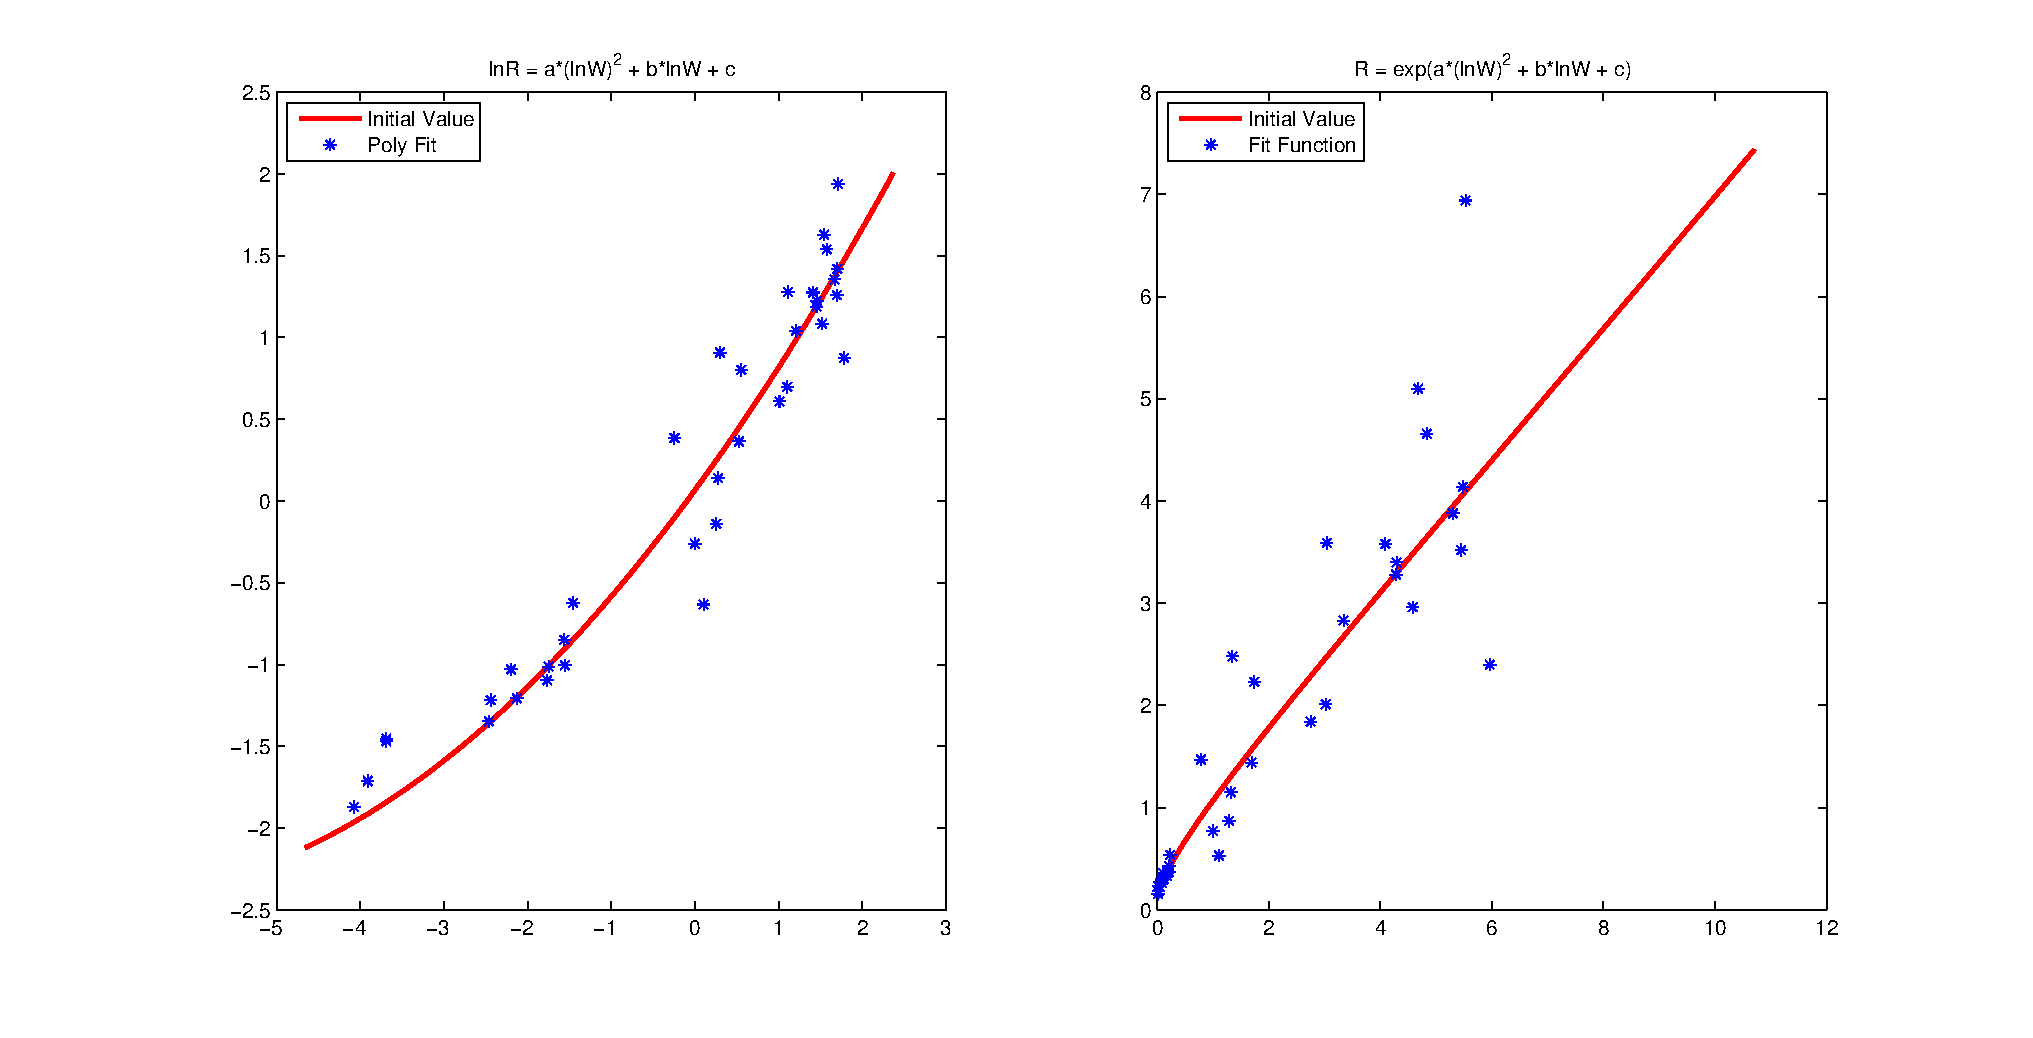
\includegraphics[width=1.0\textwidth]{../chapter_8_2.eps}
						\caption{拟合与原始点比较. 左图为$\ln R = a \left(\ln W\right)^2 + b \ln W + c$, 右图为$R = \exp \left(a \left(\ln W\right)^2 + b \ln W + c \right)$}
						\label{img_chapter8_2}
					\end{figure}
			\paragraph{Question 4}
			 $E=20.5971$
	\section{Chapter 9}
		\subsection{Problem 1}
			\paragraph{题目描述}:
				已知矩阵
				$$ \mathbf{A} = 
					\left(
						\begin{matrix}
							4 & -1 & 1 \\
							-1 &  3 & -2 \\
							1 &  -2 & 3
						\end{matrix}
					\right)$$
				是一个对称矩阵, 且其特征值为$\lambda_1=6,\lambda_2=3,\lambda_3=1$.分别利用幂法则, 对称幂法, 反幂法求其最大特征值和特征向量.
			
				注意: 可取初始向量$x^{\left(0\right)} = \left(1,1,1\right)^T$%
			
			\paragraph{幂法}
				\subparagraph{推导}
					假定$n\times n$的矩阵$\mathbf{A}$有$n$个特征值$\left|\lambda_1\right|> \left|\lambda_2\right| \geq \cdots \geq \left|\lambda_n\right|$, 对应线性无关的特征向量$\left\{\mathbf{v}^{\left(1\right)}, \mathbf{v}^{\left(2\right)},\cdots,\mathbf{v}^{\left(n\right)} \right\}$,
					
					$\forall \mathbf{x} \in \mathbb{R}^n, \exists \beta_1,\beta_2,\cdots,\beta_n, st \ \mathbf{x} = \beta_1 \mathbf{v}^{\left(1\right)} + \beta_2 \mathbf{v}^{\left(2\right)} + \cdots + \beta_n \mathbf{v}^{\left(n\right)} = \sum_{j=1}^{n} \beta_j \mathbf{v}^{\left(j\right)}$
					
					即
					$$
					\begin{aligned}
						\mathbf{Ax} = &\sum_{j=1}^{n} \beta_j \mathbf{Av}^{\left(j\right)} = \sum_{j=1}^{n} \beta_j \lambda_j \mathbf{v}^{\left(j\right)} \\
						\mathbf{A}^2\mathbf{x} = &\sum_{j=1}^{n} \beta_j \mathbf{Av}^{\left(j\right)} = \sum_{j=1}^{n} \beta_j \lambda_j^2 \mathbf{v}^{\left(j\right)} \\
						\mathbf{A}^2\mathbf{x} = &\sum_{j=1}^{n} \beta_j \mathbf{Av}^{\left(j\right)} = \sum_{j=1}^{n} \beta_j \lambda_j^2 \mathbf{v}^{\left(j\right)} \\
						&\vdots \\
						\mathbf{A}^k\mathbf{x} =& \sum_{j=1}^{n} \beta_j \mathbf{Av}^{\left(j\right)} = \sum_{j=1}^{n} \beta_j \lambda_j^k \mathbf{v}^{\left(j\right)} \\
						= &\lambda_1^k\left(\beta_1 \mathbf{v}^{\left(1\right)} + \sum_{j=2}^{n}\beta_j\left(\frac{\lambda_j}{\lambda_1}\right)^k\mathbf{v}^{\left(j\right)}\right)
					\end{aligned}$$
					由于
					$\forall j \in \left\{2,\cdots,n\right\}, \left|\lambda_1\right| > \left|\lambda_j\right|$
					,因此$\lim\limits_{k \to \infty}  \left(\frac{\lambda_j}{\lambda_1}\right)^k= 0$. 即
					$$\lim\limits_{k \to \infty} \mathbf{A}^k \mathbf{x} = \lim\limits_{k \to \infty}\lambda_1^k \beta_1 \mathbf{v}^{\left(1\right)}$$
					用$x_i^{\left(k\right)}$ 表示$\mathbf{x}^{\left(k\right)}$的第$i$个分量.由于
					$$\frac{x_i^{\left(k+1\right)}}{x_i^{\left(k\right)}} \approx \frac{\lambda_1^{k+1} \beta_1 \mathbf{v}_i^{\left(1\right)}}{\lambda_1^k \beta_1 \mathbf{v}_i^{\left(k\right)}} = \lambda_1$$
					需要注意, 当$\left|\lambda_1 \right| > 1$时, $\mathbf{x}^{\left(k\right)}$的各分量趋于无穷, 当$\left|\lambda_1\right| < 1$时, $\mathbf{x}^{\left(k\right)}$的各分量趋于0. 为了克服这一缺点, 需要将迭代向量规范化. 采用如下方式进行迭代:
					$$
					\left\{
						\begin{aligned}
							\mathbf{x}^{\left(0\right)} &= \mathbf{y}^{\left(0\right)} \neq \mathbf{0} \\
							\mathbf{x}^{\left(k\right)} &= \mathbf{Ay}^{\left(k-1\right)} \\
							\mathbf{y}^{\left(k\right)} & = \frac{\mathbf{x}^{\left(k\right)}}{\left|  \left|\mathbf{x}^{\left(k\right)} \right|\right|_{\infty}}
						\end{aligned}
					\right.$$
					
					$$\lim\limits_{k \to \infty} \mathbf{y}^{\left(k\right)} = \frac{v^{\left(1\right)}}{\left|\left|\mathbf{v}^{\left(1\right)} \right| \right|}, \lim\limits_{k \to \infty} \left|\left|\mathbf{x} \right| \right|_{\infty } = \lambda_1$$.
					
					易知最终的$\mathbf{x}$为所求特征向量.
				\subparagraph{Code} :\newline
					\begin{lstlisting}
						clear;
						A = [4,-1,1;-1,3,-2;1,-2,3]; n = length(A);
						x0 = [1;1;1]; y0 = x0; N = 100; TOL = 1e-7;
						mx0 = max(x0);
						for i=1:N
							x = A*y0; mx = max(x);
							y0 = x/mx;
							if abs(mx-mx0) < TOL
								fprintf('Answer %f Iteration time %d\n',mx,i)
								disp(x);
								return
							end
							x0 = x; mx0 = mx;
						end
						fprintf('No Solution\n');
					\end{lstlisting}
				\subparagraph{Answer}
					Max Eigen Value: 6.000000, Iteration time 27.\\
					Eigen Vector: $\mathbf{x} = \left(6.0000,-6.0000,6.0000 \right)^T$
					\begin{figure}[H]
						\centering
						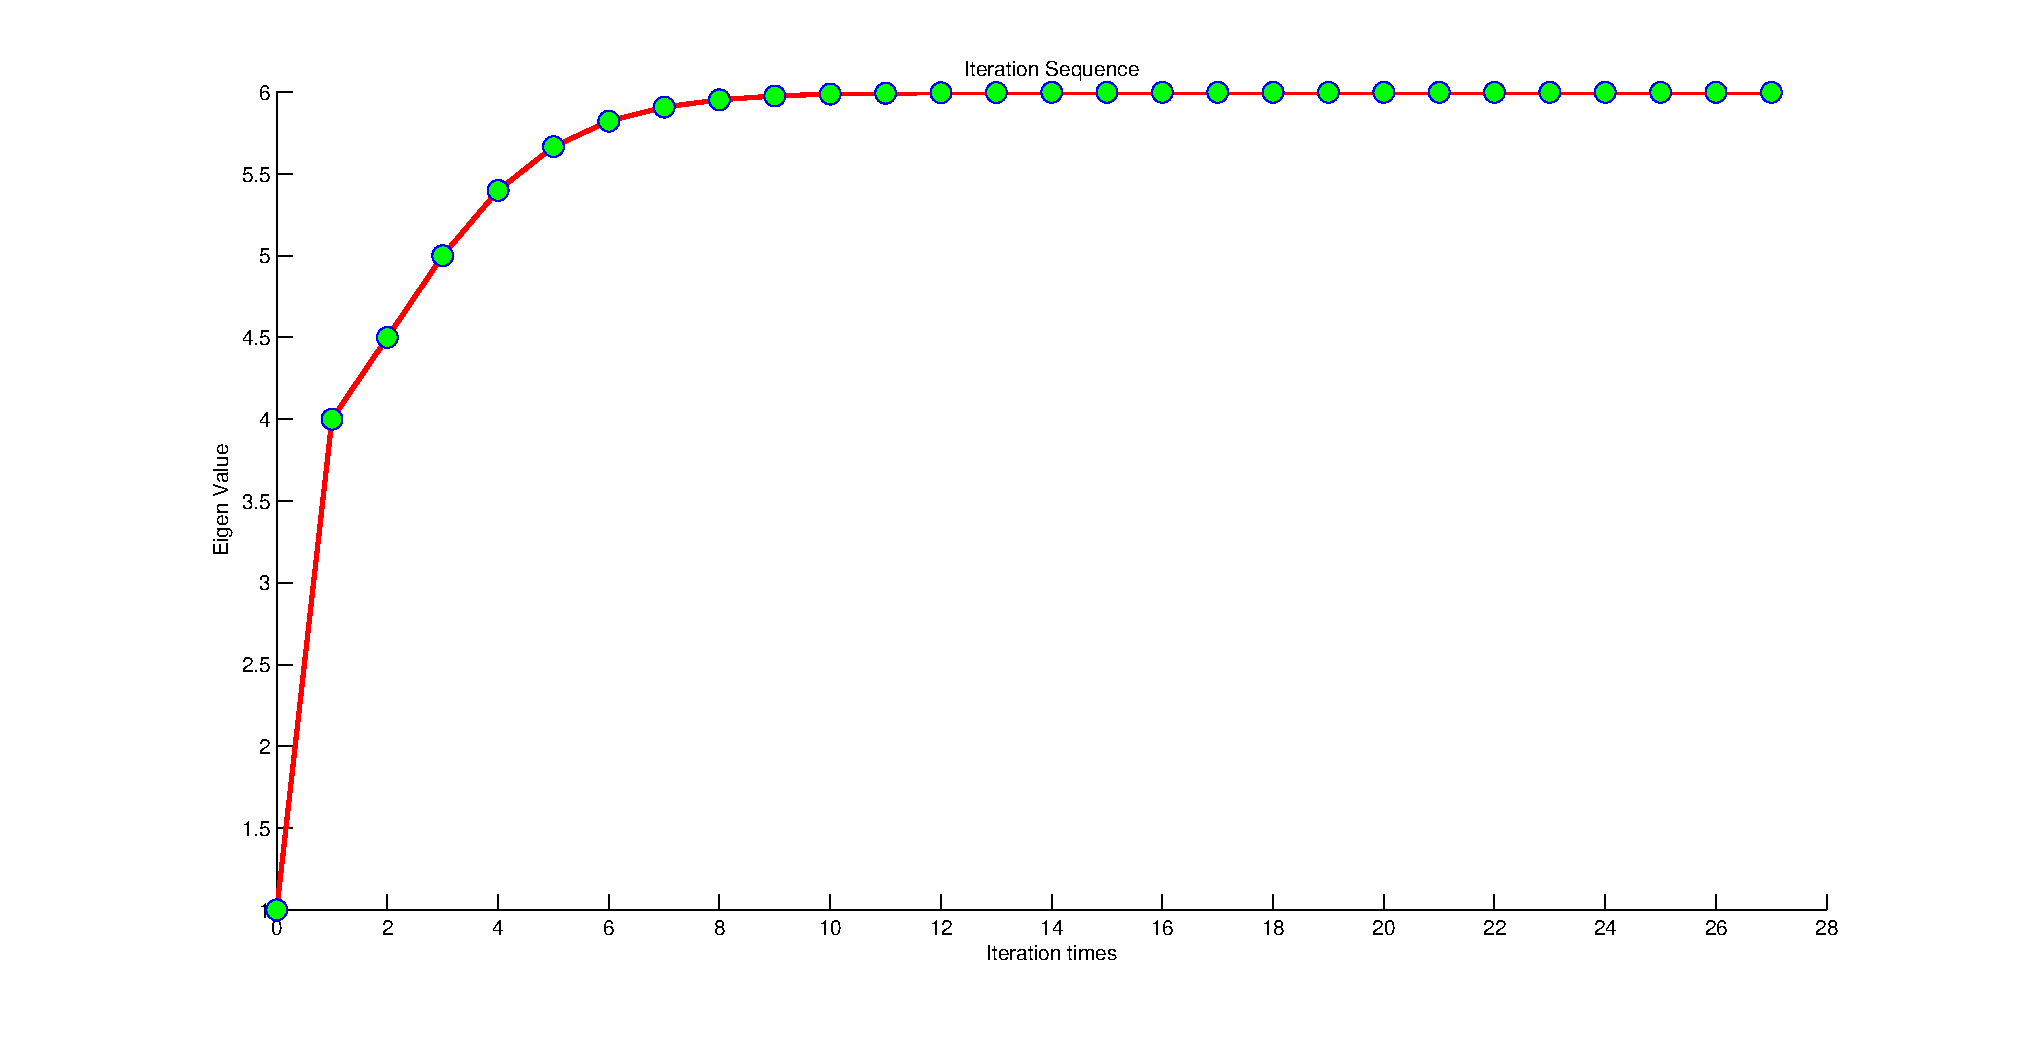
\includegraphics[width=1.0\textwidth]{../chapter_9_1.eps}
						\caption{幂法特征值迭代序列}
						\label{img_chapter9_1}
					\end{figure}
			\paragraph{对称幂法}
				\subparagraph{简介}
					假设$\mathbf{A}$是对称矩阵, $\mathbf{A}$有$n$个实数特征向量$\left|\lambda_1 \right| > \left|\lambda_2 \right| > \cdots > \left|\lambda_n \right|$, 对应$n$个标准正交特征向量$\left\{\mathbf{v}^{\left(1\right)}, \mathbf{v}^{\left(2\right)}, \cdots, \mathbf{v}^{\left(n\right)} \right\}$. 
					
					$\forall \mathbf{x}_0 \in \mathbb{R}^{n}, \mathbf{x}_0 = \beta_1 \mathbf{v}^{\left(1\right)} + \beta_2 \mathbf{v}^{\left(2\right)} + \cdots + \mathbf{v}^{\left(n\right)}$.
					
					对于$\mathbf{x}_k = \mathbf{A}^k \mathbf{x}_0$,$\mathbf{x}_k = \beta_1 \lambda_1^k \mathbf{v}^{\left(1\right)} + \beta_2 \lambda_2^k \mathbf{v}^{\left(2\right)} + \cdots + \beta_n \lambda_n^k \mathbf{v}^{\left(n\right)}$.
					因为$n$个特征向量标准正交, 因此
					$$\mathbf{x}_k^T \mathbf{x}_k = \sum_{j=1}^{n} \beta_j^2 \lambda_j^{2k} = \beta_1^2 \lambda_1^{2k} \left[1 + \sum_{j=2}^{n}\left(\frac{\beta_j}{\beta_1}\right)^2 \left(\frac{\lambda_j}{\lambda_n} \right)^{2k} \right]$$
					且
					$$ \mathbf{x}_k^{T} \mathbf{A} \mathbf{x}_k = \sum_{j=1}^{n} \beta_j^2 \lambda_j^{2k+1} = \beta_1^2 \lambda_1^{2k+1} \left[ 1 + \sum_{j=2}^{n} \left(\frac{\beta_j}{\beta_1}\right)^2 \left(\frac{\lambda_j}{\lambda_1}\right)^{2k+1} \right] $$
					于是
					$$\lim\limits_{k \to \infty} \frac{\mathbf{x}_k^T \mathbf{A} \mathbf{x}_k}{\mathbf{x}_k^T \mathbf{x}_k} = \lambda_1, \lim\limits_{k \to \infty} \frac{\mathbf{x}_k}{\left|\left|\mathbf{x}_k \right|_{2} \right|} = \frac{\mathbf{v}^{\left(1\right)}}{\left|\left|\mathbf{v}^{\left(1\right)} \right| \right|_2}$$.
				\subparagraph{code}
					:\newline
					\begin{lstlisting}
						clear;clc;
						A = [4,-1,1;-1,3,-2;1,-2,3]; n = length(A);
						x = [1;1;1]; N = 1000; TOL = 1e-7;
						x = x/norm(x,2);
						for i = 1:N
							y = A*x; u = x'*y;
							if norm(y,2) < 1e-10
								fprintf('A has eigen value 0. select new vector x and restart.\n')
								return
							end
							norm_y = norm(y,2);
							err = norm(x-y/norm_y,2);
							x = y/norm_y;
							if err < TOL
								fprintf('Answer %f Iteration time %d\n',u,i)
								disp(x')
								return
							end
						end
						fprintf('No Solution\n')
					\end{lstlisting}
				\subparagraph{Answer}
					Max Eigen Value: 6.000000, Iteration time 24 \\
					特征向量: $$\mathbf{x} = \left(0.5774,-0.5774,0.5774\right)$$
					\begin{figure}[H]
						\centering
						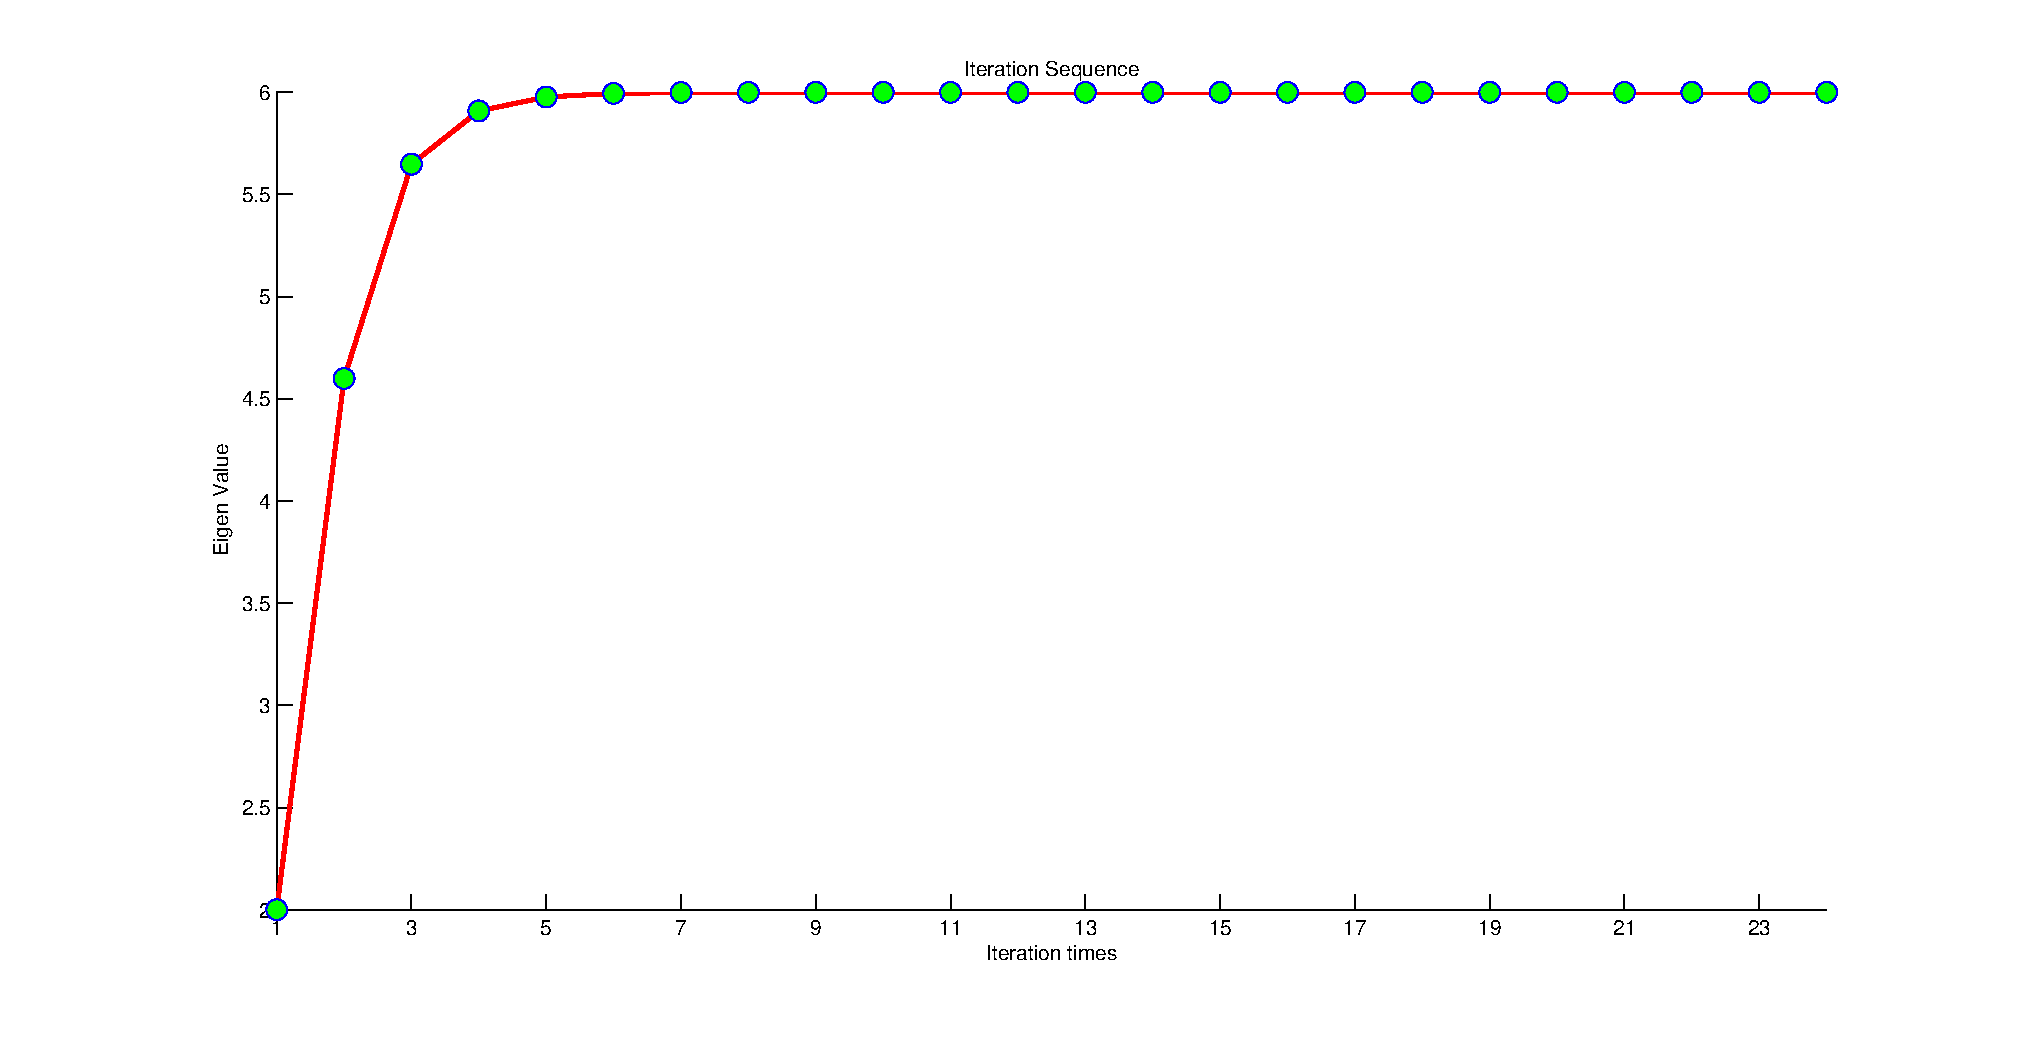
\includegraphics[width=1.0\textwidth]{../chapter_9_2.eps}
						\caption{对称幂法特征值迭代序列}
						\label{img_chapter9_2}
					\end{figure}
			\paragraph{反幂法}
				\subparagraph{推导}
					设$\mathbf{A}$为$n\times n$阶非奇异矩阵, $\lambda$和$\mathbf{v}$为对应的特征向量, 即$\mathbf{Au} = \lambda \mathbf{v}$.
					
					由于$\mathbf{A}^{-1}\mathbf{v} = \frac{1}{\lambda}\mathbf{v}$. 如果$\mathbf{A}$的特征值的顺序为$\left|\lambda_1\ \right| \geq \left|\lambda_2 \right| \geq \cdots \geq \left|\lambda_n \right|$,
					
					则$\mathbf{A}^{-1}$的特征值$\left|\frac{1}{\lambda_n}  \right|\geq \left|\frac{1}{\lambda_{n-1}} \right| \geq \cdots \geq \left|\frac{1}{\lambda_1} \right|$.
					
					因此, 若对矩阵$\mathbf{A}^{-1}$用幂法, 即可计算出$\mathbf{A}^{-1}$的最大特征值$\frac{1}{\lambda_n}$, 从而求得$\mathbf{A}$按模最小的特征值$\lambda_n$.
					
					因为$\mathbf{A}^{-1}$的计算比较麻烦, 因此在实际运算时, 以求解方程组$\mathbf{Ax}^{\left(k+1 \right)} = \mathbf{x}^{\left(k\right)}$替代.
					
					在本题中, 需要求解最大特征值. 根据圆盘定理, 矩阵$\textbf{A}$的特征值有上界$Ma$. 设$\lambda$为$\textbf{A}$的特征值, $k\in \mathbb{R}$. 则$\left(\mathbf{A}-k\mathbf{I}\right)\mathbf{x} = \left(\lambda - k\right) \mathbf{x}$. 此时令$k = Ma + 2$, 则$\left(\mathbf{A} - \left(Ma+2\right)\mathbf{I}\right)$的特征值均小于$0$. 设用反幂法求出$\left(\mathbf{A} - \left(Ma+2\right)\mathbf{I}\right)^{-1}$的绝对值最小特征值为$\left|\lambda^{*}\right|$, 则$\textbf{A}$的最大特征值为$Ma+2-\frac{1}{\left|\lambda^{*} \right|}$.
					
					注: 圆盘定理:设$\mathbf{A}$是一个$n\times n$的矩阵, $\mathbb{R}_i$表示以$a_{ii}$为圆心, $\sum_{j=1,j\neq i}^{n}\left|a_{ij} \right|$的圆. 
					令$$\mathbb{R}_i = \left\{z \in \mathbb{C}\bigg | \left|z-a_{ii} \right| \leq \sum_{j=1,j\neq i}^{n} \left|a_{ij} \right| \right\}$$
					$\mathbf{A}$的特征值包含在$\bigcup_{i=1}^n \mathbb{R}_i $中.
					
					对幂法进行改造, 反幂法计算的主要步骤如下:
					\begin{enumerate}
						\item 对$\mathbf{A}$进行三角形分解$\mathbf{A}=\mathbf{LU}$
						\item 做如下迭代:
						$$\left\{
							\begin{aligned}
								Let\  &\mathbf{x}^{\left(0\right)} = \mathbf{y}^{\left(0\right)} \neq 0 \\
								Solve: &\mathbf{Ax}^{\left(k\right)} = \mathbf{y}^{\left(k-1\right)} \\
								Then: &\mathbf{y}^{\left(k\right)} = \frac{\mathbf{x}^{\left(k\right)}}{\left| \left|\mathbf{x}^{\left(k\right)} \right|\right|_{\infty}}
							\end{aligned}
						\right.$$
					\end{enumerate}
					在反幂法中, 最终得到的$\mathbf{x}$即为所求特征向量.
				\subparagraph{Code}
					:\newline
					\begin{lstlisting}
					clear;clc;
					A = [4,-1,1;-1,3,-2;1,-2,3]; n = length(A); TOL = 1e-7;
					Ma = zeros(1,n);
					for i=1:n
						for j=1:n
							if i==j
								Ma(i) = Ma(i) + A(i,i);
							else
								Ma(i) = Ma(i) + abs(A(i,j));
							end
						end
					end
					change = max(Ma) + 2; A = A - change*eye(n);
					L=eye(n,n); U=zeros(n,n);
					for k=1:n
						for j=k:n
							U(k,j)=A(k,j)-sum(L(k,1:k-1).*U(1:k-1,j)');
						end
						for i=k+1:n
							L(i,k)=(A(i,k)-sum(L(i,1:k-1).*U(1:k-1,k)'))/U(k,k);
						end
					end
					x0 = [1;1;1]; MAXN = 100; mx0 = max(x0);y0 = x0/mx0;
					for CNT = 1:MAXN
						b = y0;
						X=zeros(1,3);Y=zeros(1,3);
						Y(1)=b(1);
						for i=2:n    
							for j=1:i-1
								b(i)=b(i)-L(i,j)*Y(j);
							end
							Y(i)=b(i);
						end
						X(n)=Y(n)/U(n,n);
						for i=(n-1):-1:1
							for j=n:-1:i+1
								Y(i)=Y(i)-U(i,j)*X(j);
							end
							X(i)=Y(i)/U(i,i);
						end
						x = X';mx = max(x); y0 = x/mx;
						if abs(mx-mx0) < TOL
							fprintf('Answer %f Iteration time %d\n',change-1/mx,CNT)
							disp(x)
							return
						end
						x0 = x; mx0 = mx;
					end
					fprintf('No solution')
					\end{lstlisting}
				\subparagraph{Answer}
					 Max Eigen Value: 6.000000, Iteration time 20 \\
					 Eigen Vector: $\mathbf{x} = \left(-0.5000,0.5000 ,-0.5000\right)^T$
					\begin{figure}[H]
					 	\centering
					 	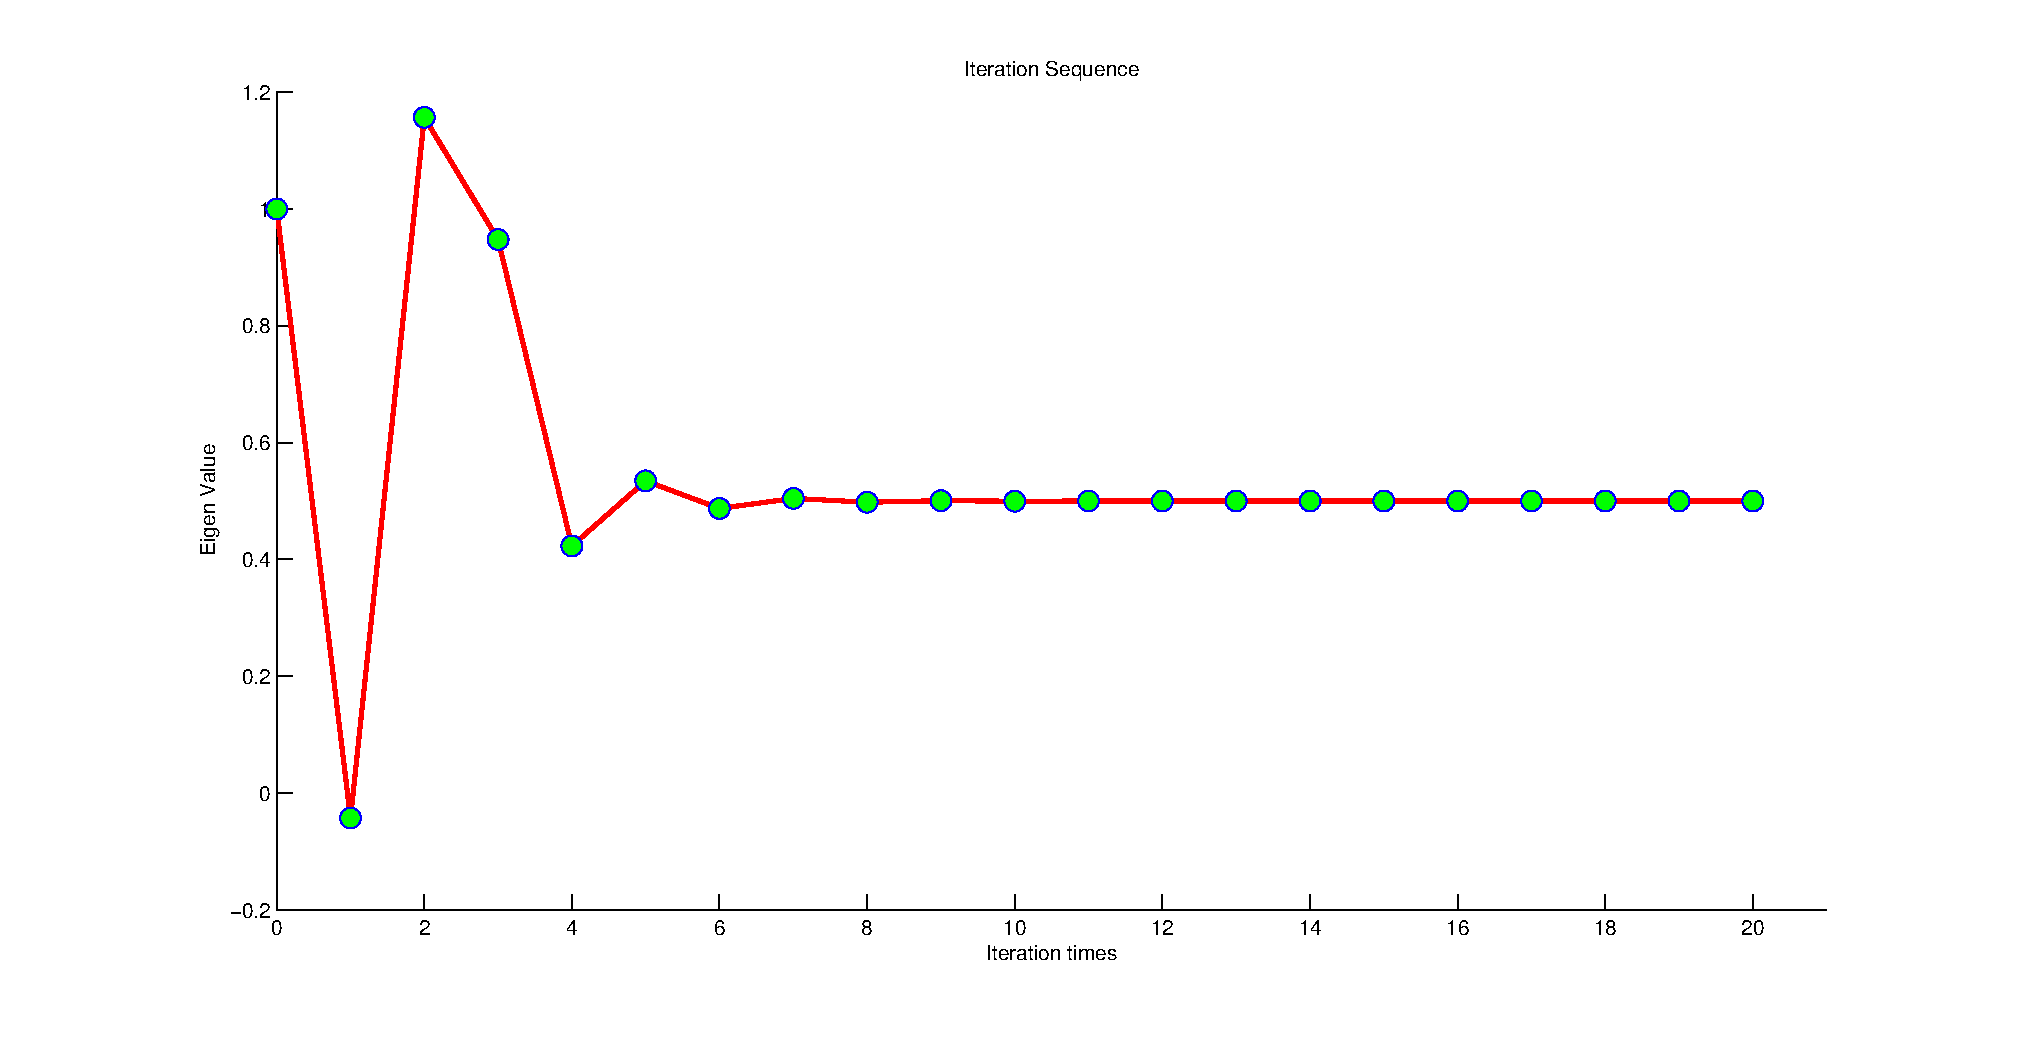
\includegraphics[width=1.0\textwidth]{../chapter_9_3.eps}
					 	\caption{反幂法特征值迭代序列}
					 	\label{img_chapter9_3}
					 \end{figure}
	\section{Conclusion}
		在本学期数值计算实验中, 我掌握了如下技能:
		\begin{enumerate}
			\item MATLAB的基本使用方式;
			\item 二分法、牛顿法;
			\item 多项式插值, 包括拉格朗日插值、Hermite插值等;
			\item 根据插值多项式进行数值积分;
			\item 求给定初始条件的常微分方程组;
			\item 求解矩阵特征值;
			\item 求解线性方程组;
			\item 通过最小二乘进行多项式拟合;
			\item 加深对数学分析、高等代数的理解;
			\item Latex的使用;
			\item 误差分析.
		\end{enumerate}
		最后, 感谢刘保东老师, 在本学期的数值计算课程中, 让我对数学、计算有了新的认识.
\end{CJK*}
\end{document}